\chapter{Performance Evaluation}
\label{cha:evaluation}
\vspace{0.4 cm}

In this chapter, the proposed system is validated and the performance of the models for the different use cases is evaluated.
The first section presents the datasets provided by MIWEnergia\footnote{ \url{https://www.miwenergia.com/} }.
Subsequently, the adapted evaluation methodology is described.
Finally, the evaluation of the performance of the models for the different use cases is presented.
After this chapter, it will be clear how the system has been validated and what the performance achieved by the proposed system is.


\section{MIWEnergia datasets}
\label{sec:datasets}
\vspace{0.2 cm}

In this section, the MIWEnergia datasets are described.
They provided 3 kinds of datasets: aggregated consumption data from all their customers, consumption data from single customers, and production data from PV plants.

\begin{figure}[H]
\begin{minipage}[b]{8.5cm}
\centering
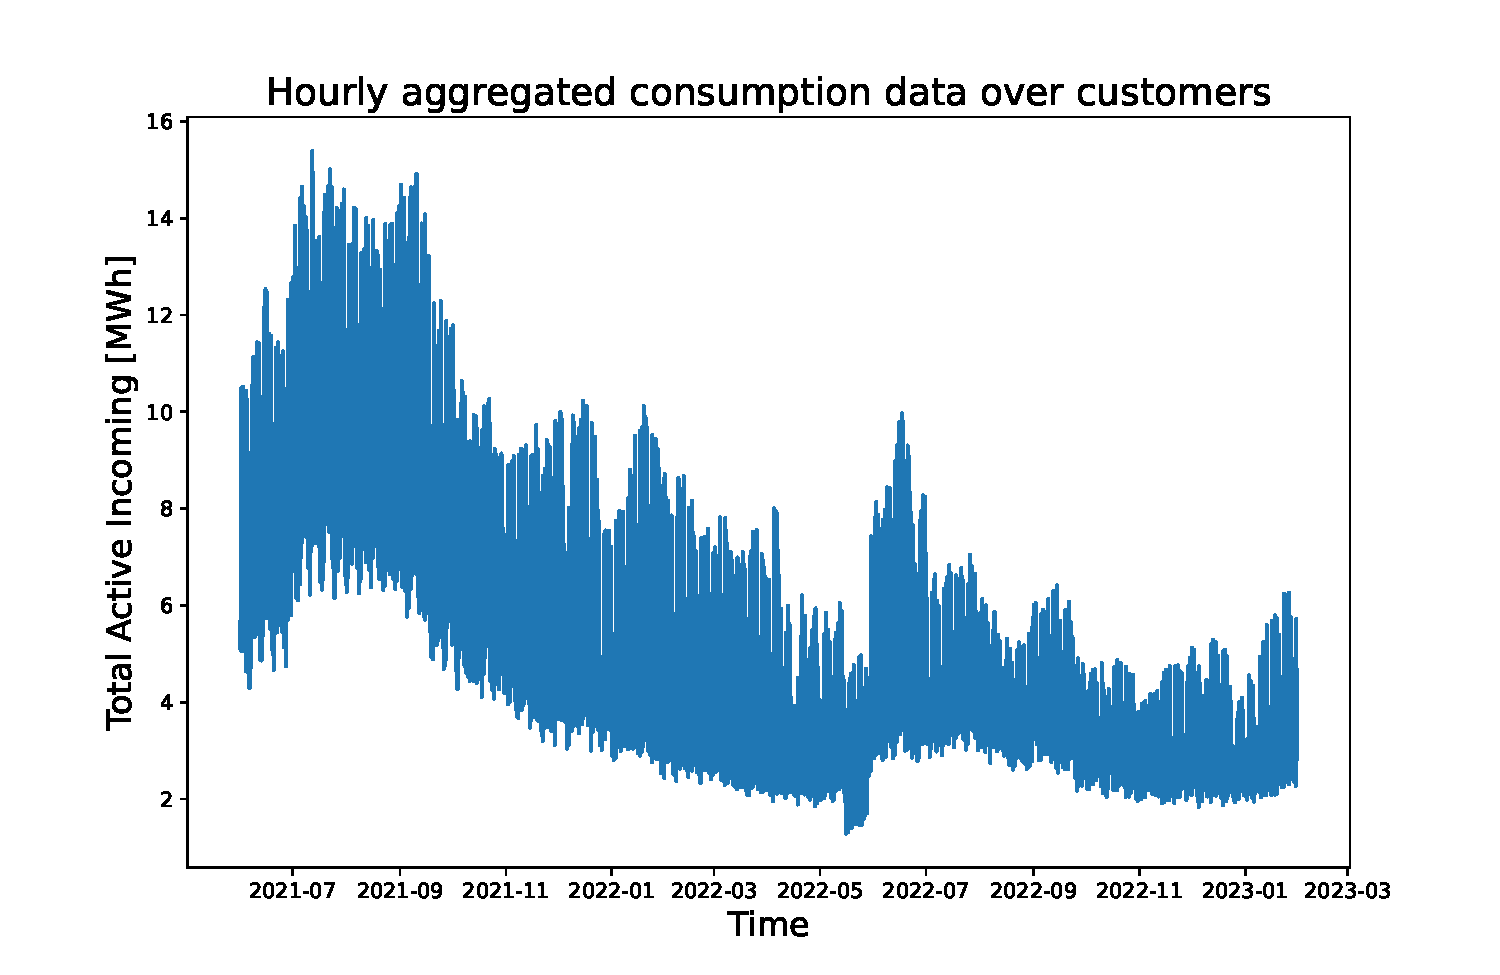
\includegraphics[width=1\textwidth]{images/demand/data_plot}
\subcaption{}
\label{fig:demanddataplot}
\end{minipage}
\ \hspace{2mm} \
\begin{minipage}[b]{8.5cm}
\centering
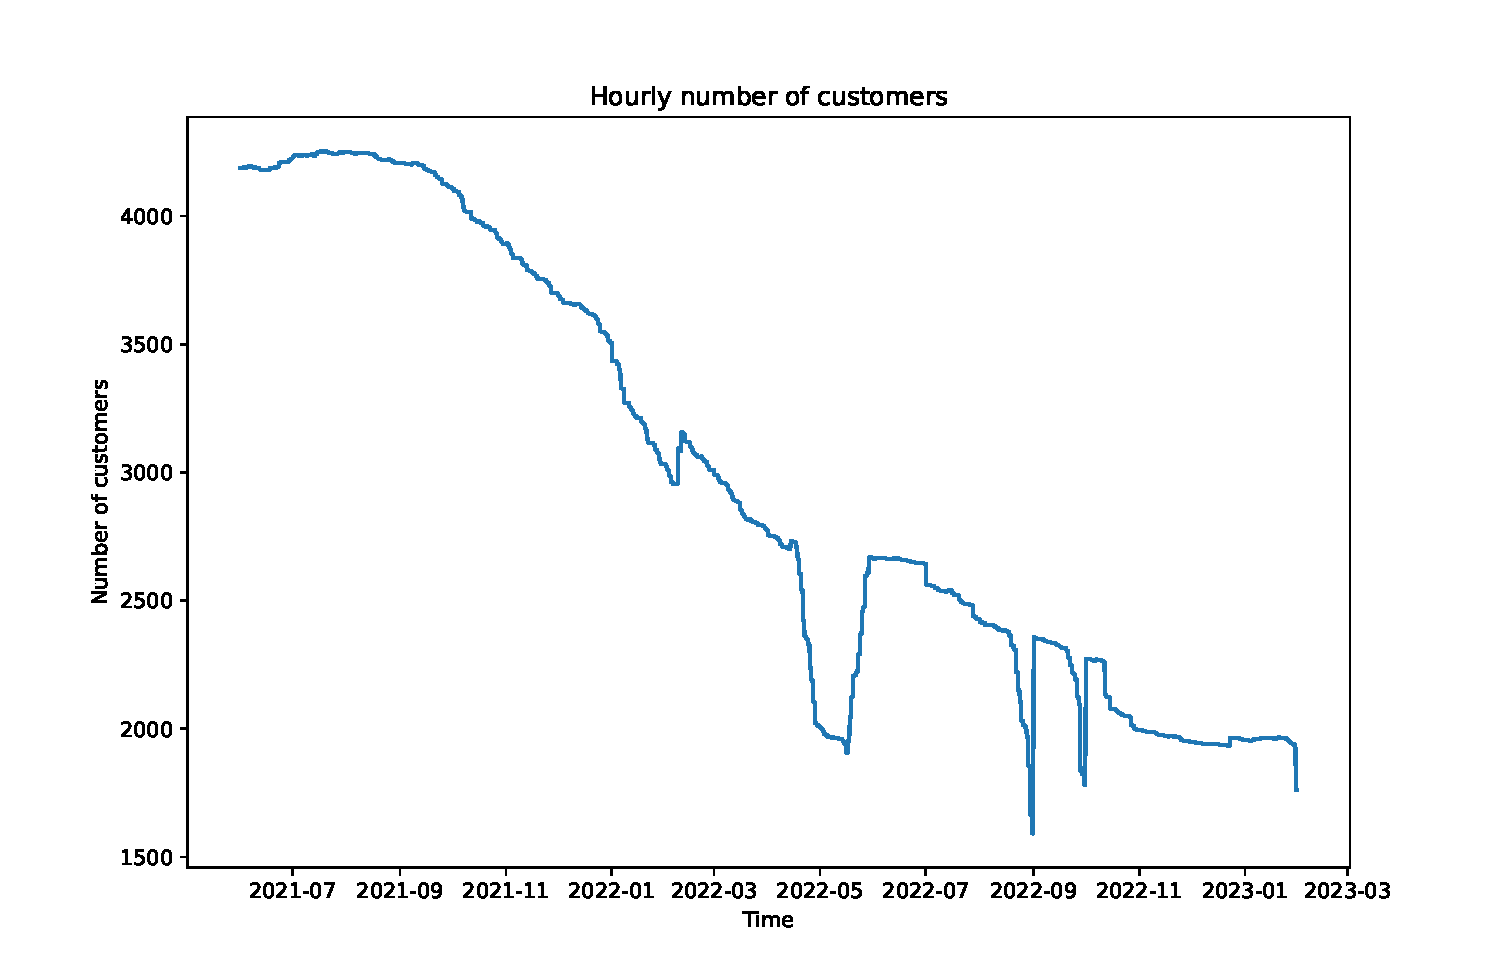
\includegraphics[width=1\textwidth]{images/demand/customers_plot}
\subcaption{}
\label{fig:customersplot}
\end{minipage}
\begin{minipage}[b]{17cm}
\centering
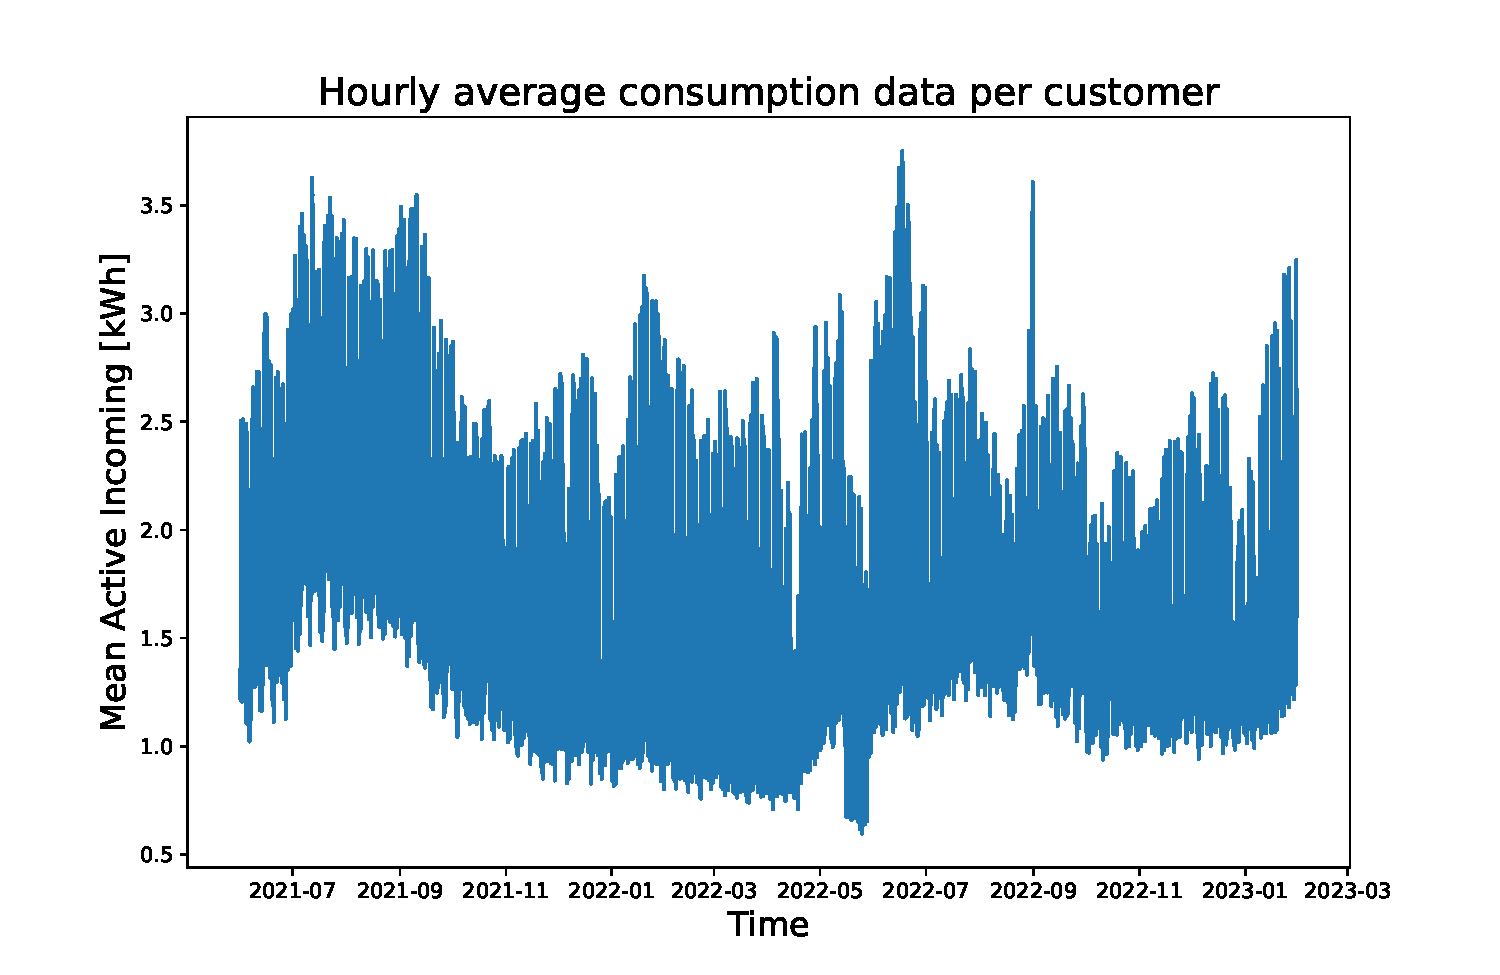
\includegraphics[width=0.5\textwidth]{images/demand/mean_data_plot}
\subcaption{}
\label{fig:meandemanddataplot}
\end{minipage}
\caption{The graphical representation of the hourly \subref{fig:demanddataplot} aggregated consumption over customers, \subref{fig:customersplot} number of customers, and \subref{fig:meandemanddataplot} average consumption per customer.}
\end{figure}

The aggregated consumption data from all their customers consists of hourly aggregated consumption data from June 2021 to January 2023 for a total of 14617 entries.
The graphical representation of the hourly aggregated consumption data is reported in figure~\ref{fig:demanddataplot}.
The number of customers is variable, with a maximum of 4253, a minimum of 1591, a mean of 2988, and a standard deviation of 855.
The graphical representation of the hourly number of customers is reported in figure~\ref{fig:customersplot}.
It was thought to normalize the consumption on the basis of the number of customers in order to study the average consumption per user, as illustrated in figure~\ref{fig:meandemanddataplot}, and then multiply by the number of customers.
However, this was not feasible since often this value changes significantly without reflecting on the consumption data, this information was deemed unreliable and not utilized.
Despite this limitation, the average consumption per customer still provided valuable insights into consumption patterns.
Specifically, it suggested the presence of two consumption peaks: one in the summer, likely attributed to air conditioning systems, and a second peak in the winter, likely caused by heating systems.

The consumption data from single customers consists of hourly aggregated consumption data of three customers:
\begin{enumerate}
  \item from June 2021 to August 2022 for a total of 10952 total entries and it is represented in figure~\ref{fig:dataplotcustomer1};
  \item from September 2021 to May 2022 for a total of 5855 total entries and it is represented in figure~\ref{fig:dataplotcustomer2};
  \item from September 2021 to August 2022 for a total of 8760 total entries and it is represented in figure~\ref{fig:dataplotcustomer3}.
\end{enumerate}
The total entries for the three customers are 25567 in the overall period from June 2021 to August 2022.

\begin{figure}[H]
\begin{minipage}[b]{8.5cm}
\centering
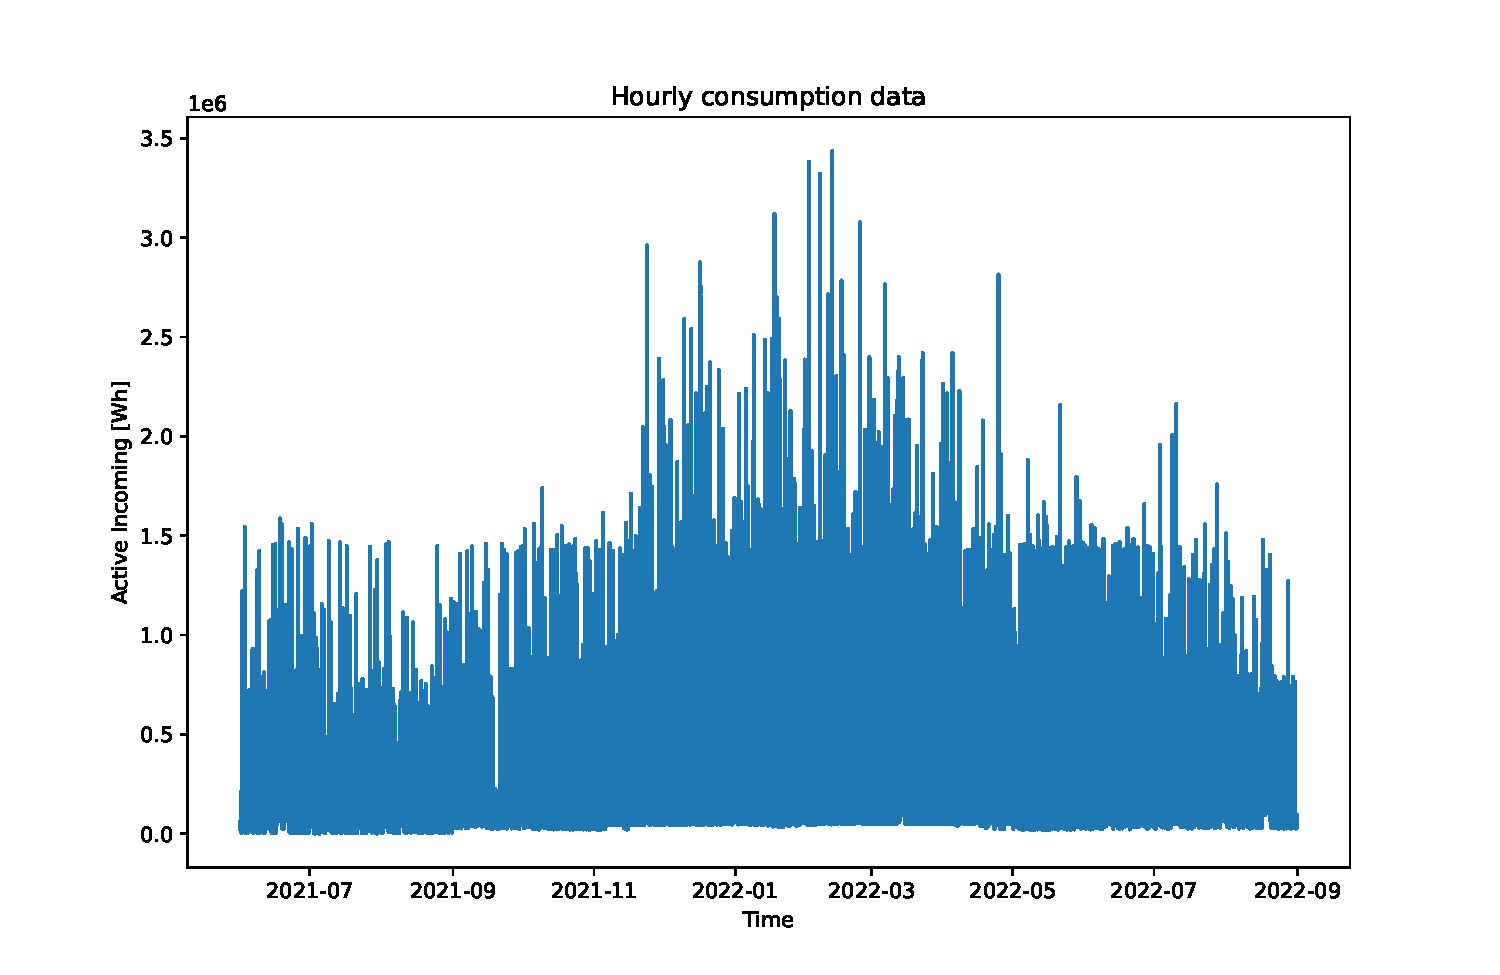
\includegraphics[width=1\textwidth]{images/baseline/data_plot_customer1}
\subcaption{First customer.}
\label{fig:dataplotcustomer1}
\end{minipage}
\ \hspace{2mm} \
\begin{minipage}[b]{8.5cm}
\centering
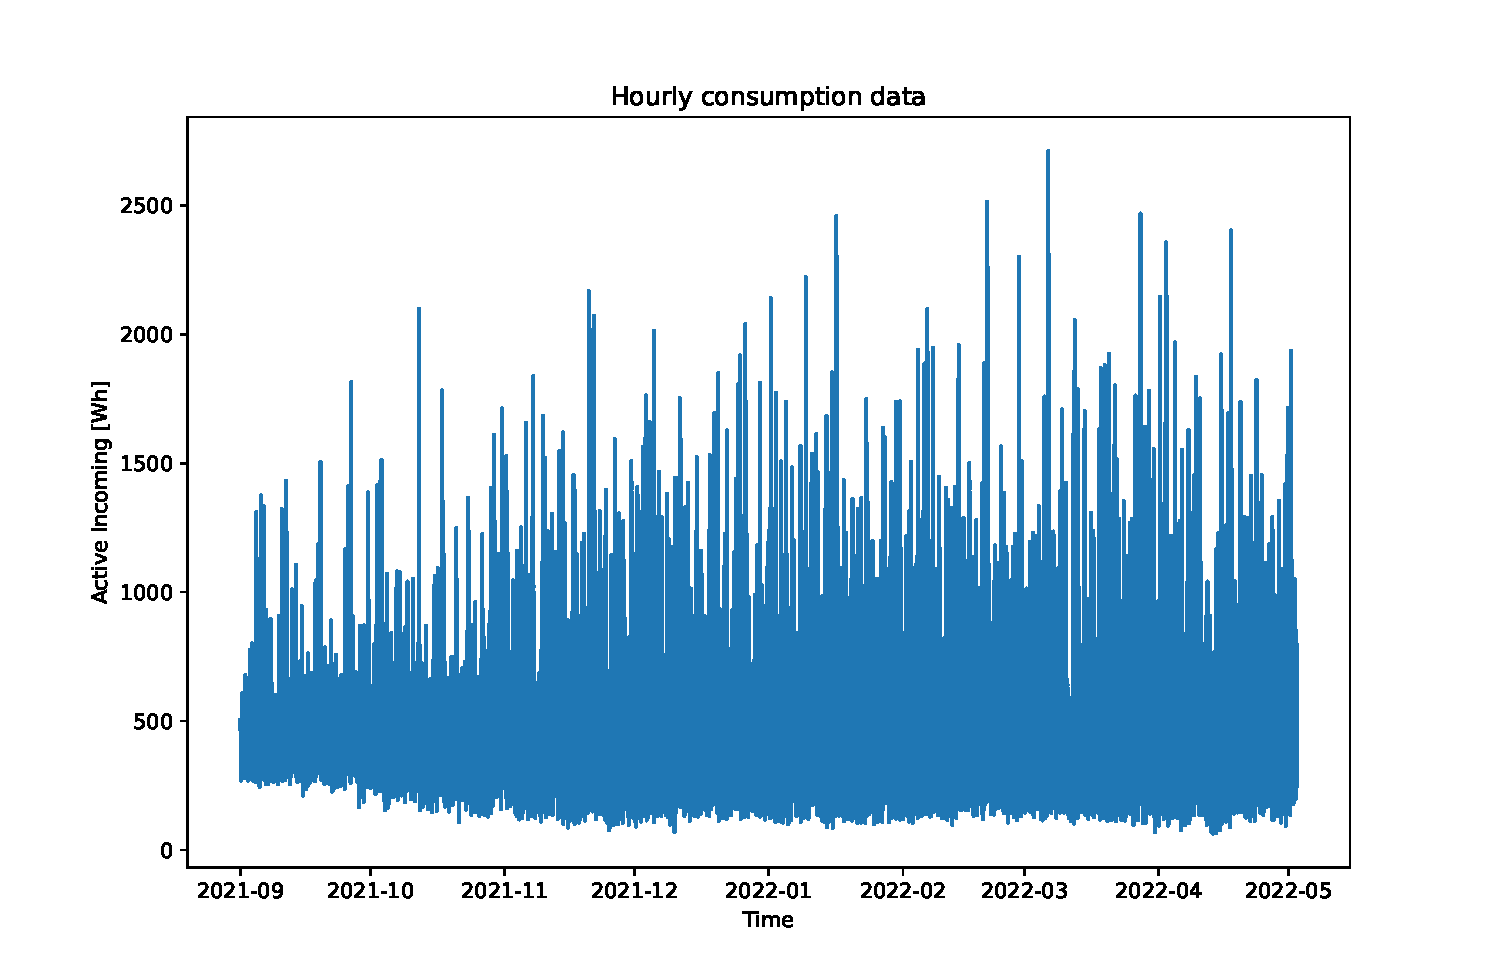
\includegraphics[width=1\textwidth]{images/baseline/data_plot_customer2}
\subcaption{Second customer.}
\label{fig:dataplotcustomer2}
\end{minipage}
\begin{minipage}[b]{17cm}
\centering
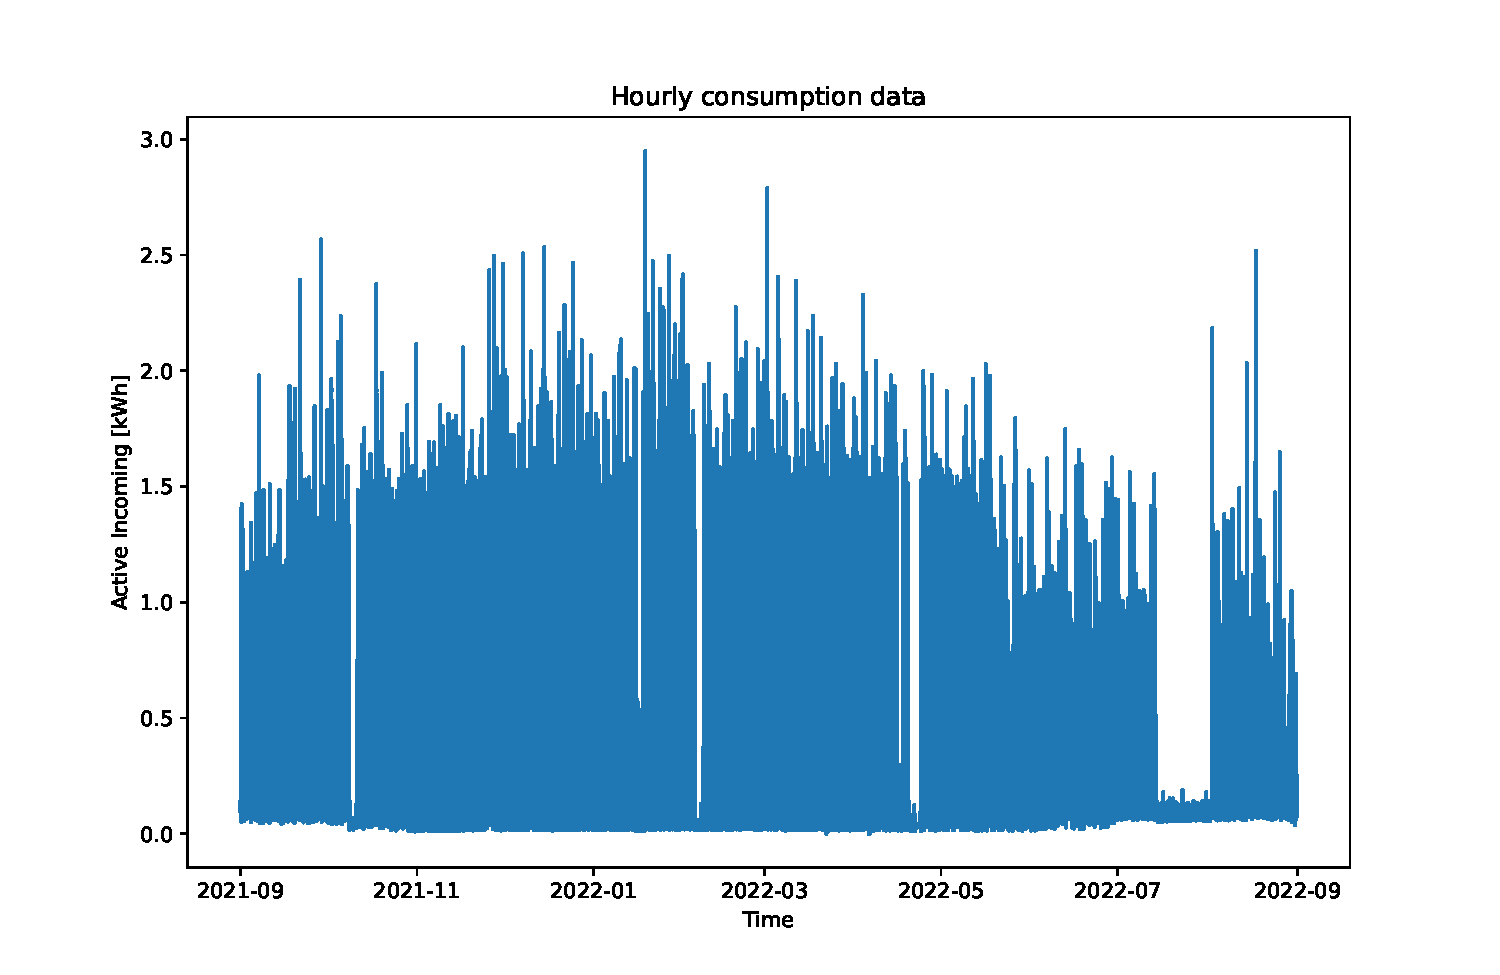
\includegraphics[width=0.5\textwidth]{images/baseline/data_plot_customer3}
\subcaption{Third customer.}
\label{fig:dataplotcustomer3}
\end{minipage}
\caption{The graphical representation of the consumption data of the three customers.}
\end{figure}

Only consumption data for three customers were provided, as electricity consumption data of customers is considered personal data as stated in the Directive (EU) 2019/944 of the European Parliament\footnote{ \url{https://eur-lex.europa.eu/legal-content/EN/TXT/?uri=CELEX:32019L0944} }, which establishes common rules for the internal market for electricity.
As such, the data falls under the scope of the General Data Protection Regulation (GDPR)\footnote{ \url{https://gdpr-info.eu/} }, which requires explicit consent for processing personal data.
Therefore, it is likely that the provided data came from MIWEnergia's internal employees who consented to participate in the research.
In fact, the provided data were needed for a technical feasibility study.
However, to identify consumption patterns among a broader population, data from more customers would be required.

By analyzing the data plots, it can be observed that the consumption patterns of the three customers are quite distinct.
For instance:
\begin{itemize}
  \item The first customer's consumption is consistently below 1.5 kWh throughout the year except for the winter season;
  \item The second customer shows almost the same consumption pattern;
  \item The third customer has a dense series with some gaps with very low consumption in parts of the year, probably due to time periods away from home.
\end{itemize}

The production data from 8 PV plants consists of hourly aggregated production data:
\begin{enumerate}
  \item from January 2022 to October 2022 for a total of 7296 total entries and it has a nominal power of 149.75 kW;
  \item from February 2022 to October 2022 for a total of 6552 total entries and it has a nominal power of 237.6 kW;
  \item from February 2022 to October 2022 for a total of 6552 total entries and it has a nominal power of 158.4 kW;
  \item from June 2022 to October 2022 for a total of 3576 total entries and it has a nominal power of 1240 kW;
  \item from September 2022 to October 2022 for a total of 1465 total entries and it has a nominal power of 126.2 kW;
  \item from September 2022 to October 2022 for a total of 1465 total entries and it has a nominal power of 113 kW;
  \item from September 2022 to October 2022 for a total of 1465 total entries and it has a nominal power of 45 kW;
  \item from September 2022 to October 2022 for a total of 1465 total entries and it has a nominal power of 100 kW;
\end{enumerate}
The total entries for the 8 PV plants are 29836 total entries in the overall period from January 2022 to October 2022, aggregating over plants the resulting entries are 7296.
The graphical representation of the hourly aggregated total and mean percentage production data are reported respectively in figure~\ref{fig:productiondataplot} and figure~\ref{fig:productiondataplotpercentage}.

The same weather data from the same provider and the same weather station were used for all the tasks.
While it is reasonable to assume that some weather conditions, such as clouds, may vary and affect consumption and production differently, this approach was taken since the customers and the PV plants were in the same area, with a maximum distance of around 100 km between them, and also because the value of the weather parameters is an average of the values recorded in the past hour.
Therefore, using the same weather data is deemed appropriate for the analysis at hand, given that it reflects the weather conditions in the area over a broad time frame.

\begin{figure}[H]
\begin{minipage}[b]{8.5cm}
\centering
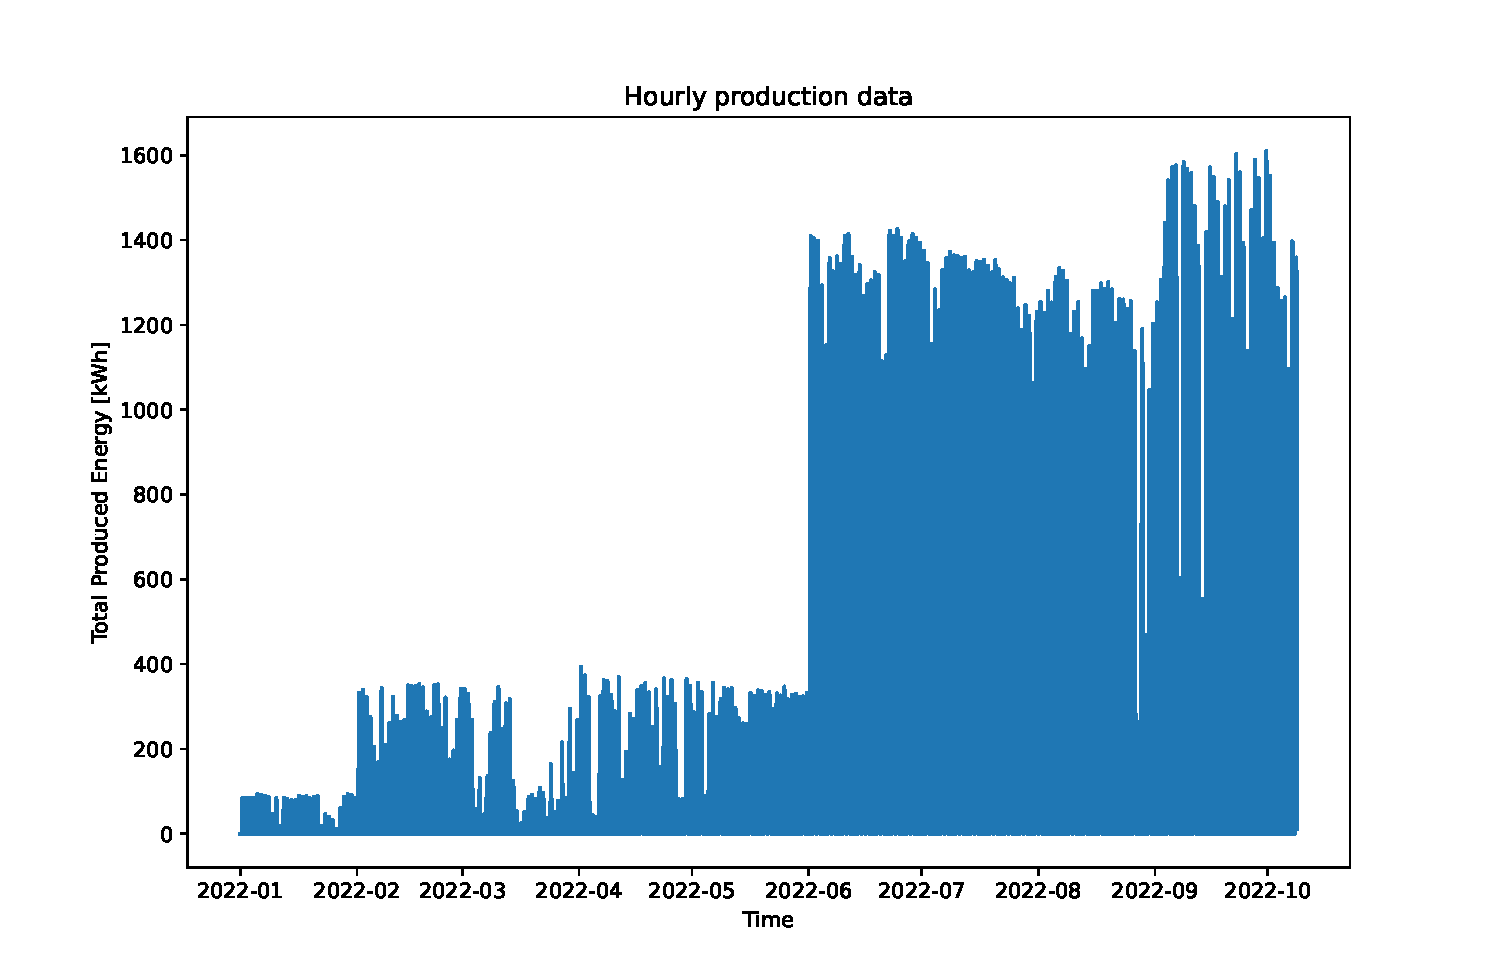
\includegraphics[width=1\textwidth]{images/production/data_plot}
\subcaption{}
\label{fig:productiondataplot}
\end{minipage}
\ \hspace{2mm} \
\begin{minipage}[b]{8.5cm}
\centering
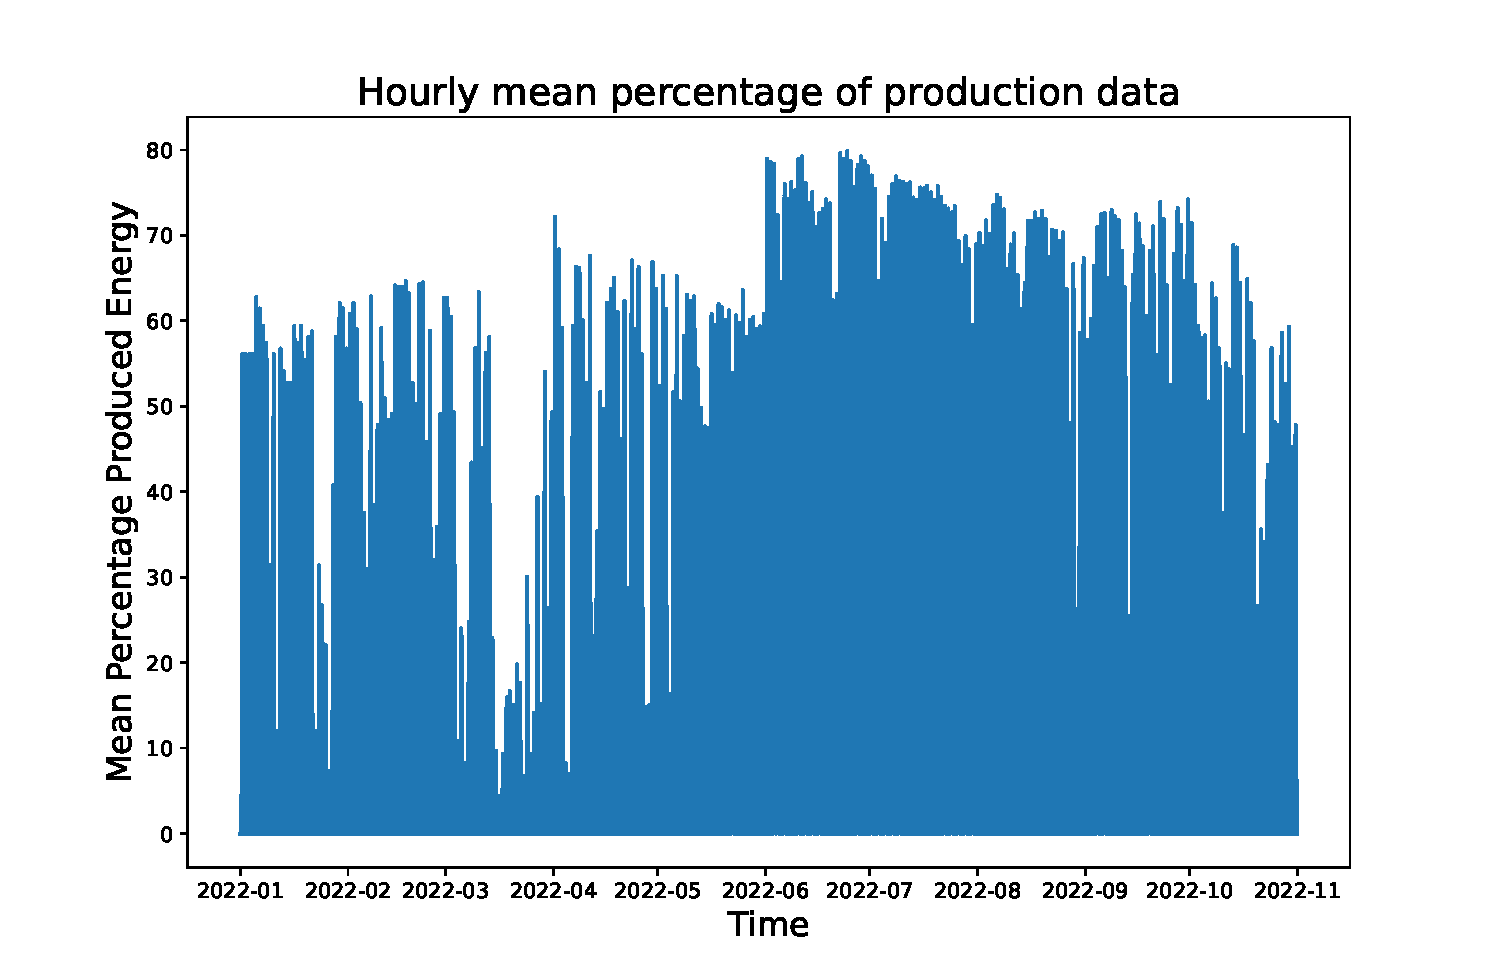
\includegraphics[width=1\textwidth]{images/production/data_plot_percentage}
\subcaption{}
\label{fig:productiondataplotpercentage}
\end{minipage}
\caption{The graphical representation of the hourly aggregated \subref{fig:productiondataplot} total and \subref{fig:productiondataplotpercentage} mean percentage production data.}
\end{figure}


\section{Evaluation methodology}
\label{sec:methodology}
\vspace{0.2 cm}

The evaluation methodology was based on two relevant error metrics: Mean Absolute Percentage Error (MAPE) and Mean Absolute Error (MAE).
These are standard and widely used metrics in time series forecasting for different use cases, as reported in many articles and books such as \cite{armstrong2001principles, DEGOOIJER2006443, HYNDMAN2006679}.
The MAPE is defined as $\text{MAPE}(y, \hat{y}) = \frac{100\%}{N} \sum_{i=0}^{N - 1} \frac{|y_i - \hat{y}_i|}{|y_i|}$.
It is the most relevant error metric for all the tasks since it is a percentage-based error metric that takes into account the magnitude of the errors relative to the actual values.
The MAE is defined as $\text{MAE}(y, \hat{y}) = \frac{ \sum_{i=0}^{N - 1} |y_i - \hat{y}_i| }{N}$.
It is the most suitable error metric in consumption baseline forecasting where there is a high variability from very low to high values, and electricity production forecasting where there is a significant number of zeros when the sun is absent.

\begin{figure}[H]
\centering
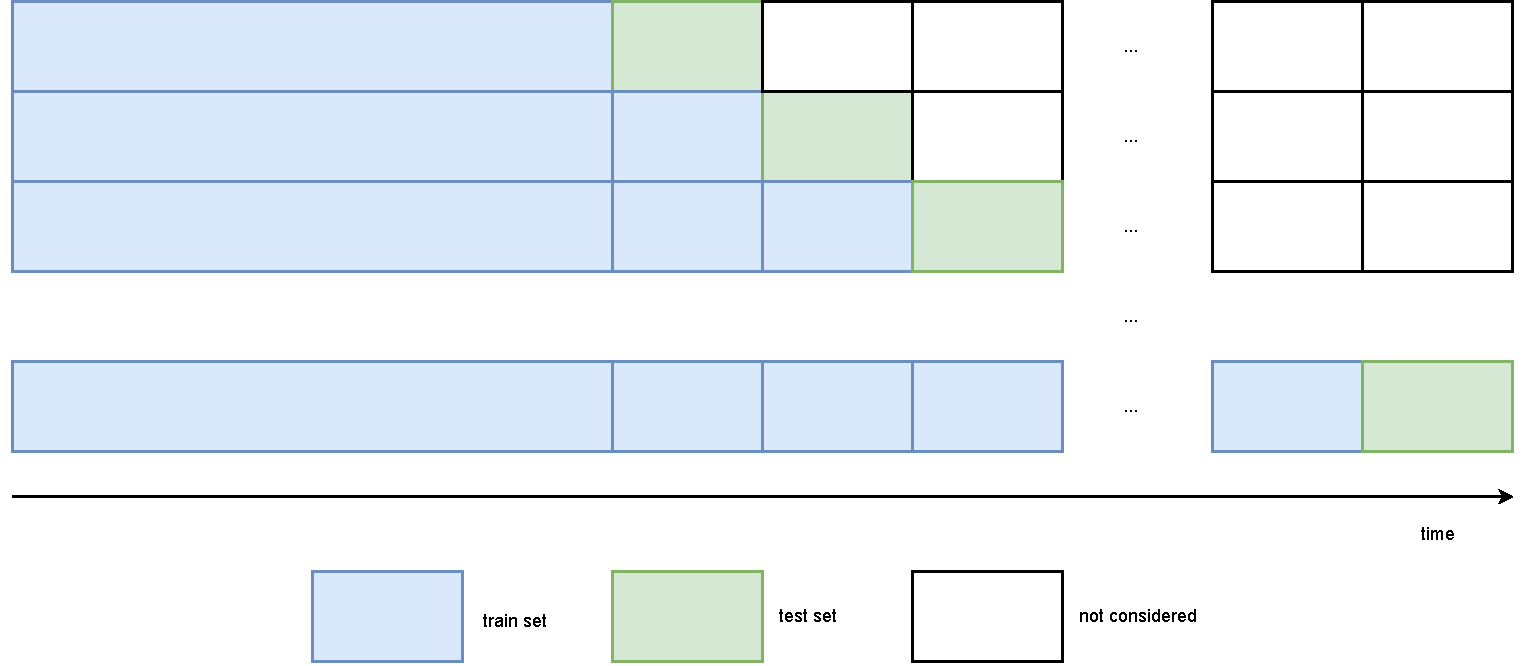
\includegraphics[width=0.8\textwidth]{images/cross_validation}
\caption{The schematic representation of the blocked k-fold cross-validation adopted.}
\label{fig:crossvalidation}
\end{figure}

For assessing the model performance when dealing with time series data, the traditional cross-validation techniques are not suitable as they assume that the data points are independent and identically distributed (i.i.d.), which is not the case in time series data, as also reported in the chapter~\ref{cha:soa} by the following articles \cite{BERGMEIR2012192, Cerqueira2020}.
In fact, in time series data the order of the observations matters, and there are temporal dependencies between the observations.
Therefore, a more appropriate technique for evaluating time series models is blocked k-fold cross-validation.
The basic idea of blocked k-fold cross-validation is to split the data considering multiple training and test sets, where the training set only includes data from the past and the test set includes data from the future.
This simulates the real-world scenario where we want to make predictions about the future based on past data.
In figure~\ref{fig:crossvalidation}, the schematic representation of how the blocked k-fold cross-validation was performed is reported, 12 splits were used with a test size depending on the specific use case.
The training set is increased by adding the previous test elements at every successive evaluation.

Another technique, reported in \cite{Cerqueira2020} is the repeated Holdout Out‐of‐sample tested in multiple testing periods with a Monte Carlo simulation using 70\% of the total observations of the time series in each test.
For each period, a random point is picked from the time series.
The previous window comprising 60\% of the time series is used for training and the following window of 10\% of the time series is used for testing.
In the paper, it was stated that the approach provided the most accurate estimates when the time series are non-stationary.
However, for having the same evaluation mechanisms on all the models and simulating the fact that the model starts with limited data and then the training amount increases over time to obtain better performance, block validation was used using the TimeSeriesSplit provided by the scikit-learn library.
Moreover, the considered data are without a strong trend as reported in the dedicated sections of the specific use cases where the data and the model forecasts are analyzed.

In addition to the blocked k-fold cross-validation results also the results on the last test split using the rest as training are reported.
This was done since it provides insight on which could be the performance of the models in forecasting the near future data with the currently available training data.
A table summarizing the metrics and the evaluation mechanisms adopted is reported in table~\ref{tab:metricstable}.

\begin{table}[H]
\centering
\begin{tabular}{|c|c|}
\hline
\textbf{Metrics} & \textbf{Evaluation mechanisms}\\
\hline
MAPE, MAE & blocked k-fold cross-validation, last test split\\
\hline
\end{tabular}
\caption{Table summarizing the metrics and the evaluation mechanisms adopted.}
\label{tab:metricstable}
\end{table}


\section{Electricity demand forecasting}
\label{sec:demandval}
\vspace{0.2 cm}

The aggregated consumption data over the customers is analyzed to get some descriptive analytics before finding adequate models to forecast the demand.
The time series decomposition using an additive model of the hourly aggregated consumption over the customers considering as period of the time series a week is reported in figure~\ref{fig:demanddecomposition}.
It showed a considerable amount of noise, comparable to seasonality in magnitude.
The trend showed 2 peaks during the summer season, the first being more emphasized since corresponds also to a peak in the number of users.

\begin{figure}[H]
\centering
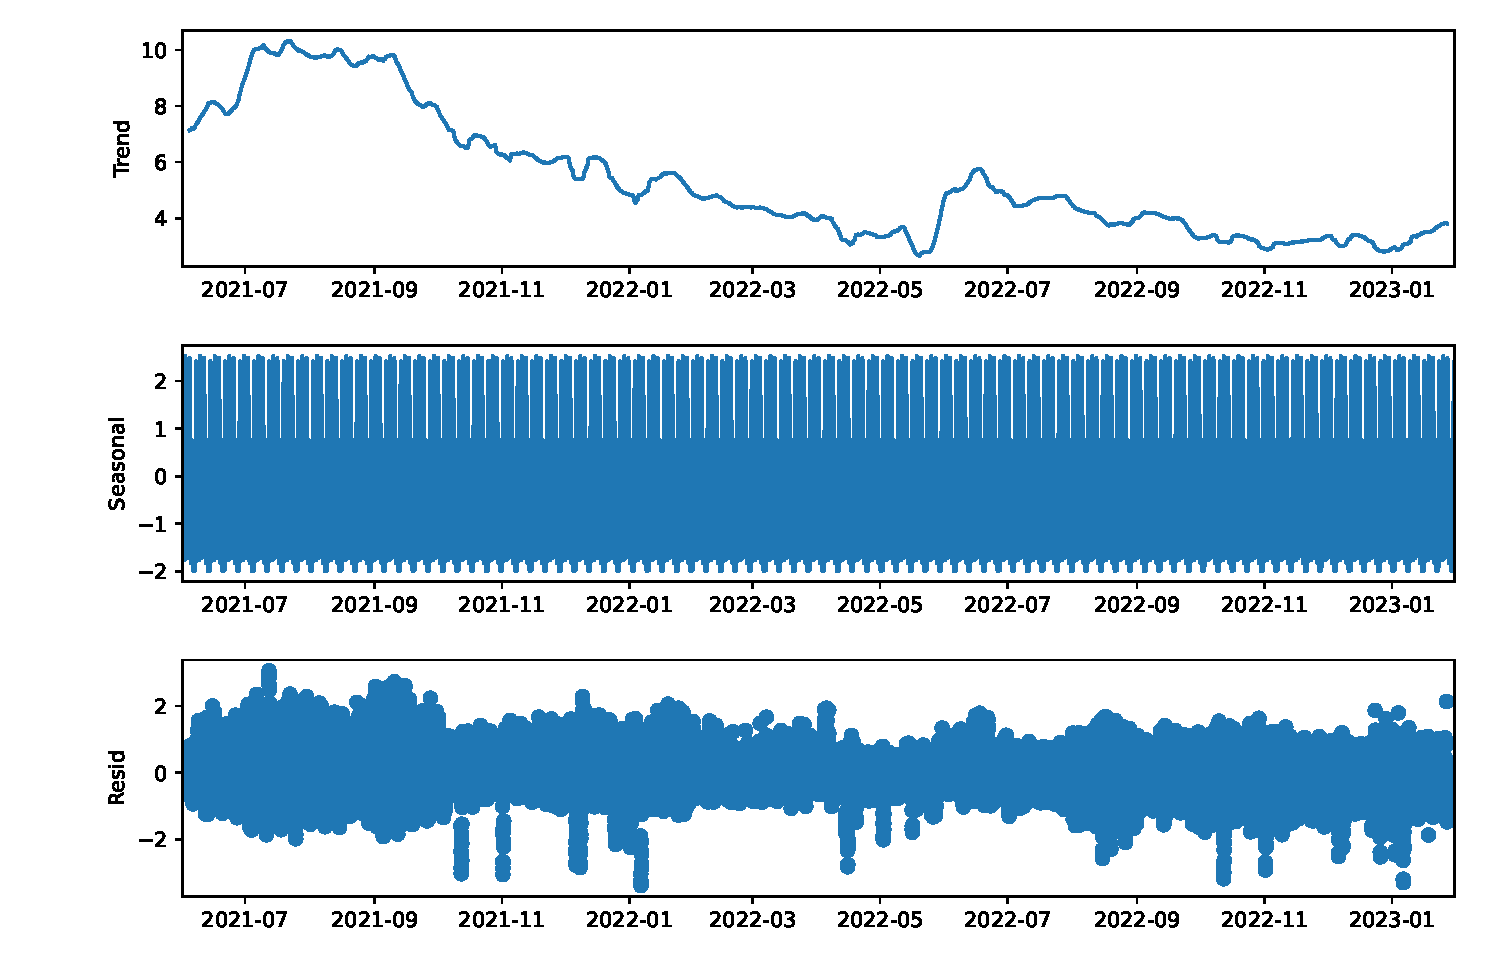
\includegraphics[width=0.5\textwidth]{images/demand/hourly_decomposition_week_period}
\caption{The time series decomposition of the hourly aggregated consumption over the customers considering as period of the time series a week.}
\label{fig:demanddecomposition}
\end{figure}

The auto-correlation of the hourly aggregated consumption over the customers is reported in figure~\ref{fig:demandcorrelation}.
It shows a high auto-correlation value in the close time lags and also at every 24 hours, along with an even higher value at a one-week distance.
This indicates that the consumption data from the closest time lags, particularly up to three closest ones, as well as those corresponding to the same hour in the preceding days and even better in the preceding weeks, may be valuable features for predicting a time instant's demand.
A reasonable balance can be achieved by incorporating the consumption data from the past 14 days.

\begin{figure}[H]
\centering
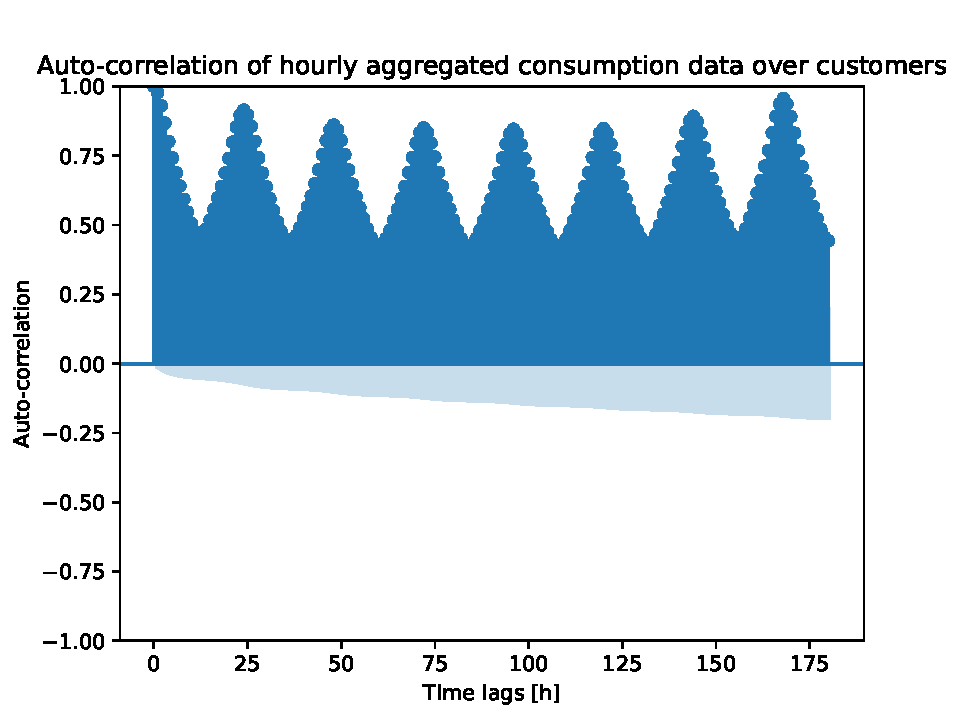
\includegraphics[width=0.4\textwidth]{images/demand/hourly_correlation_week_range}
\caption{The auto-correlation of the hourly aggregated consumption over the customers.}
\label{fig:demandcorrelation}
\end{figure}

The coefficients given by the Fourier transform for the hourly aggregated consumption over the customers are reported in figure~\ref{fig:demandft}.
The graphical representation shows 2 main frequencies, one representing the weekly periodicity and one the daily periodicity.
Other minor peaks are present mostly at multiples of the 1/week frequency.

\begin{figure}[H]
\centering
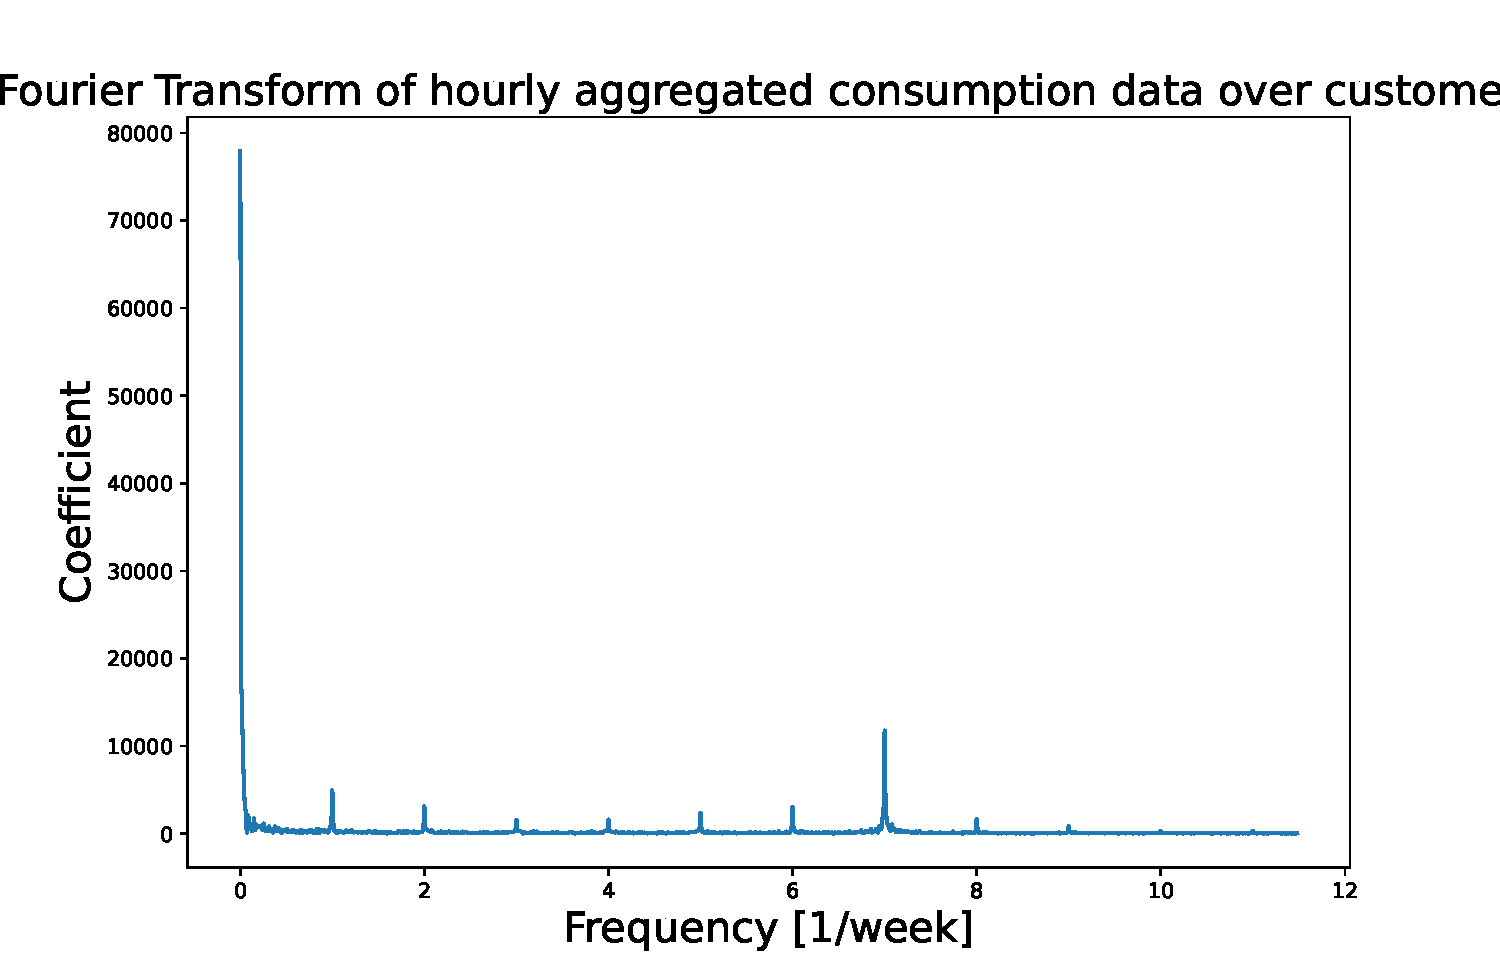
\includegraphics[width=0.4\textwidth]{images/demand/ft_hour_week}
\caption{The coefficients given by the Fourier transform for the hourly aggregated consumption over the customers.}
\label{fig:demandft}
\end{figure}

The daily aggregated consumption over the customers is reported in figure~\ref{fig:demanddataplotday}.
Aggregating the data on a daily basis, it is possible to more clearly observe the weekly pattern of consumption, which exhibits an increase on weekdays and a decrease on weekends.

\begin{figure}[H]
\centering
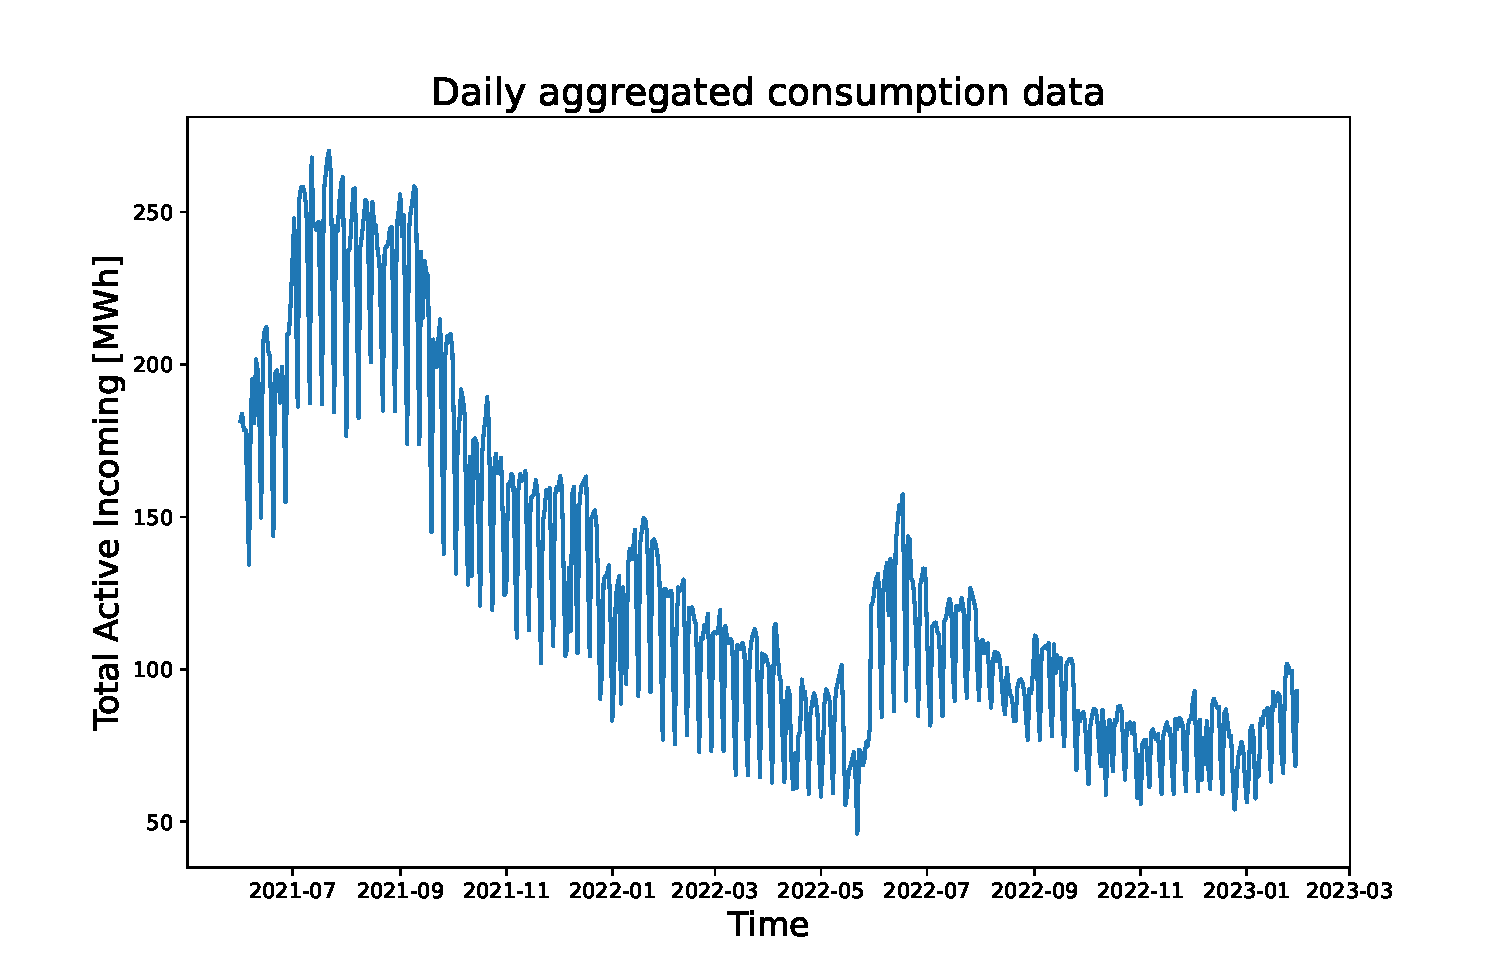
\includegraphics[width=0.5\textwidth]{images/demand/data_day_aggregated_plot}
\caption{The daily aggregated consumption over the customers.}
\label{fig:demanddataplotday}
\end{figure}

Figure~\ref{fig:demanddecompositionday} shows the time series decomposition of the daily aggregated consumption over the customers, using an additive model with a period of one week.
The decomposition is consistent with the hourly aggregated consumption over the customers.

\begin{figure}[H]
\centering
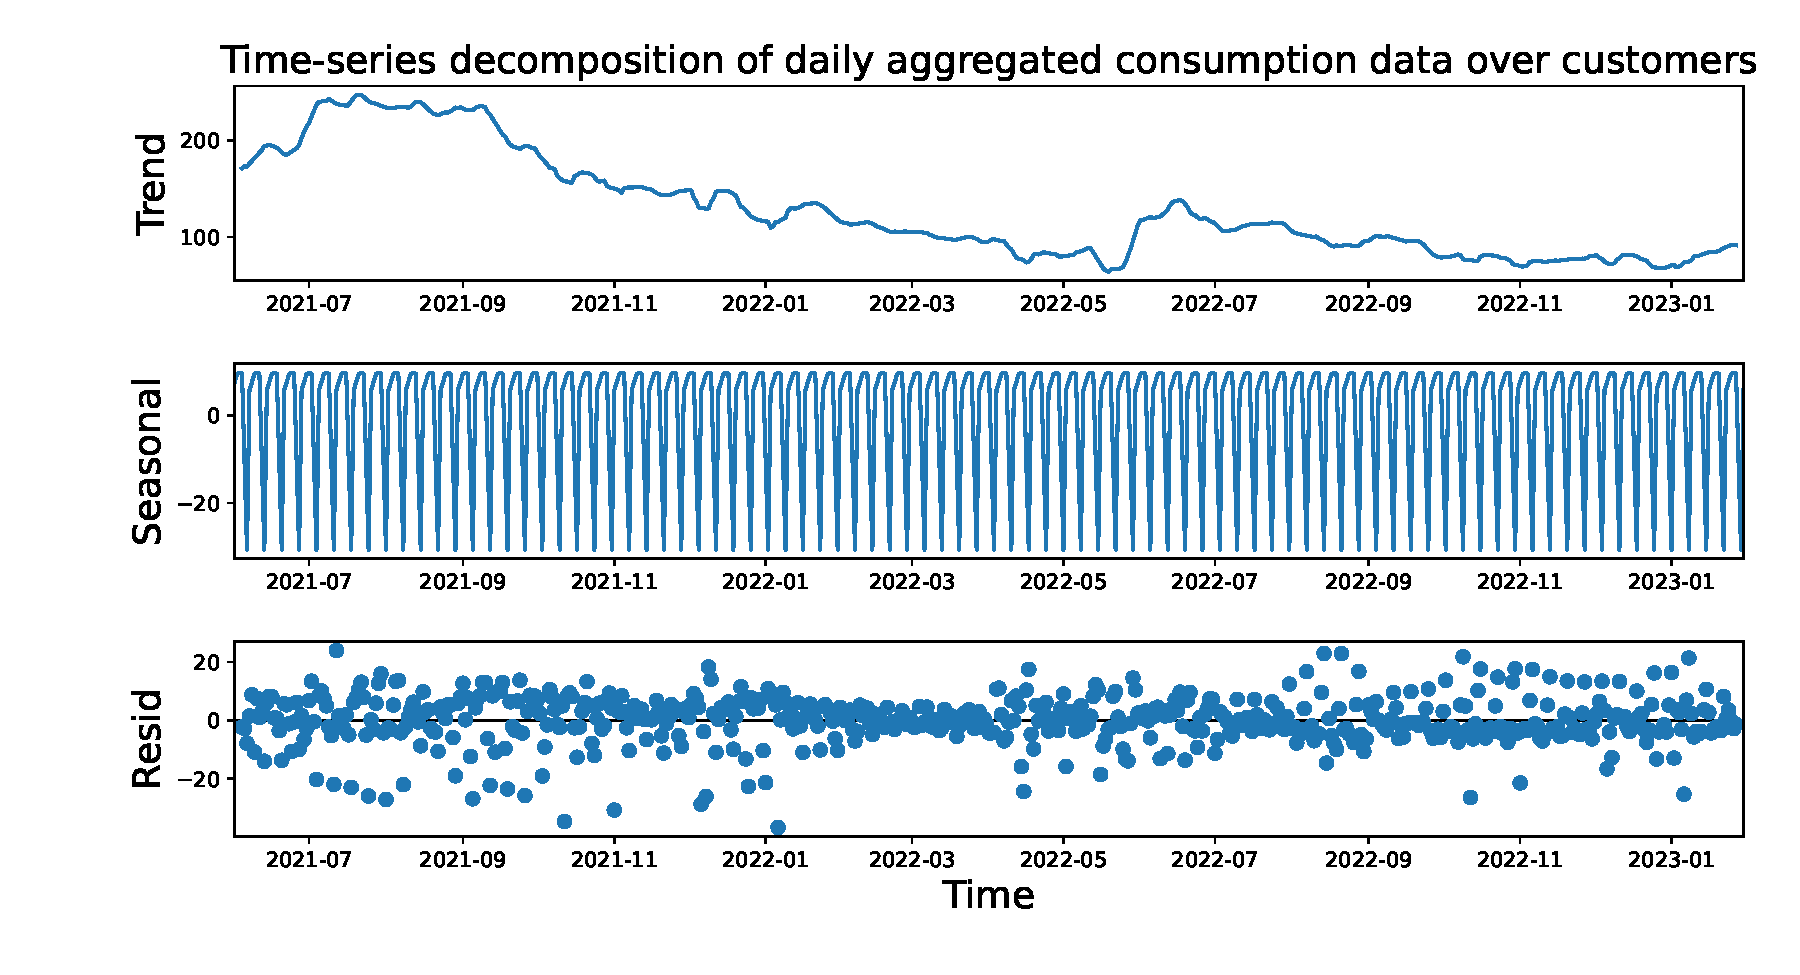
\includegraphics[width=0.5\textwidth]{images/demand/daily_aggregated_decomposition}
\caption{The time series decomposition of the daily aggregated consumption over the customers considering as period of the time series a week.}
\label{fig:demanddecompositionday}
\end{figure}

The auto-correlation of the daily aggregated consumption over the customers is reported in figure~\ref{fig:demandcorrelationday}.
It shows a high auto-correlation value in the closest time lag, with an even greater value at every week lag.
This suggests that useful features, since highly correlated, for predicting a time instant's demand may be the closest ones, but also those from the same day of the week in the previous weeks.
A good trade-off can be achieved by considering the consumption data in the previous 14 days.

\begin{figure}[H]
\centering
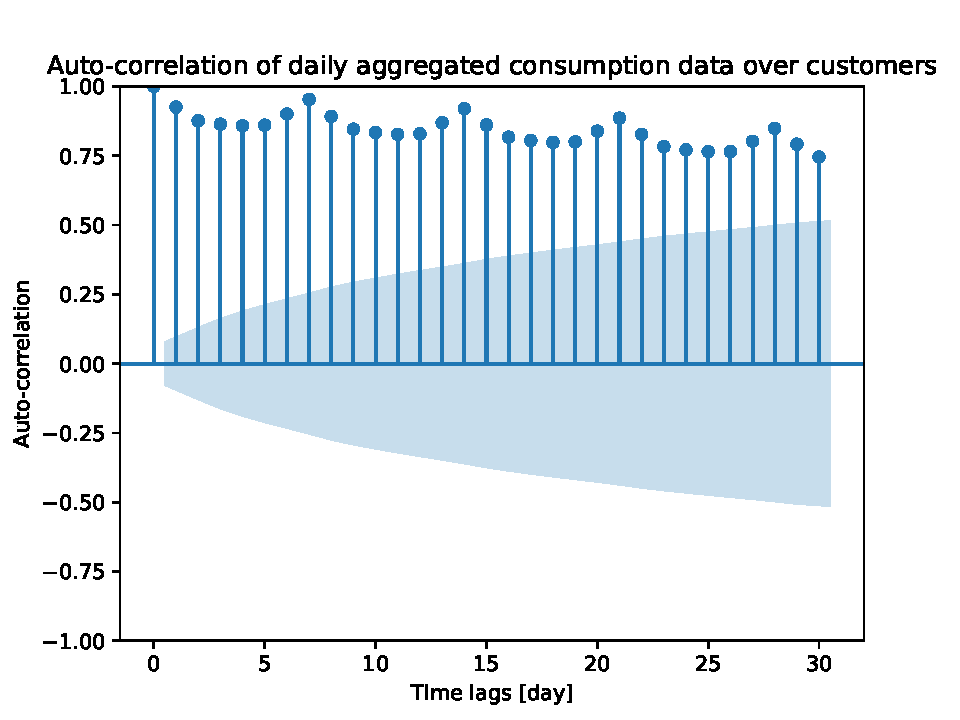
\includegraphics[width=0.4\textwidth]{images/demand/daily_aggregated_correlation}
\caption{The auto-correlation of the daily aggregated consumption over the customers.}
\label{fig:demandcorrelationday}
\end{figure}

The coefficients given by the Fourier transform for the daily aggregated consumption over the customers are reported in figure~\ref{fig:demandftday}.
The graphical representation shows 1 main frequency representing the weekly periodicity and other minor peaks at multiples of the 1/week frequency.

\begin{figure}[H]
\centering
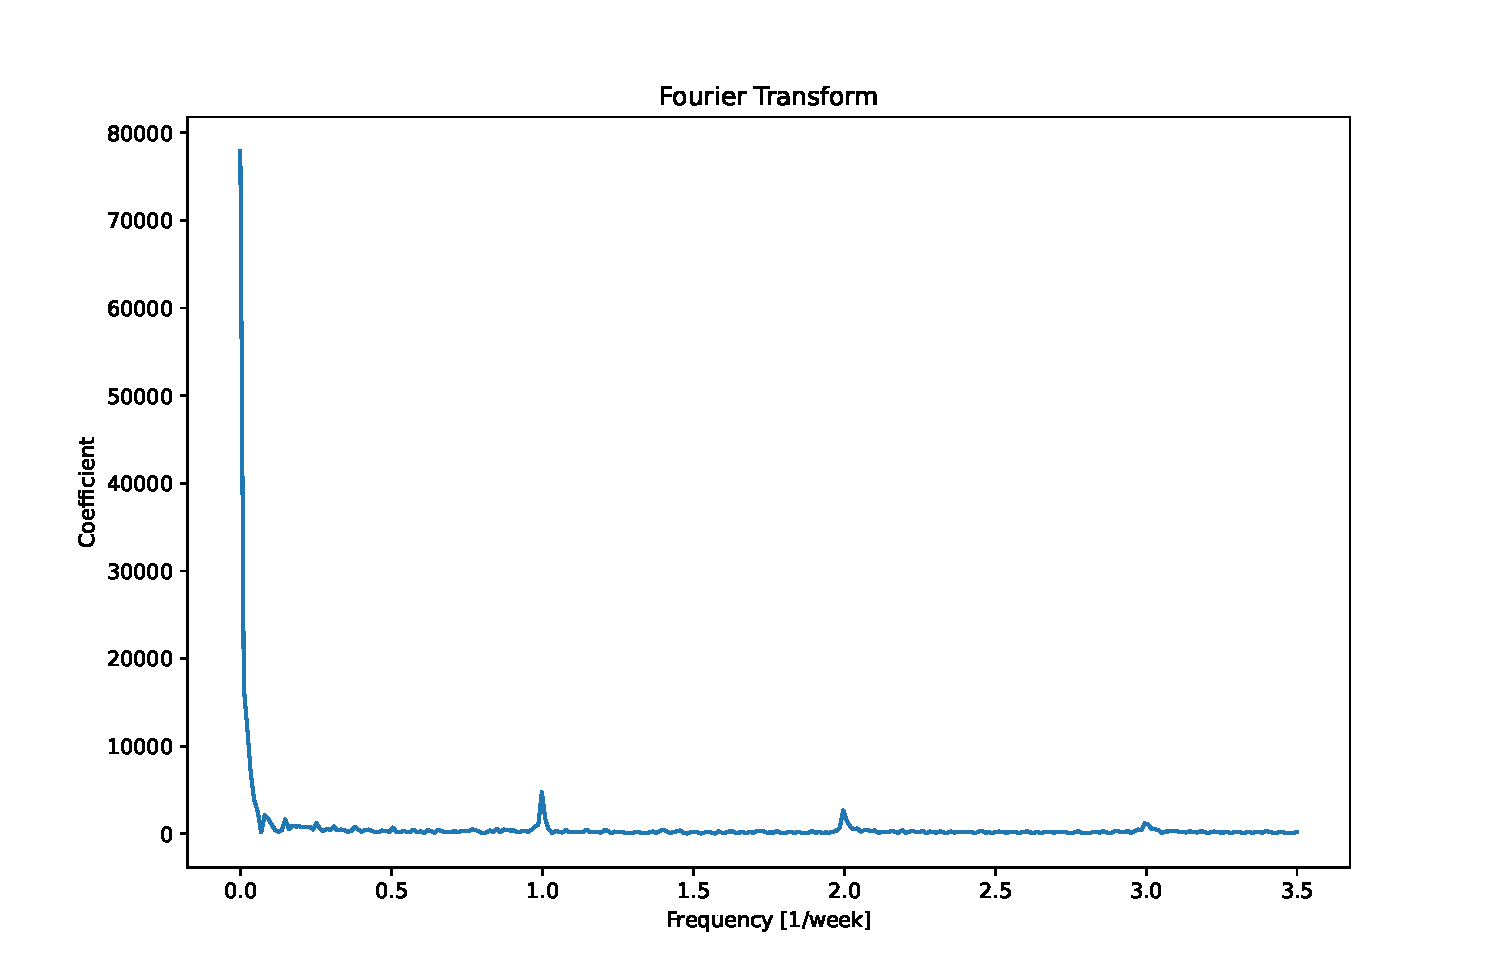
\includegraphics[width=0.4\textwidth]{images/demand/ft_day}
\caption{The coefficients given by the Fourier transform for the daily aggregated consumption over the customers.}
\label{fig:demandftday}
\end{figure}

Basic data is enhanced with the air temperature, the apparent temperature, and the relative humidity since they are considered the only weather features capable of influencing customers' energy consumption.
To assess the relationship between these weather variables and the aggregated consumption over the customers, two correlation coefficients were used: Pearson's correlation coefficient and Spearman's rank correlation coefficient.
Pearson's correlation coefficient measures the strength of the linear relationship between two variables, while Spearman's rank correlation coefficient measures the strength of the monotonic relationship.
The pearsonr and spearmanr methods of the SciPy library\footnote{ \url{https://scipy.org/} } were used to compute the correlation with weather data.
The results showed that the hourly aggregated consumption over the customers had:
\begin{itemize}
  \item a Pearson correlation coefficient of 0.4480 and a Spearman's rank correlation coefficient of 0.4378 with respect to the air temperature;
  \item a Pearson correlation coefficient of 0.4475 and a Spearman's rank correlation coefficient of 0.4368 with respect to the apparent temperature;
  \item a Pearson correlation coefficient of -0.2689 and a Spearman's rank correlation coefficient of -0.3173 with respect to the relative humidity.
\end{itemize}
It can be noticed that both the coefficients indicate a moderate correlation between the weather variables and consumption, this suggests that incorporating weather data into the prediction models could be useful.

The results showed that the daily aggregated consumption over the customers had:
\begin{itemize}
  \item a Pearson correlation coefficient of 0.3957 and a Spearman's rank correlation coefficient of 0.3156 with respect to the air temperature;
  \item a Pearson correlation coefficient of 0.3883 and a Spearman's rank correlation coefficient of 0.3155 with respect to the apparent temperature;
  \item a Pearson correlation coefficient of -0.0966 and a Spearman's rank correlation coefficient of -0.1582 with respect to the relative humidity.
\end{itemize}
It can be noticed that both the coefficients decreased considering the daily data meaning that the mean weather data over the day is less correlated to the daily aggregated consumption over the customers, compared to the hourly granularity.

Describe the choice of parameters for models ... (list with motivations)

Analyze the forecasts of the models for the electricity demand forecasting task (predictive analytics) ...
% TODO ancora da ultimare SARIMA o arima su serie equipollente e AutoML su altre granularità
12 splits were used for block validation with a test size of 720 each time.
Basically starting with 5977 entries and predicting every time 720 entries until reaching the last prediction instant where the model has a training size of 13897.

Summary table with results ...
% TODO where results are the one given by cross-validation mean ± std
% TODO check the consistency of model results in the last period and using cross-validation --> do a table with the differences (+ plot for internal analysis)
% TODO then add the comparison with forecasts of their provider
% commentarli (sia il numero che il grafico dell’errore) --> interpretare il dato (perchè è buono?) --> benchmark in letteratura, come va il loro, ecc…
% [valutare criticamente, aspetto tecnologico scientifico]


\section{Electricity production forecasting}
\label{sec:productionval}
\vspace{0.2 cm}

As described in the data preprocessing in chapter~\ref{cha:implementation}, single PV plant production data are aggregated to obtain the aggregated production data over the PV plants.
The target of the predictions is the mean percentage of production, which is calculated as the division of the total produced energy by the total power of the PV plants.
This allows us to have a bounded value from 0 to 100 from which it is possible to obtain the total produced energy simply by multiplying it by the total power of the PV plants.
This was also done since PV plants are added over time and this was unpredictable, this results in predicting the percentage of production of the PV plants.
This data is analyzed to get some descriptive analytics before finding adequate models to forecast the production.
The time series decomposition using an additive model of the hourly percentage of production considering as period of the time series a day is reported in figure~\ref{fig:productiondecomposition}.
It showed a considerable amount of noise, comparable to seasonality and trend in magnitude.
The trend component exhibits a clear peak during the summer season.
As expected, the seasonality component appears to have the most significant impact on the time series.

\begin{figure}[H]
\centering
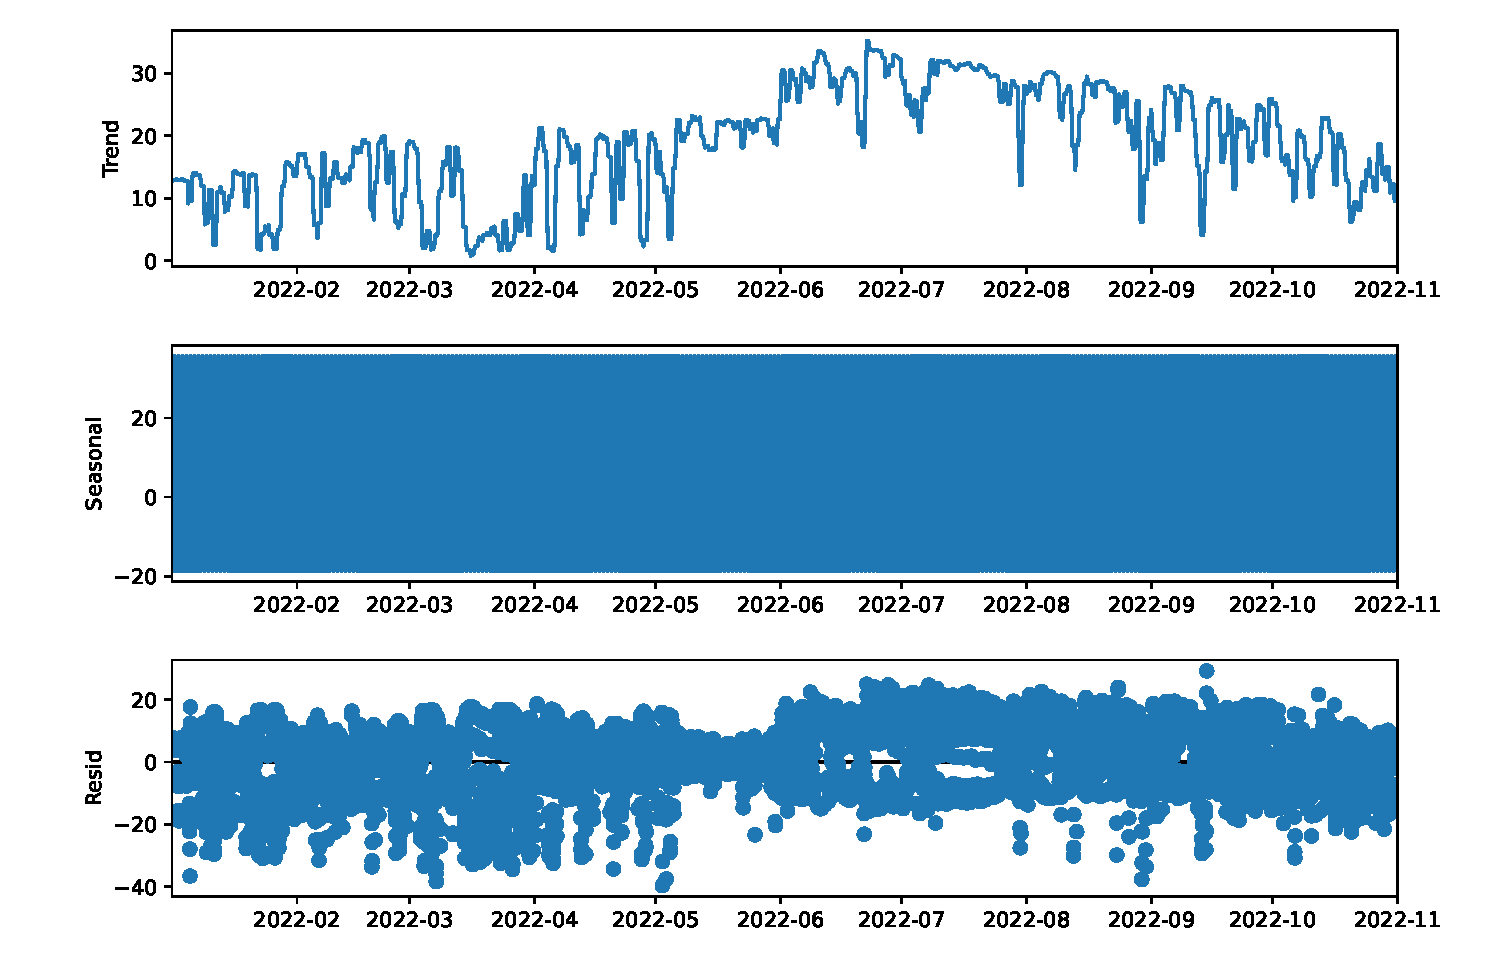
\includegraphics[width=0.5\textwidth]{images/production/hourly_decomposition}
\caption{The time series decomposition of the hourly percentage of production considering as period of the time series a day.}
\label{fig:productiondecomposition}
\end{figure}

The auto-correlation of the hourly percentage of production is reported in figure~\ref{fig:productioncorrelation}.
It shows a high auto-correlation value in the closest time lag and also at every 24 hours, with the value slightly decreasing as the lag increases over days.
This indicates that the production data from the closest time lag and those corresponding to the same hour in the preceding days may be valuable features for predicting a time instant's production.
A reasonable balance can be achieved by incorporating the production data up to the past 14 days.

\begin{figure}[H]
\centering
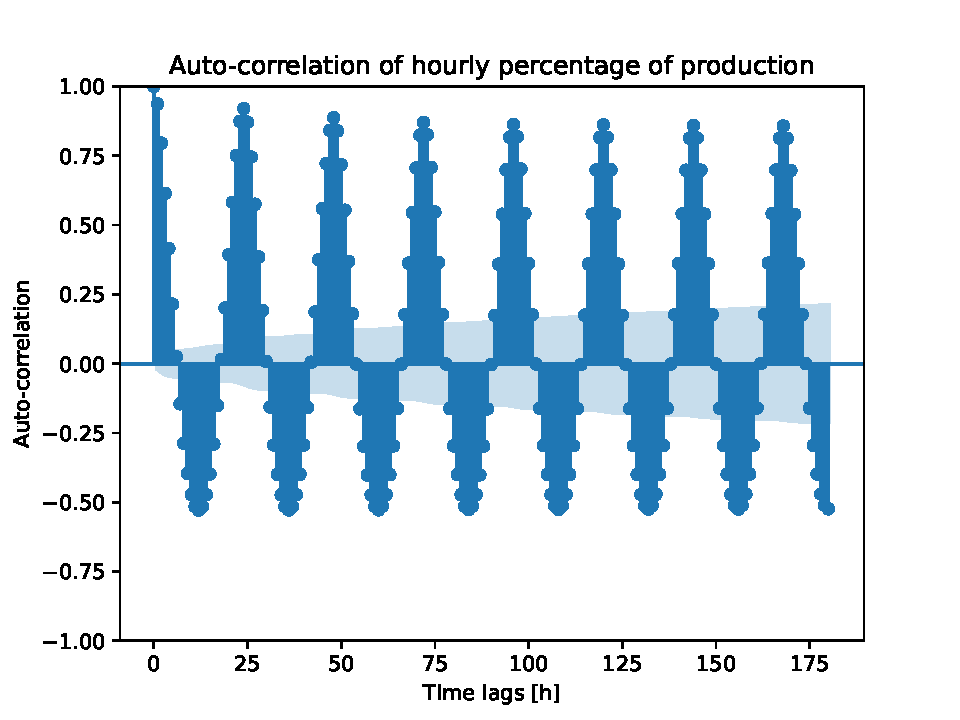
\includegraphics[width=0.4\textwidth]{images/production/hourly_correlation_week_range}
\caption{The auto-correlation of the hourly percentage of production.}
\label{fig:productioncorrelation}
\end{figure}

The coefficients given by the Fourier transform for the hourly percentage of production are reported in figure~\ref{fig:productionft}.
The graphical representation clearly shows a main frequency at the daily periodicity.
Other minor peaks are present mostly at multiples of the 1/day frequency.

\begin{figure}[H]
\centering
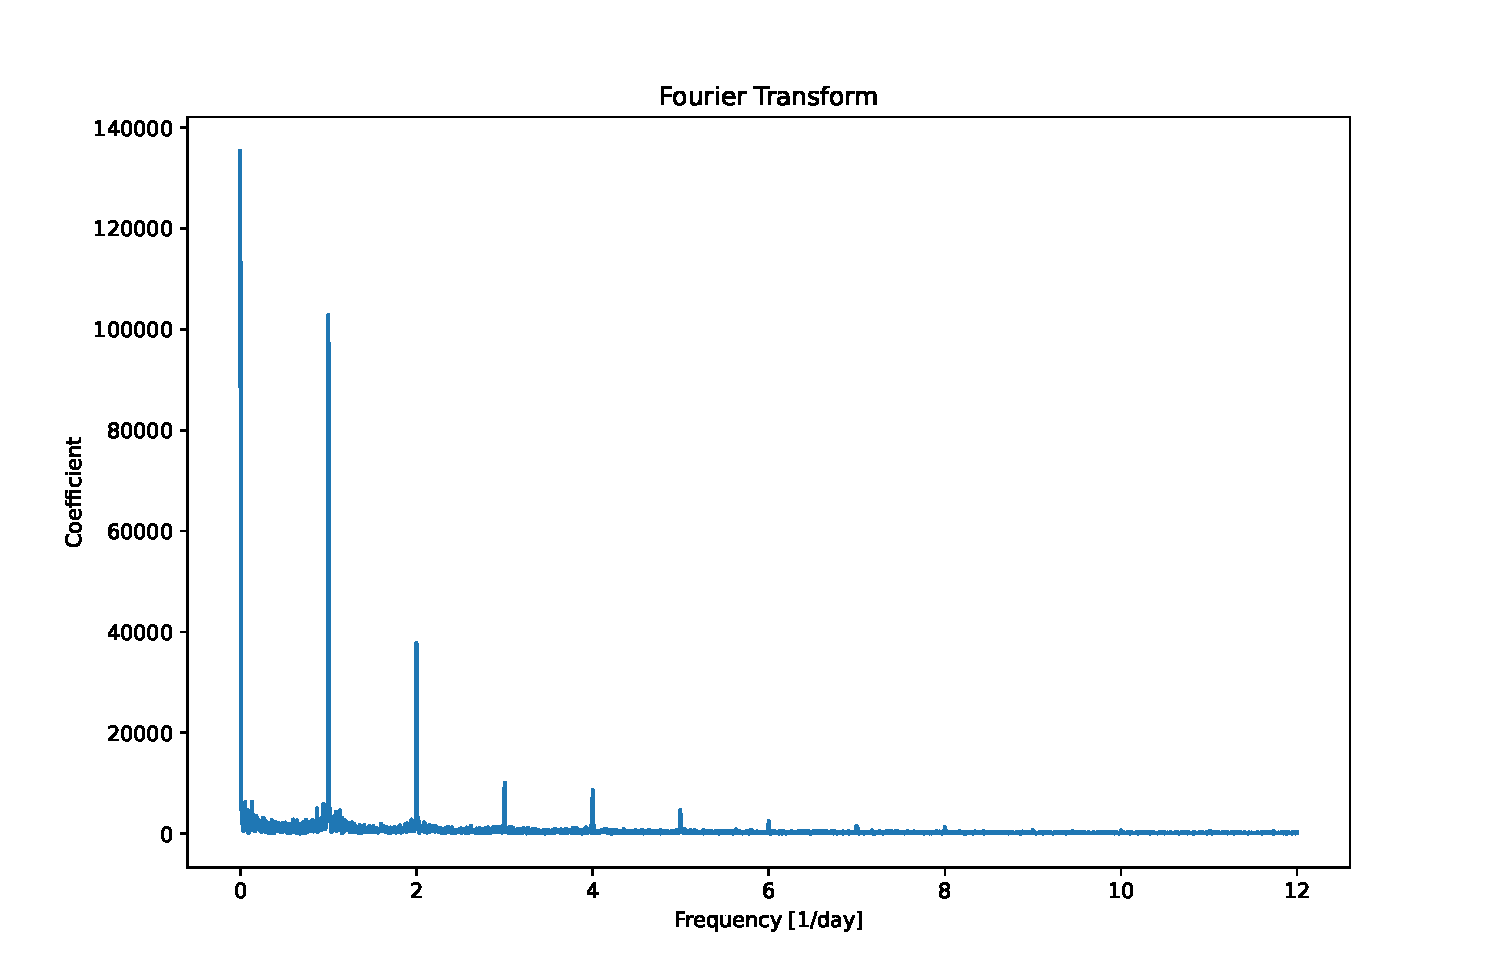
\includegraphics[width=0.4\textwidth]{images/production/ft_hour_day}
\caption{The coefficients given by the Fourier transform for the hourly percentage of production.}
\label{fig:productionft}
\end{figure}

The daily percentage of production is reported in figure~\ref{fig:productiondataplotday}.

\begin{figure}[H]
\centering
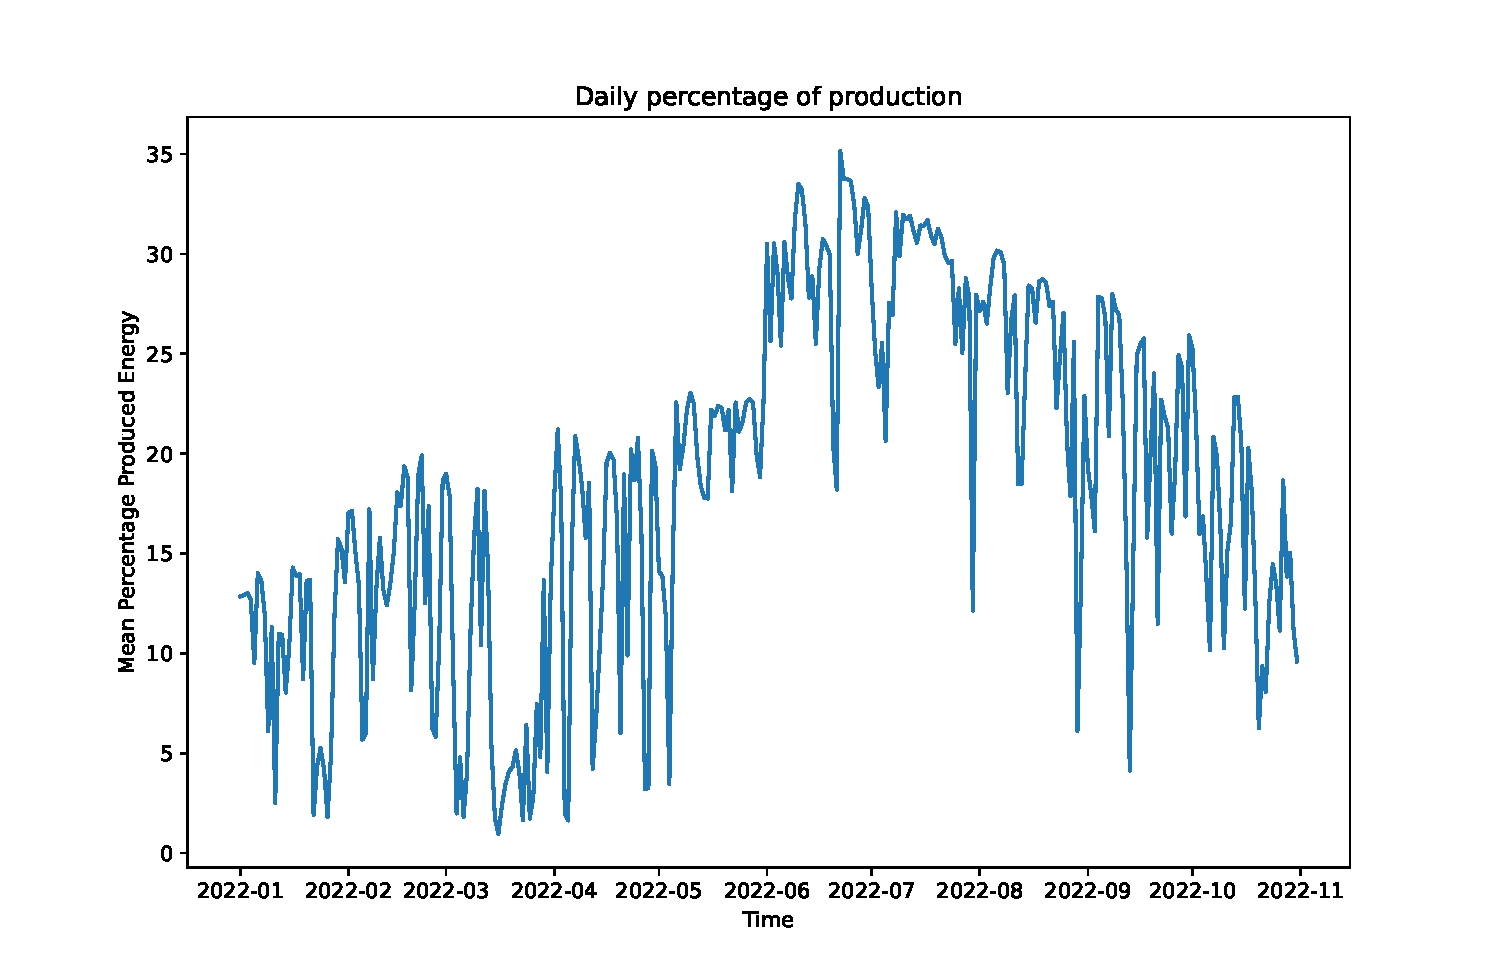
\includegraphics[width=0.5\textwidth]{images/production/data_day_aggregated_plot}
\caption{The daily percentage of production.}
\label{fig:productiondataplotday}
\end{figure}

The time series decomposition using an additive model of the daily percentage of production considering as period of the time series a week is reported in figure~\ref{fig:productiondecompositionday}.
It showed a considerable amount of noise, comparable to the trend in magnitude when not in the summer season.
The trend component exhibits a clear peak during the summer season and appears to be the significant component of the time series.
In this case, considering a weekly period, the seasonality component appears to not have a significant impact on the time series.

\begin{figure}[H]
\centering
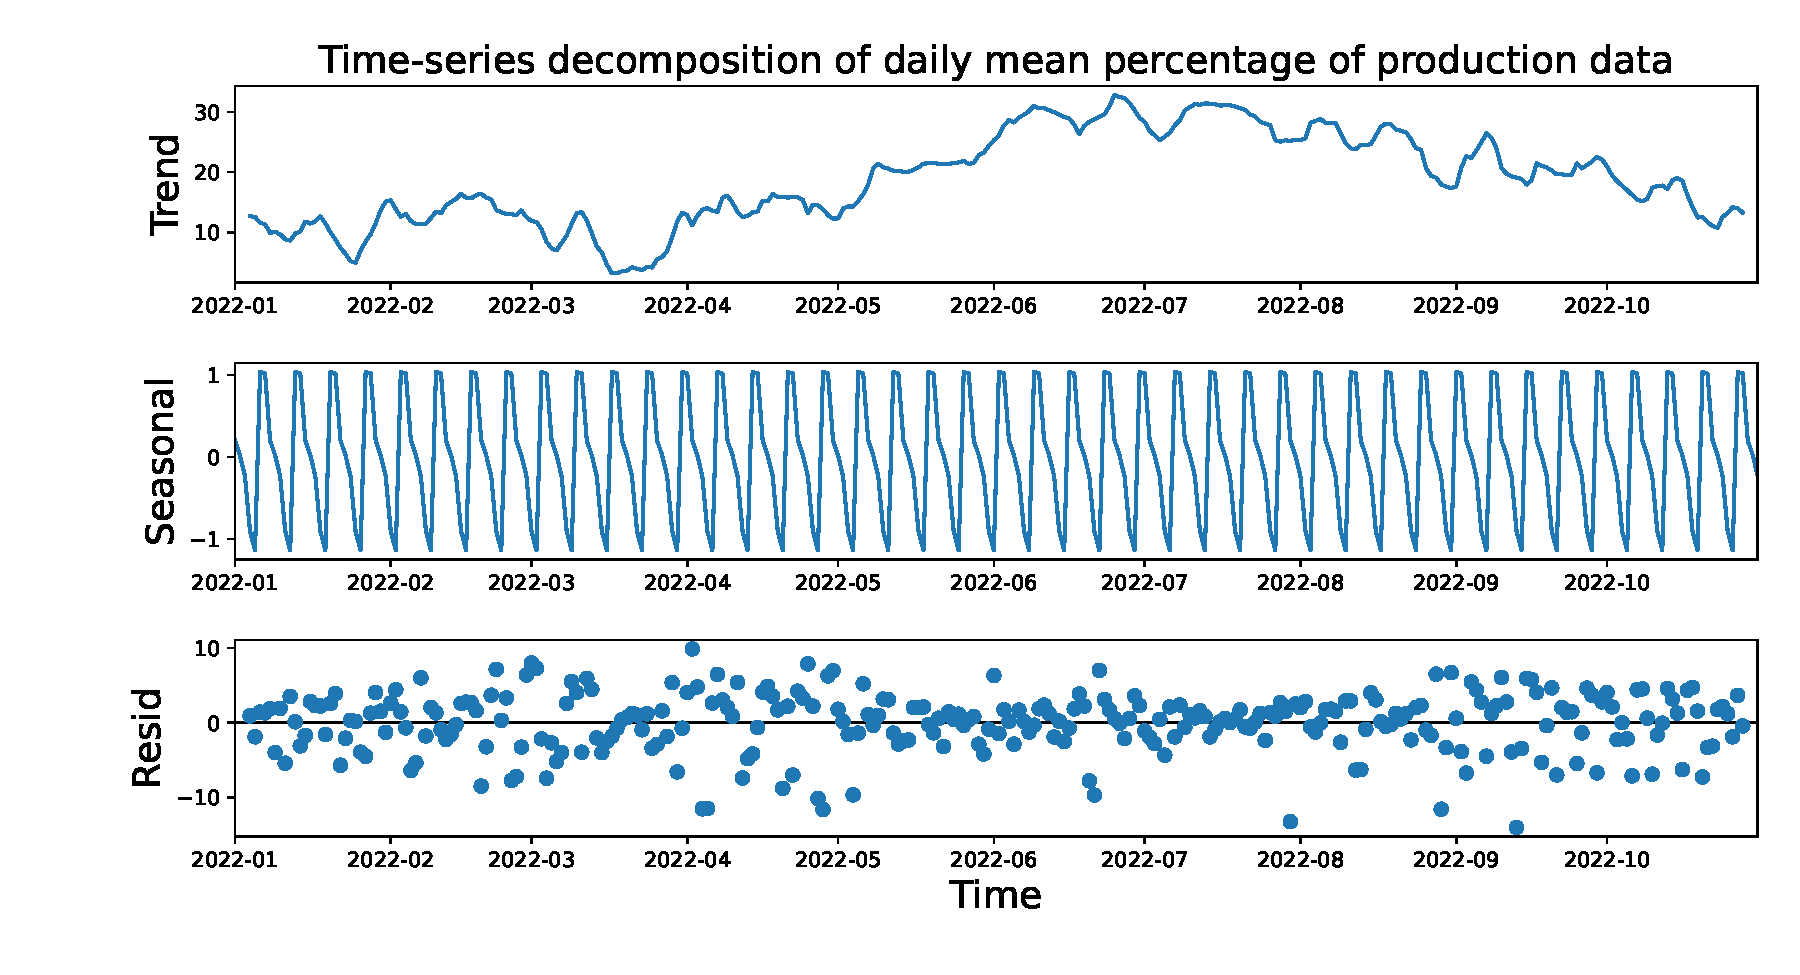
\includegraphics[width=0.5\textwidth]{images/production/daily_aggregated_decomposition}
\caption{The time series decomposition of the daily percentage of production considering as period of the time series a week.}
\label{fig:productiondecompositionday}
\end{figure}

The auto-correlation of the daily percentage of production is reported in figure~\ref{fig:productioncorrelationday}.
It shows a high auto-correlation value in the closest time lag and then a slight decrease as the lag increases over days.

\begin{figure}[H]
\centering
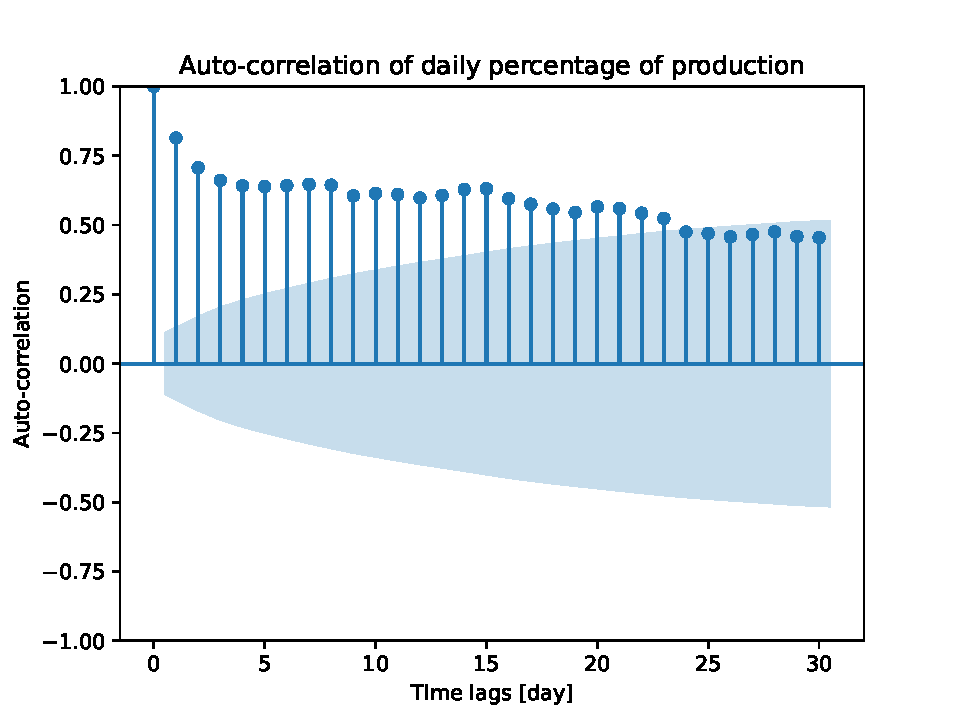
\includegraphics[width=0.4\textwidth]{images/production/daily_aggregated_correlation}
\caption{The auto-correlation of the daily percentage of production.}
\label{fig:productioncorrelationday}
\end{figure}

The coefficients given by the Fourier transform for the daily percentage of production are reported in figure~\ref{fig:productionftday}.
As expected from the time series decomposition, the graphical representation exhibits that there are no main frequencies in the daily percentage of production.

\begin{figure}[H]
\centering
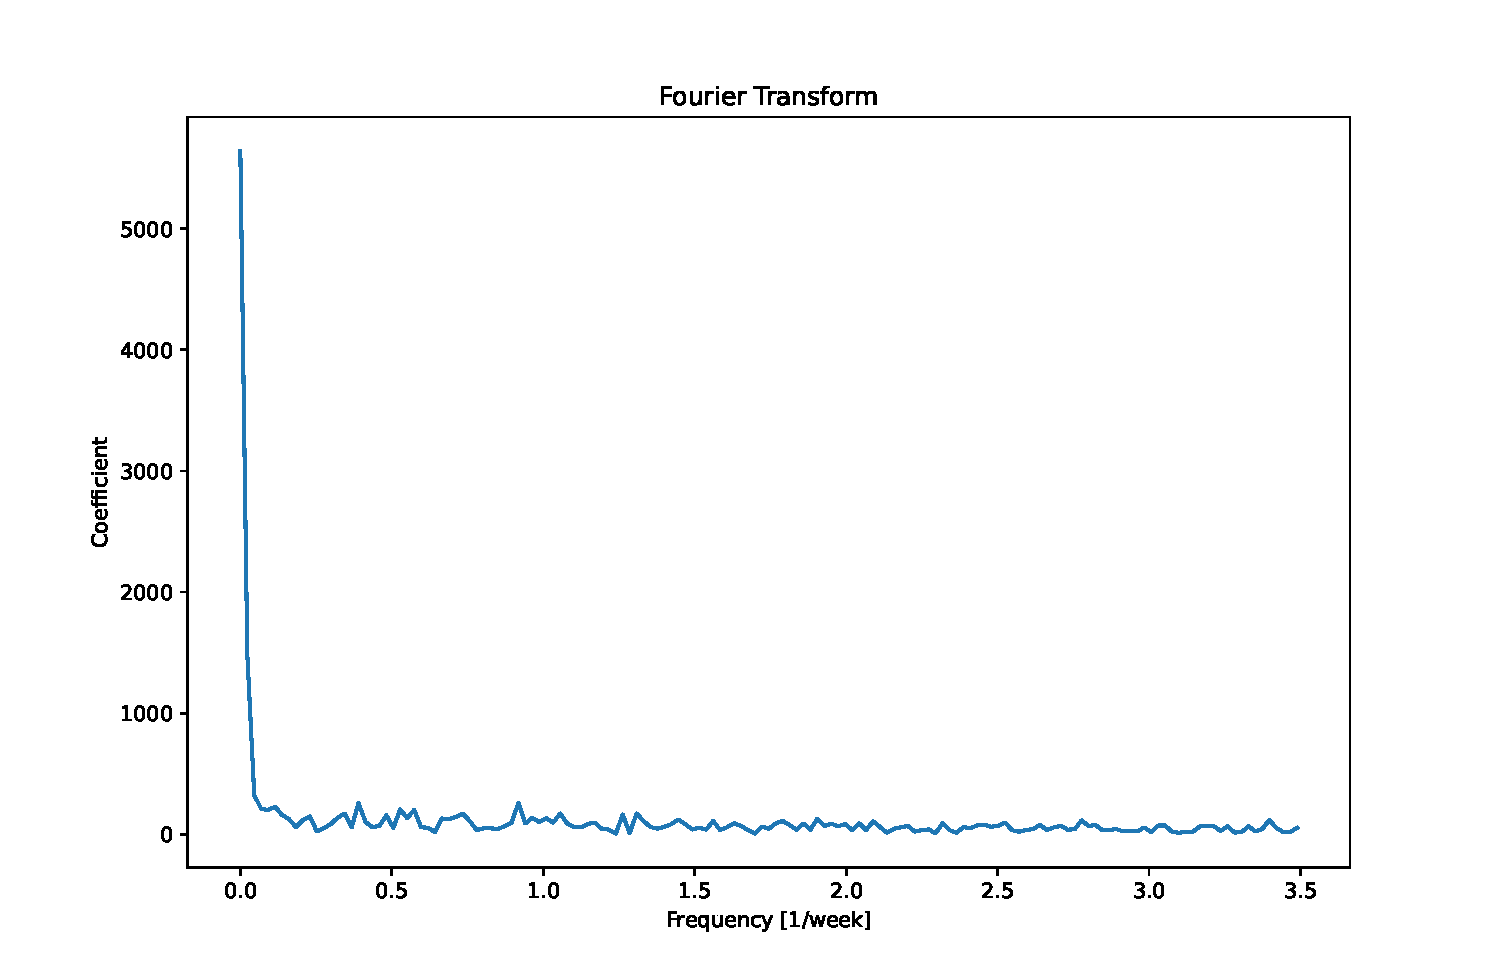
\includegraphics[width=0.4\textwidth]{images/production/ft_day}
\caption{The coefficients given by the Fourier transform for the daily percentage of production.}
\label{fig:productionftday}
\end{figure}

Basic data is enhanced with the air temperature, the apparent temperature, the relative humidity, the wind speed, the wind direction, the pressure altimeter, the visibility, the sky coverage, the diffuse horizontal irradiance, the direct normal irradiance, the global horizontal irradiance, the solar radiation, the UV index, the solar elevation angle, and the solar azimuth angle.
To assess the relationship between these weather variables and the percentage of production, two correlation coefficients were used: Pearson's correlation coefficient and Spearman's rank correlation coefficient.
Pearson's correlation coefficient measures the strength of the linear relationship between two variables, while Spearman's rank correlation coefficient measures the strength of the monotonic relationship.
The pearsonr and spearmanr methods of the SciPy library were used to compute the correlation with weather data.
The results showed that the hourly percentage of production had:
\begin{itemize}
  \item a Pearson correlation coefficient of 0.5621 and a Spearman's rank correlation coefficient of 0.5185 with respect to the air temperature;
  \item a Pearson correlation coefficient of 0.5410 and a Spearman's rank correlation coefficient of 0.5032 with respect to the apparent temperature;
  \item a Pearson correlation coefficient of -0.6318 and a Spearman's rank correlation coefficient of -0.5969 with respect to the relative humidity;
  \item a Pearson correlation coefficient of 0.3105 and a Spearman's rank correlation coefficient of 0.3237 with respect to the wind speed;
  \item a Pearson correlation coefficient of -0.1919 and a Spearman's rank correlation coefficient of -0.2155 with respect to the wind direction;
  \item a Pearson correlation coefficient of -0.2092 and a Spearman's rank correlation coefficient of -0.2645 with respect to the pressure altimeter;
  \item a Pearson correlation coefficient of -0.0132 and a Spearman's rank correlation coefficient of 0.0355 with respect to the visibility;
  \item a Pearson correlation coefficient of -0.2822 and a Spearman's rank correlation coefficient of -0.2375 with respect to the sky coverage;
  \item a Pearson correlation coefficient of 0.8559 and a Spearman's rank correlation coefficient of 0.9340 with respect to the diffuse horizontal irradiance;
  \item a Pearson correlation coefficient of 0.8399 and a Spearman's rank correlation coefficient of 0.9315 with respect to the direct normal irradiance;
  \item a Pearson correlation coefficient of 0.8791 and a Spearman's rank correlation coefficient of 0.9357 with respect to the global horizontal irradiance;
  \item a Pearson correlation coefficient of 0.9073 and a Spearman's rank correlation coefficient of 0.9472 with respect to the solar radiation;
  \item a Pearson correlation coefficient of 0.8571 and a Spearman's rank correlation coefficient of 0.9392 with respect to the UV index;
  \item a Pearson correlation coefficient of 0.8107 and a Spearman's rank correlation coefficient of 0.9057 with respect to the solar elevation angle;
  \item a Pearson correlation coefficient of 0.0450 and a Spearman's rank correlation coefficient of 0.0465 with respect to the solar azimuth angle.
\end{itemize}
It can be noticed that both the coefficients indicate a moderate to strong correlation between the hourly percentage of production and several weather features, including the air temperature, the apparent temperature, the relative humidity, the diffuse horizontal irradiance, the direct normal irradiance, the global horizontal irradiance, the solar radiation, the UV index, and the solar elevation angle.
Therefore, these features are chosen to be incorporated into the prediction models, while the other weather features show weaker correlations and are not considered.

The results showed that the daily percentage of production had:
\begin{itemize}
  \item a Pearson correlation coefficient of 0.7587 and a Spearman's rank correlation coefficient of 0.7701 with respect to the air temperature;
  \item a Pearson correlation coefficient of 0.7387 and a Spearman's rank correlation coefficient of 0.7451 with respect to the apparent temperature;
  \item a Pearson correlation coefficient of -0.7619 and a Spearman's rank correlation coefficient of -0.7501 with respect to the relative humidity;
  \item a Pearson correlation coefficient of 0.1874 and a Spearman's rank correlation coefficient of 0.3863 with respect to the wind speed;
  \item a Pearson correlation coefficient of -0.2384 and a Spearman's rank correlation coefficient of -0.2691 with respect to the wind direction;
  \item a Pearson correlation coefficient of -0.2525 and a Spearman's rank correlation coefficient of -0.2585 with respect to the pressure altimeter;
  \item a Pearson correlation coefficient of 0.2093 and a Spearman's rank correlation coefficient of 0.3096 with respect to the visibility;
  \item a Pearson correlation coefficient of -0.7081 and a Spearman's rank correlation coefficient of -0.6613 with respect to the sky coverage;
  \item a Pearson correlation coefficient of 0.6281 and a Spearman's rank correlation coefficient of 0.6968 with respect to the diffuse horizontal irradiance;
  \item a Pearson correlation coefficient of 0.6230 and a Spearman's rank correlation coefficient of 0.6952 with respect to the direct normal irradiance;
  \item a Pearson correlation coefficient of 0.6372 and a Spearman's rank correlation coefficient of 0.7016 with respect to the global horizontal irradiance;
  \item a Pearson correlation coefficient of 0.7912 and a Spearman's rank correlation coefficient of 0.8031 with respect to the solar radiation;
  \item a Pearson correlation coefficient of 0.8405 and a Spearman's rank correlation coefficient of 0.8693 with respect to the UV index;
  \item a Pearson correlation coefficient of 0.6499 and a Spearman's rank correlation coefficient of 0.7111 with respect to the solar elevation angle;
  \item a Pearson correlation coefficient of -0.0439 and a Spearman's rank correlation coefficient of 0.2738 with respect to the solar azimuth angle.
\end{itemize}
It can be noticed that both the coefficients decreased meaning that the mean weather data over the day is less correlated to the daily percentage of production, compared to the hourly granularity.
Only the hourly granularity is considered since PV plants are highly correlated with weather data and the aggregation over the day loses part of this correlation.

If we were forecasting the production of each PV plant individually, the weather data at the specific locations of the plants would result in a higher correlation with the production data and likely allow the models to produce more accurate forecasts.
However, since we are aggregating the production from multiple PV plants and looking for the overall percentage of production in the hour, using the weather data from a location located in the middle of the PV plants is also acceptable.
In figure~\ref{fig:pvplantsmap}, the locations of the PV plants and of the weather station are reported.

\begin{figure}[H]
\centering
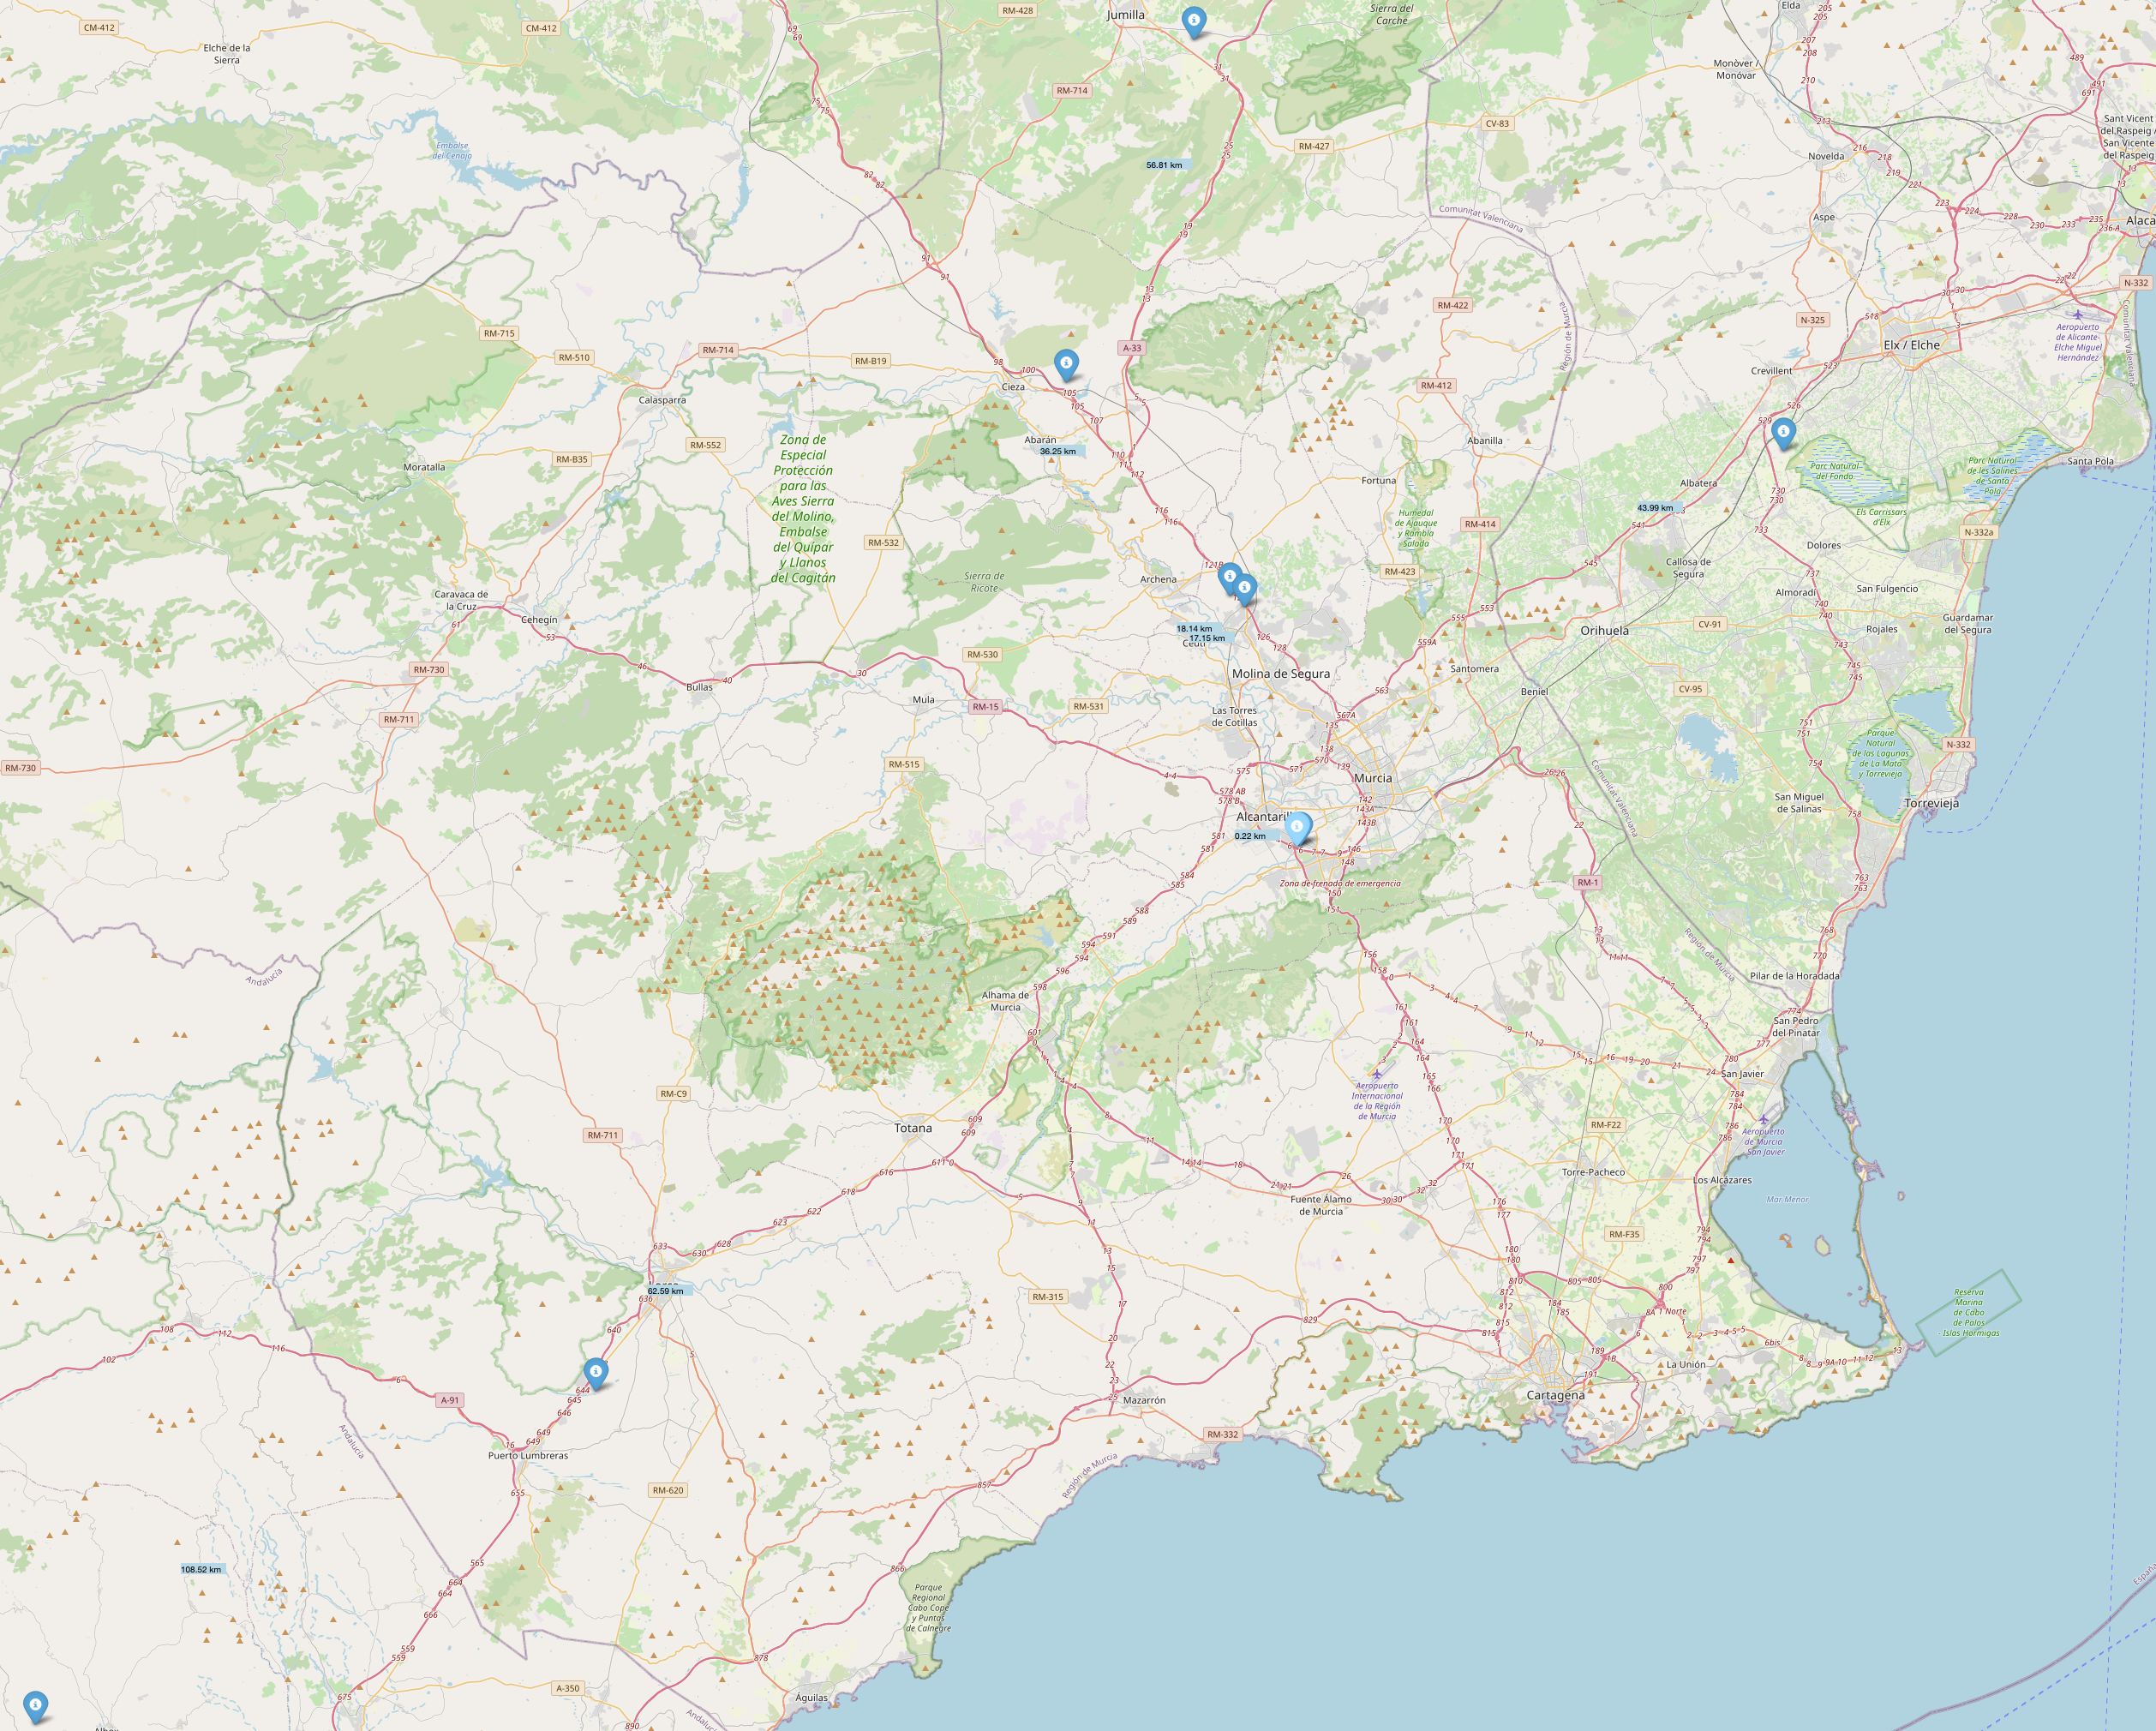
\includegraphics[width=0.8\textwidth]{images/production/pv_plants_map}
\caption{The map of the city of Murcia with indicated the location of the PV plants with a blue icon and of the revelation station with a lightblue icon. The distances between each PV plant and the weather station are reported in lightblue boxes near the PV plant locations.}
\label{fig:pvplantsmap}
\end{figure}

Describe the choice of parameters for models ... (list with motivations)

Analyze the forecasts of the models for the electricity production forecasting task (predictive analytics) ...
% TODO ancora da ultimare SARIMA o arima su serie equipollente e AutoML su altre granularità
12 splits were used for block validation with a test size of 168 each time.
Basically starting with 5280 entries and predicting every time 168 entries until reaching the last prediction instant where the model has a training size of 7128. % TODO

Summary table with results ...
% TODO where results are the one given by cross-validation mean ± std
% TODO check the consistency of model results in the last period and using cross-validation --> do a table with the differences (+ plot for internal analysis)
% TODO then add the comparison with forecasts of their provider
% commentarli (sia il numero che il grafico dell’errore) --> interpretare il dato (perchè è buono?) --> benchmark in letteratura, come va il loro, ecc…
% [valutare criticamente, aspetto tecnologico scientifico]


\section{Consumption baseline forecasting} 
\label{sec:baselineval}
\vspace{0.2 cm}

The consumption data of the three customers are analyzed to get some descriptive analytics before finding adequate models to forecast the consumption baseline of each customer.
The time series decompositions using an additive model of the hourly consumption of the three customers considering as period of the time series a week are reported in figure~\ref{fig:decompositioncustomer1}, figure~\ref{fig:decompositioncustomer2}, and figure~\ref{fig:decompositioncustomer3}.
All three decompositions show a considerable amount of noise, which is dominant in magnitude compared to the trend and seasonality.
For all the customers the seasonal component appears to not have a significant impact on the time series, with the exception of the second customer for which it is twice high in magnitude with respect to the others.
The trend component has a slight impact, for the first customer it is possible to see a peak in the winter, for the second customer it is present a peak in April, and for the third customer has not a clear trend.

\begin{figure}[H]
\begin{minipage}[b]{8.5cm}
\centering
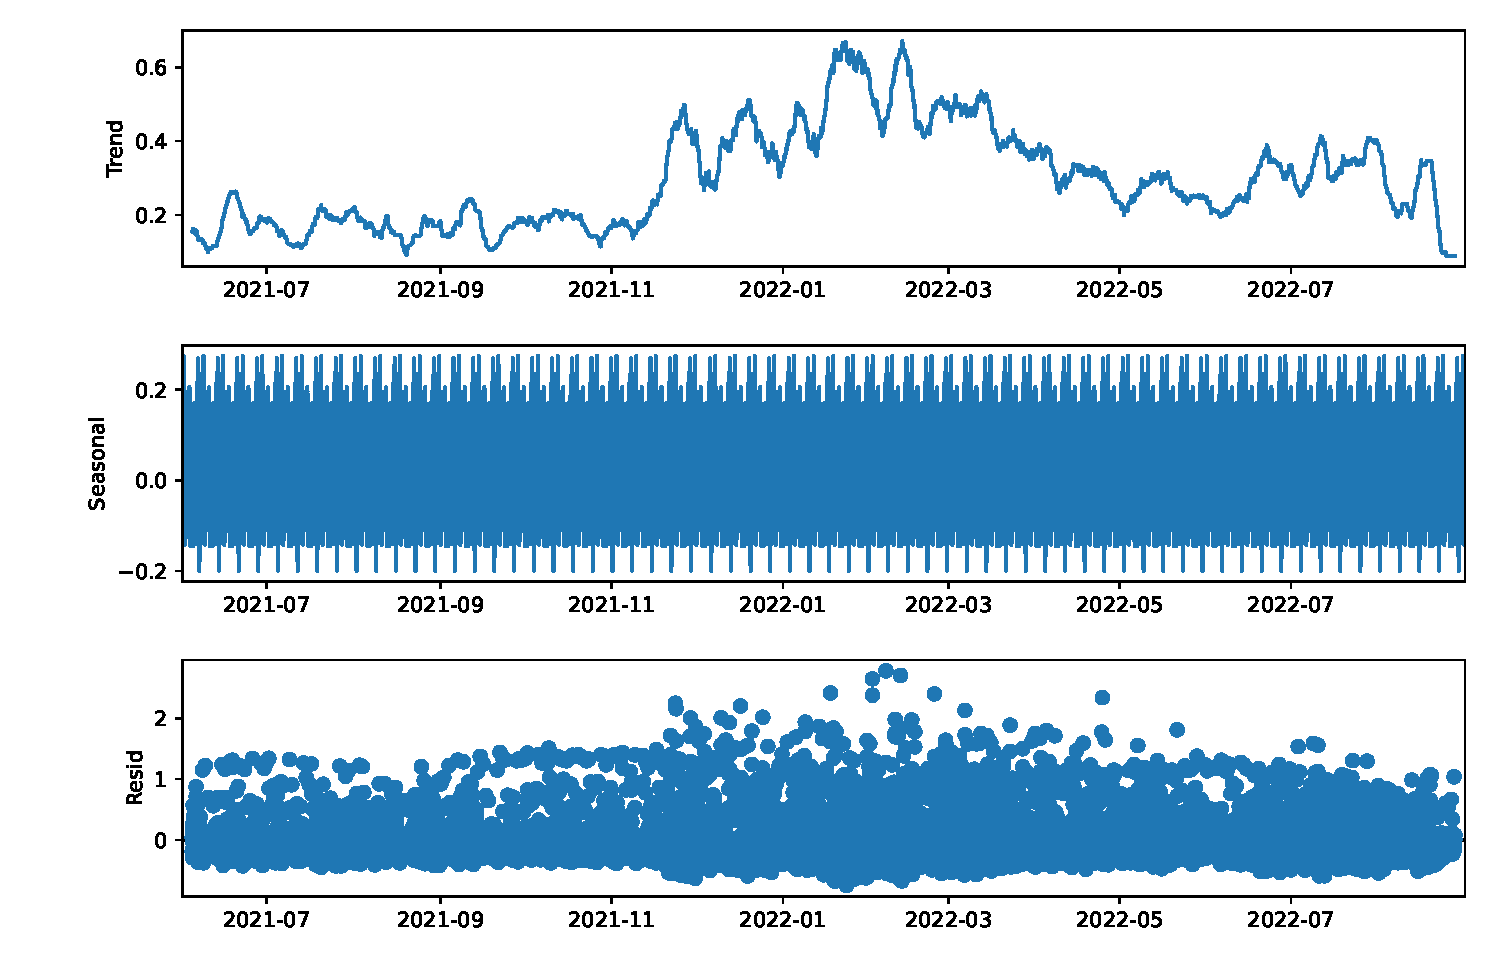
\includegraphics[width=1\textwidth]{images/baseline/hourly_decomposition_week_period_customer1}
\subcaption{First customer.}
\label{fig:decompositioncustomer1}
\end{minipage}
\ \hspace{2mm} \
\begin{minipage}[b]{8.5cm}
\centering
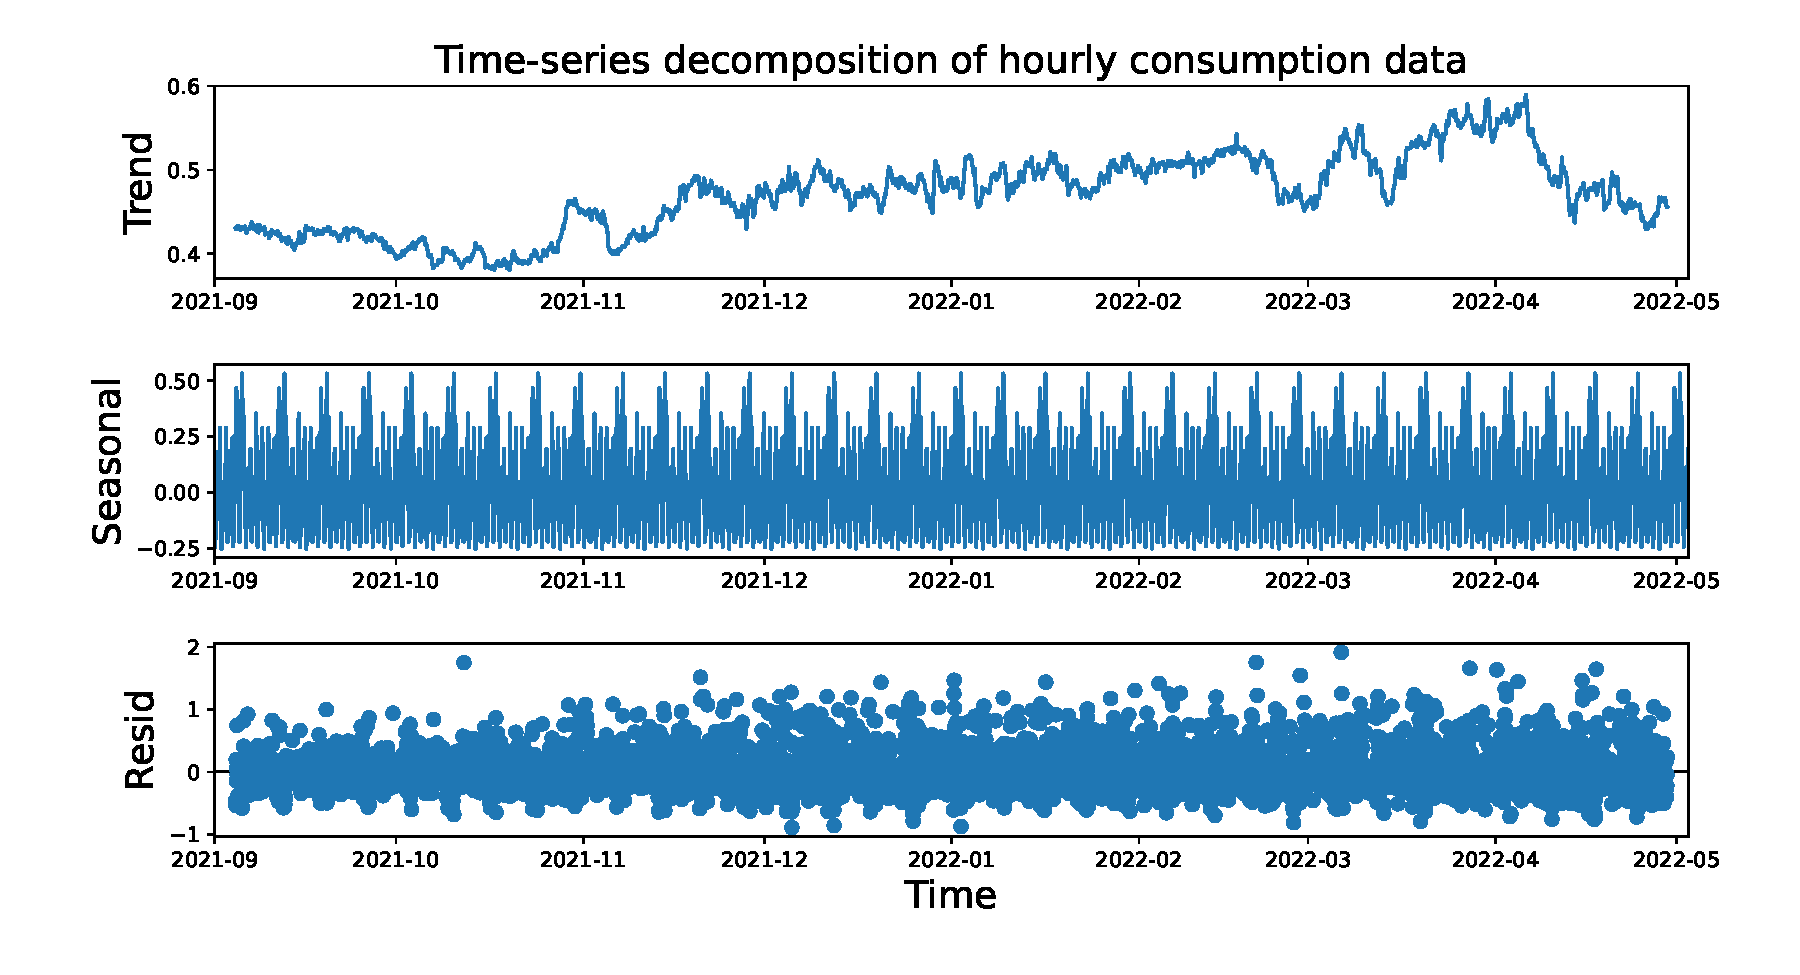
\includegraphics[width=1\textwidth]{images/baseline/hourly_decomposition_week_period_customer2}
\subcaption{Second customer.}
\label{fig:decompositioncustomer2}
\end{minipage}
\begin{minipage}[b]{17cm}
\centering
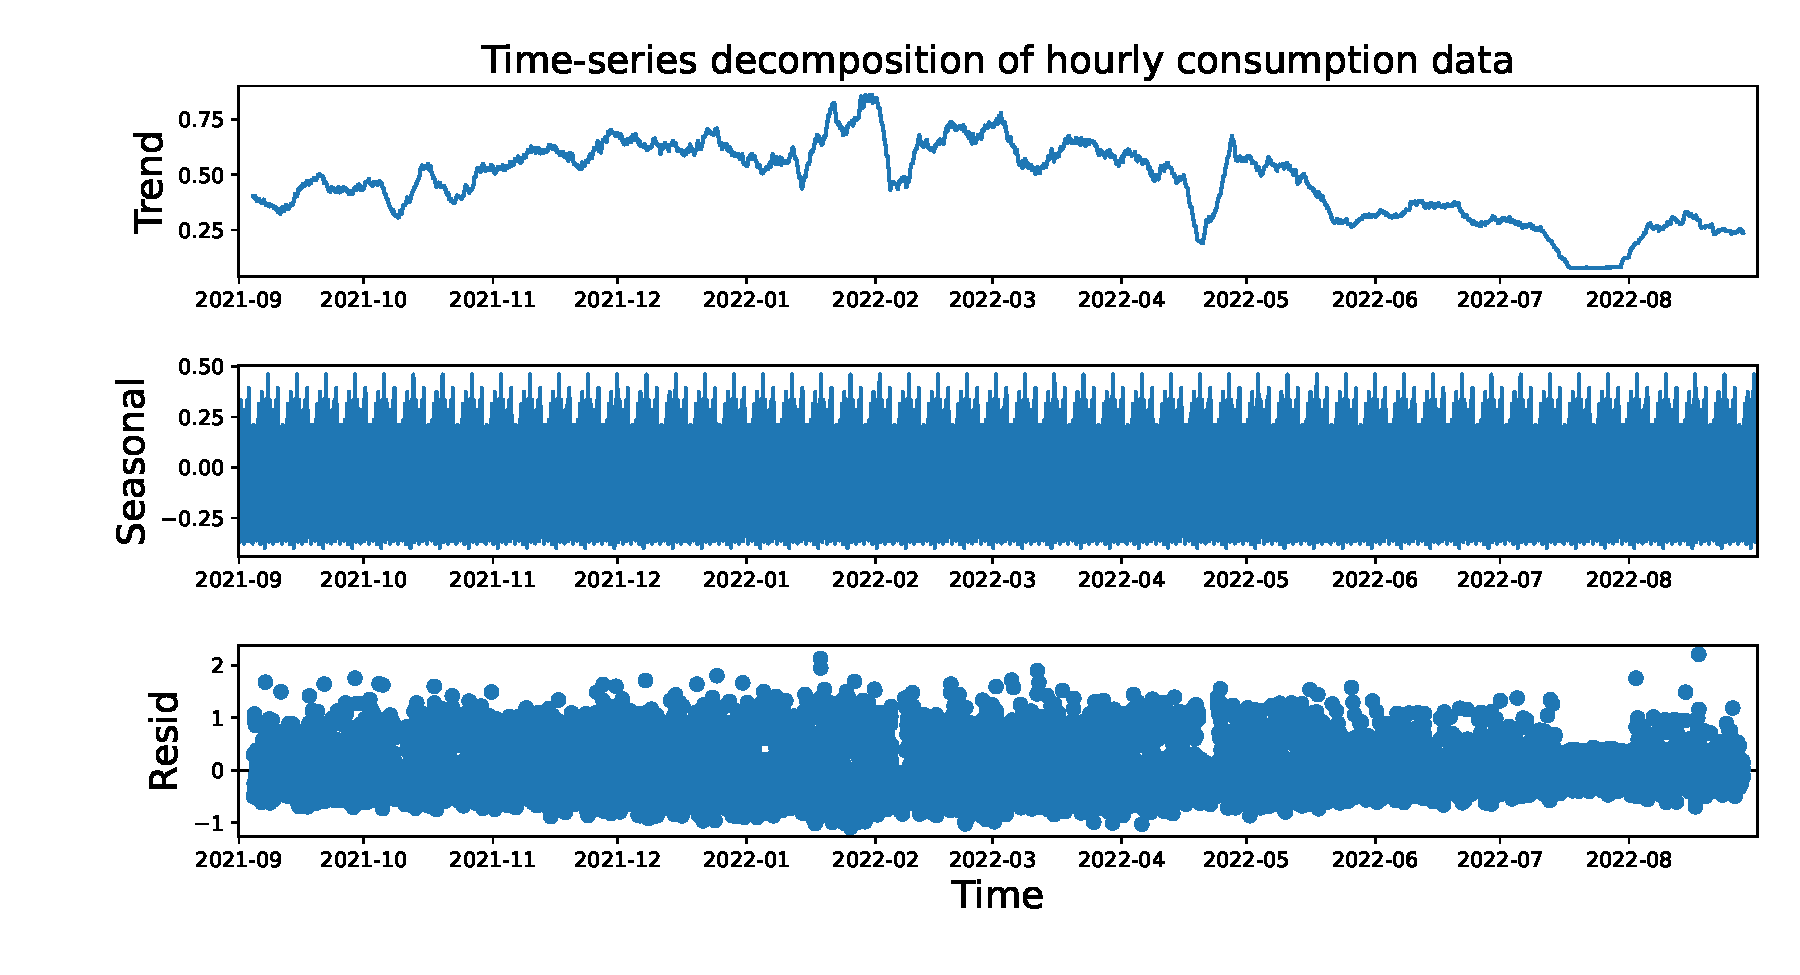
\includegraphics[width=0.5\textwidth]{images/baseline/hourly_decomposition_week_period_customer3}
\subcaption{Third customer.}
\label{fig:decompositioncustomer3}
\end{minipage}
\caption{The time series decompositions of the hourly consumption of the three customers considering as period of the time series a week.}
\end{figure}

The auto-correlations of the hourly consumption of the three customers are reported in figure~\ref{fig:correlationcustomer1}, figure~\ref{fig:correlationcustomer2}, and figure~\ref{fig:correlationcustomer3}.
All the customers’ consumptions are not very auto-correlated, it can be shown that the maximum auto-correlation value is around 0.5 in the closest time lag and that there is a peak every 24 hours, with a slightly greater value at one week distance.
This indicates that the consumption data from the closest time lag, as well as those corresponding to the same hour in the preceding days and even better in the preceding weeks, may be valuable features for predicting a time instant's demand.
A reasonable balance can be achieved by incorporating the consumption data up to the past 14 days.

The coefficients given by the Fourier transform for the hourly consumption of the three customers are reported in figure~\ref{fig:ftcustomer1}, figure~\ref{fig:ftcustomer2}, and figure~\ref{fig:ftcustomer3}.
The graphical representations show for all the customers a main frequency at the daily periodicity.
Other minor peaks are present mostly at multiples of the 1/day frequency, in particular for the third customer where the 2/day frequency is almost equal to the 1/day.

\begin{figure}[H]
\begin{minipage}[b]{8.5cm}
\centering
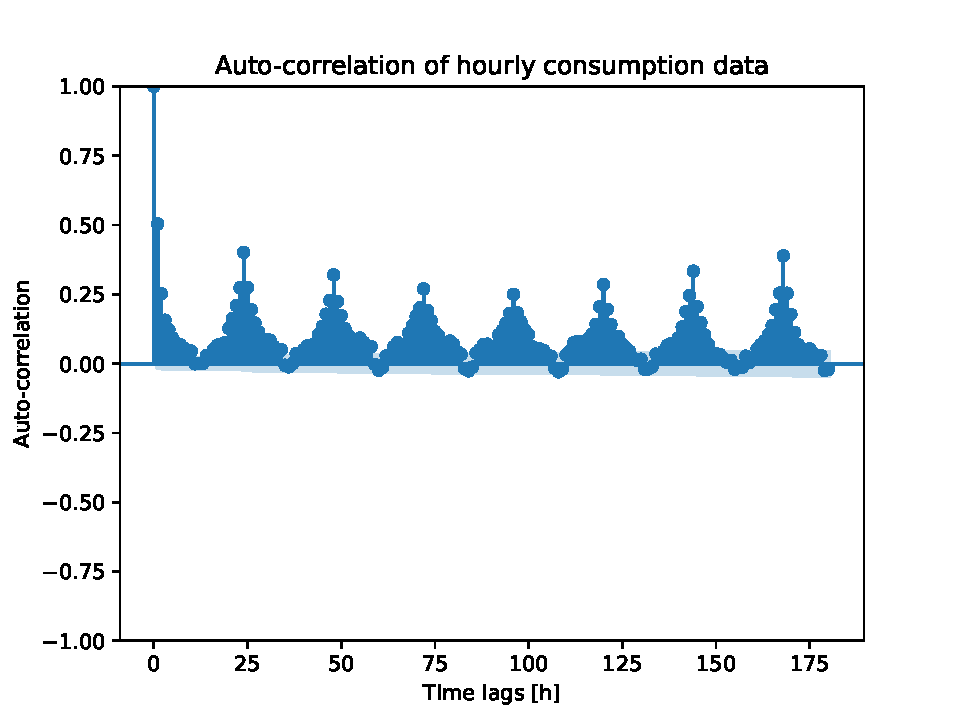
\includegraphics[width=0.8\textwidth]{images/baseline/hourly_correlation_week_range_customer1}
\subcaption{First customer.}
\label{fig:correlationcustomer1}
\end{minipage}
\ \hspace{2mm} \
\begin{minipage}[b]{8.5cm}
\centering
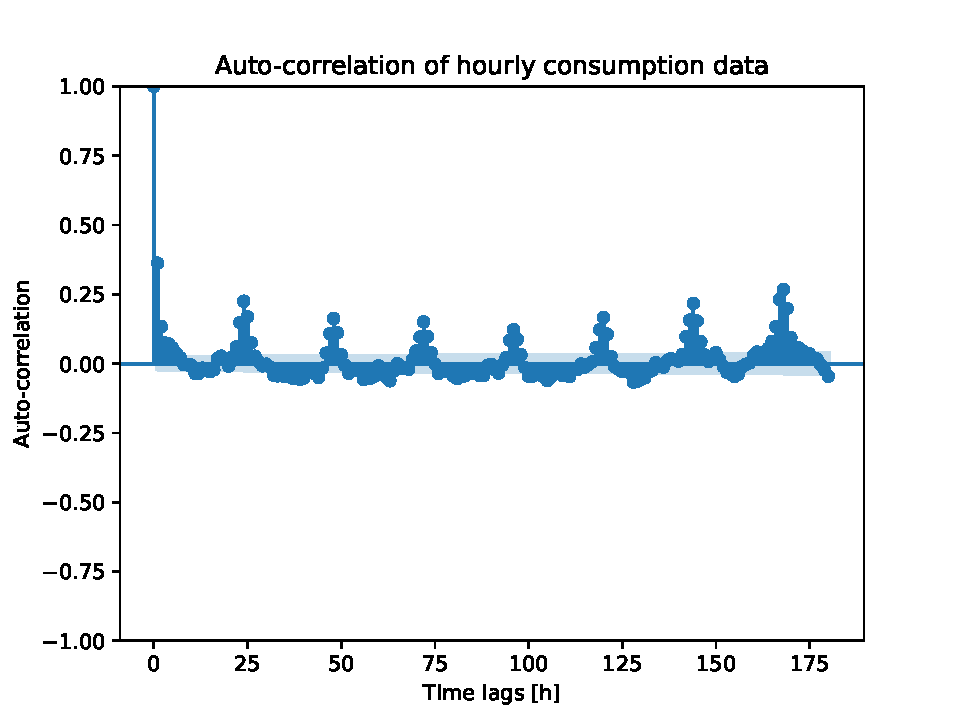
\includegraphics[width=0.8\textwidth]{images/baseline/hourly_correlation_week_range_customer2}
\subcaption{Second customer.}
\label{fig:correlationcustomer2}
\end{minipage}
\begin{minipage}[b]{17cm}
\centering
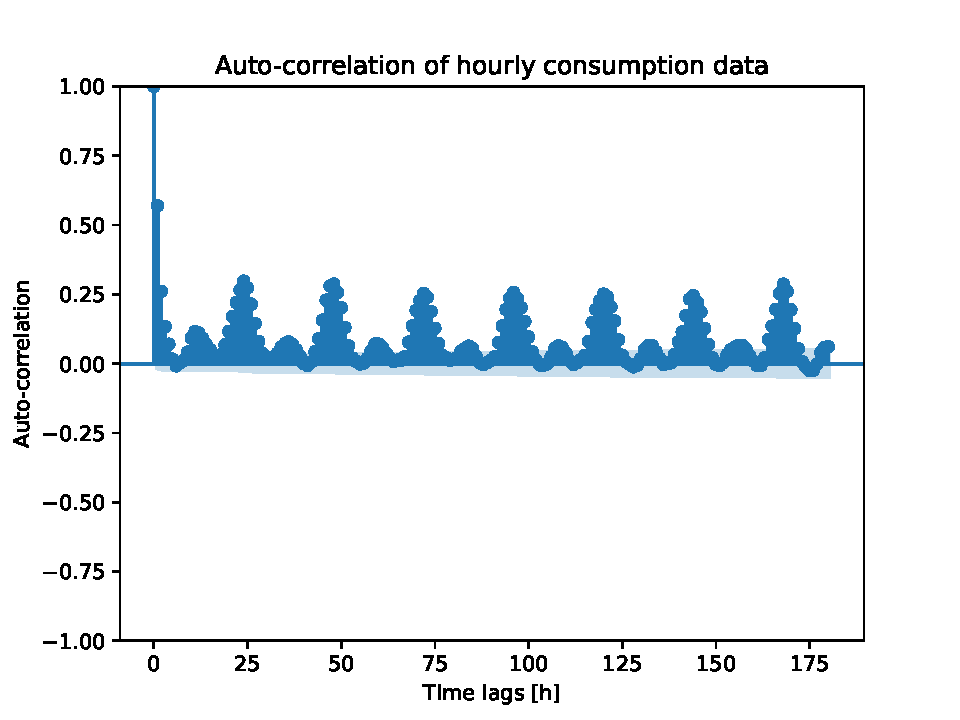
\includegraphics[width=0.4\textwidth]{images/baseline/hourly_correlation_week_range_customer3}
\subcaption{Third customer.}
\label{fig:correlationcustomer3}
\end{minipage}
\caption{The auto-correlations of the hourly consumption of the three customers.}
\end{figure}

\begin{figure}[H]
\begin{minipage}[b]{8.5cm}
\centering
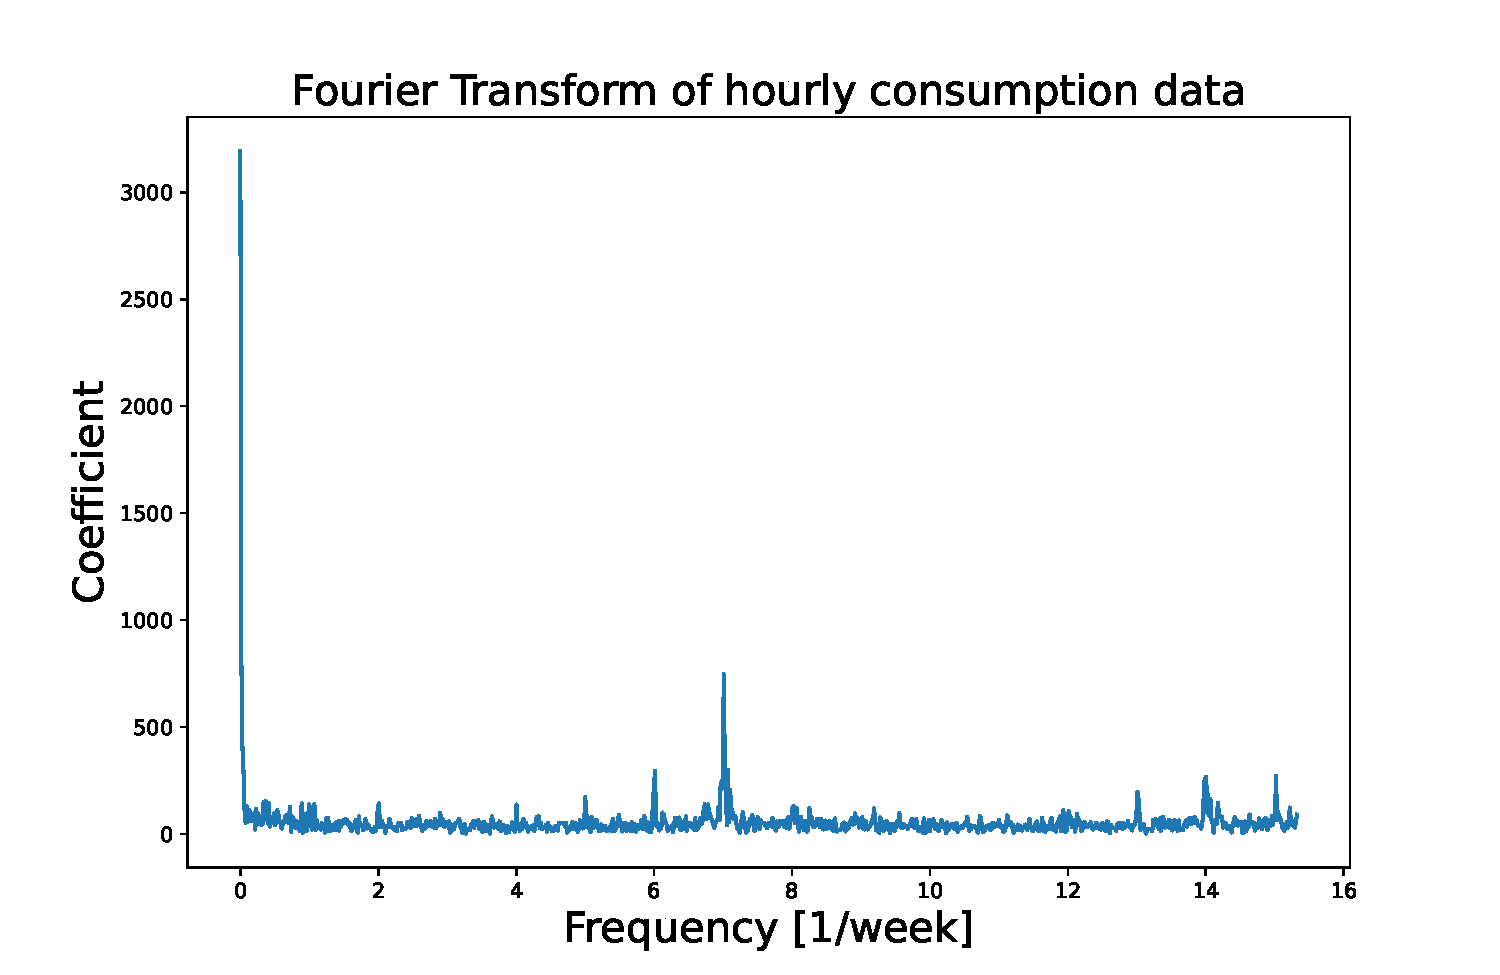
\includegraphics[width=0.8\textwidth]{images/baseline/ft_hour_week_customer1}
\subcaption{First customer.}
\label{fig:ftcustomer1}
\end{minipage}
\ \hspace{2mm} \
\begin{minipage}[b]{8.5cm}
\centering
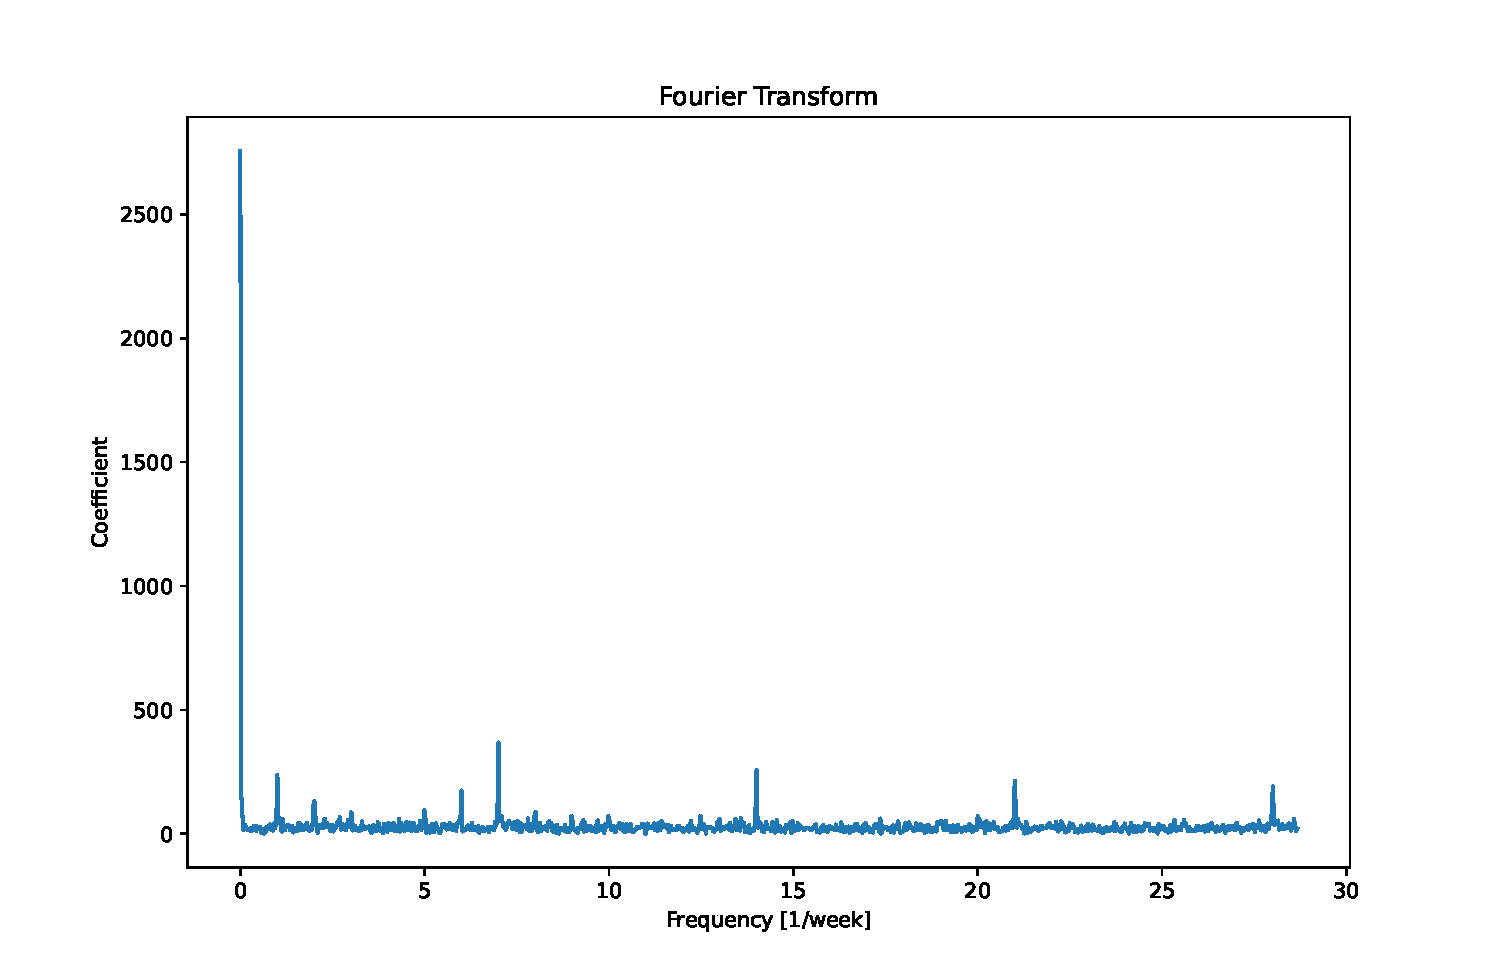
\includegraphics[width=0.8\textwidth]{images/baseline/ft_hour_week_customer2}
\subcaption{Second customer.}
\label{fig:ftcustomer2}
\end{minipage}
\begin{minipage}[b]{17cm}
\centering
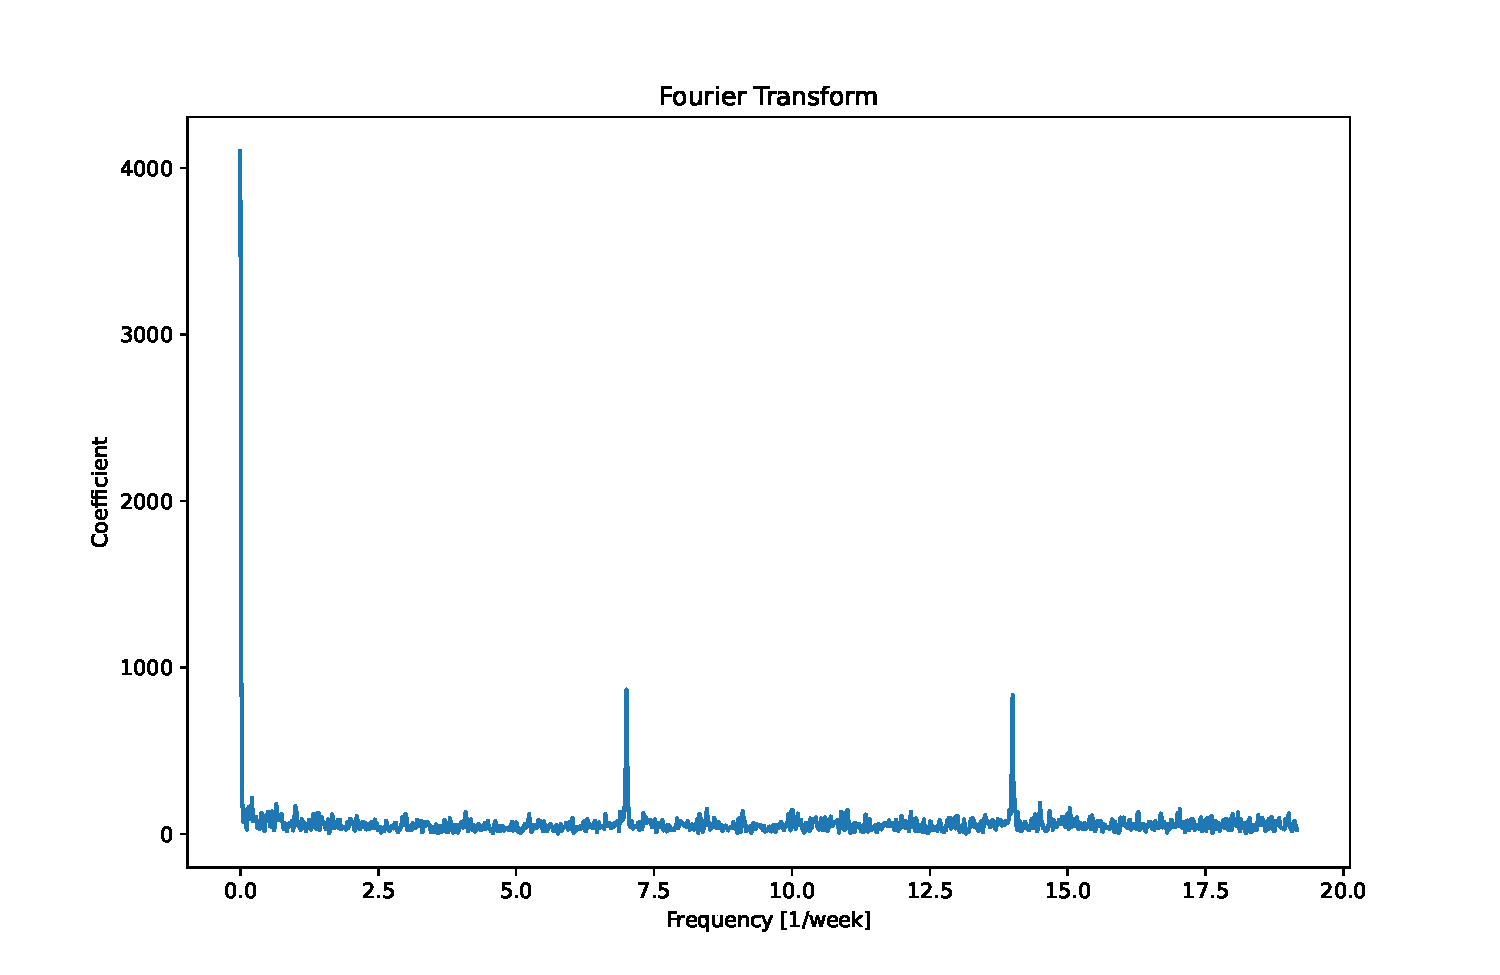
\includegraphics[width=0.4\textwidth]{images/baseline/ft_hour_week_customer3}
\subcaption{Third customer.}
\label{fig:ftcustomer3}
\end{minipage}
\caption{The coefficients given by the Fourier transform of the hourly consumption of the three customers.}
\end{figure}

The daily consumption of the three customers are reported in figure~\ref{fig:dataplotdaycustomer1}, figure~\ref{fig:dataplotdaycustomer2}, and figure~\ref{fig:dataplotdaycustomer3}.

The time series decompositions using an additive model of the daily consumption of the three customers considering as period of the time series a week are reported in figure~\ref{fig:decompositiondaycustomer1}, figure~\ref{fig:decompositiondaycustomer2}, and figure~\ref{fig:decompositiondaycustomer3}.
The decomposition is consistent with the hourly aggregated consumption over the customers.

The auto-correlations of the daily consumption of the three customers are reported in figure~\ref{fig:correlationdaycustomer1},  figure~\ref{fig:correlationdaycustomer2}, and  figure~\ref{fig:correlationdaycustomer3}.
With the daily aggregation, all the customers’ consumptions show are slightly high value with respect to the hourly granularity.
It can be shown that for the first and third customers, the auto-correlation value is slightly high in the closest time lag and then decreases with the days, with a slightly greater value at one week distance.
Instead, for the second customer the only relevant values are only at a multiple of 7 days.

The coefficients given by the Fourier transform for the daily consumption of the three customers are reported in figure~\ref{fig:ftdaycustomer1}, figure~\ref{fig:ftdaycustomer2}, and figure~\ref{fig:ftdaycustomer3}.
The graphical representation exhibits that there are no main frequencies in the daily consumption of the first and third customers.
Instead, for the second customer there is a small peak at the daily periodicity.

\begin{figure}[H]
\begin{minipage}[b]{8.5cm}
\centering
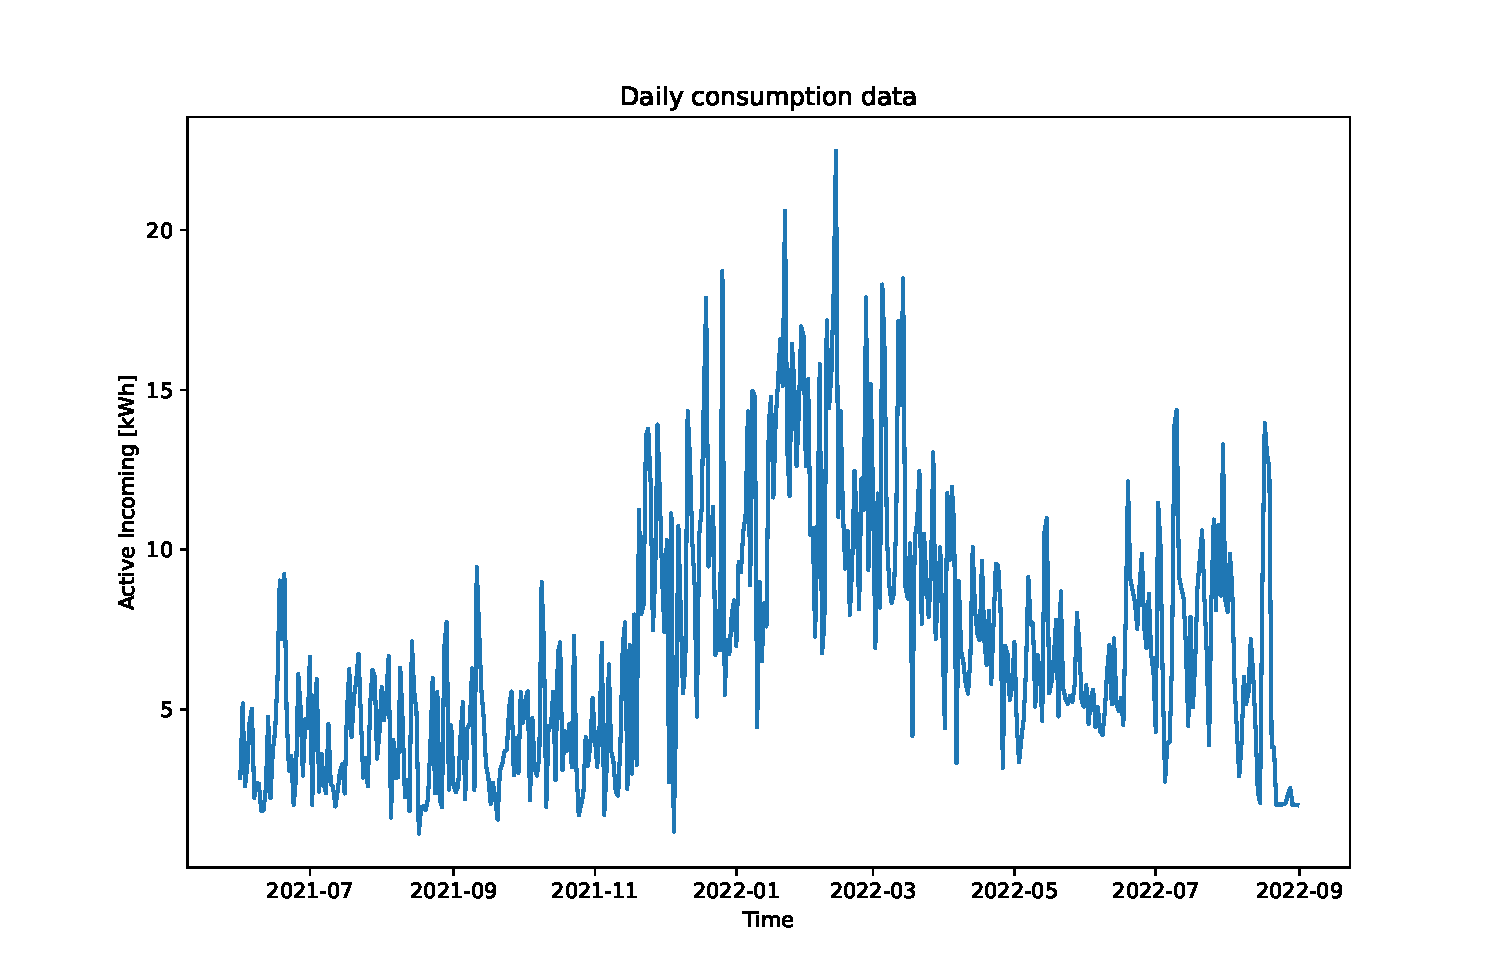
\includegraphics[width=1\textwidth]{images/baseline/data_day_aggregated_plot_customer1}
\subcaption{First customer.}
\label{fig:dataplotdaycustomer1}
\end{minipage}
\ \hspace{2mm} \
\begin{minipage}[b]{8.5cm}
\centering
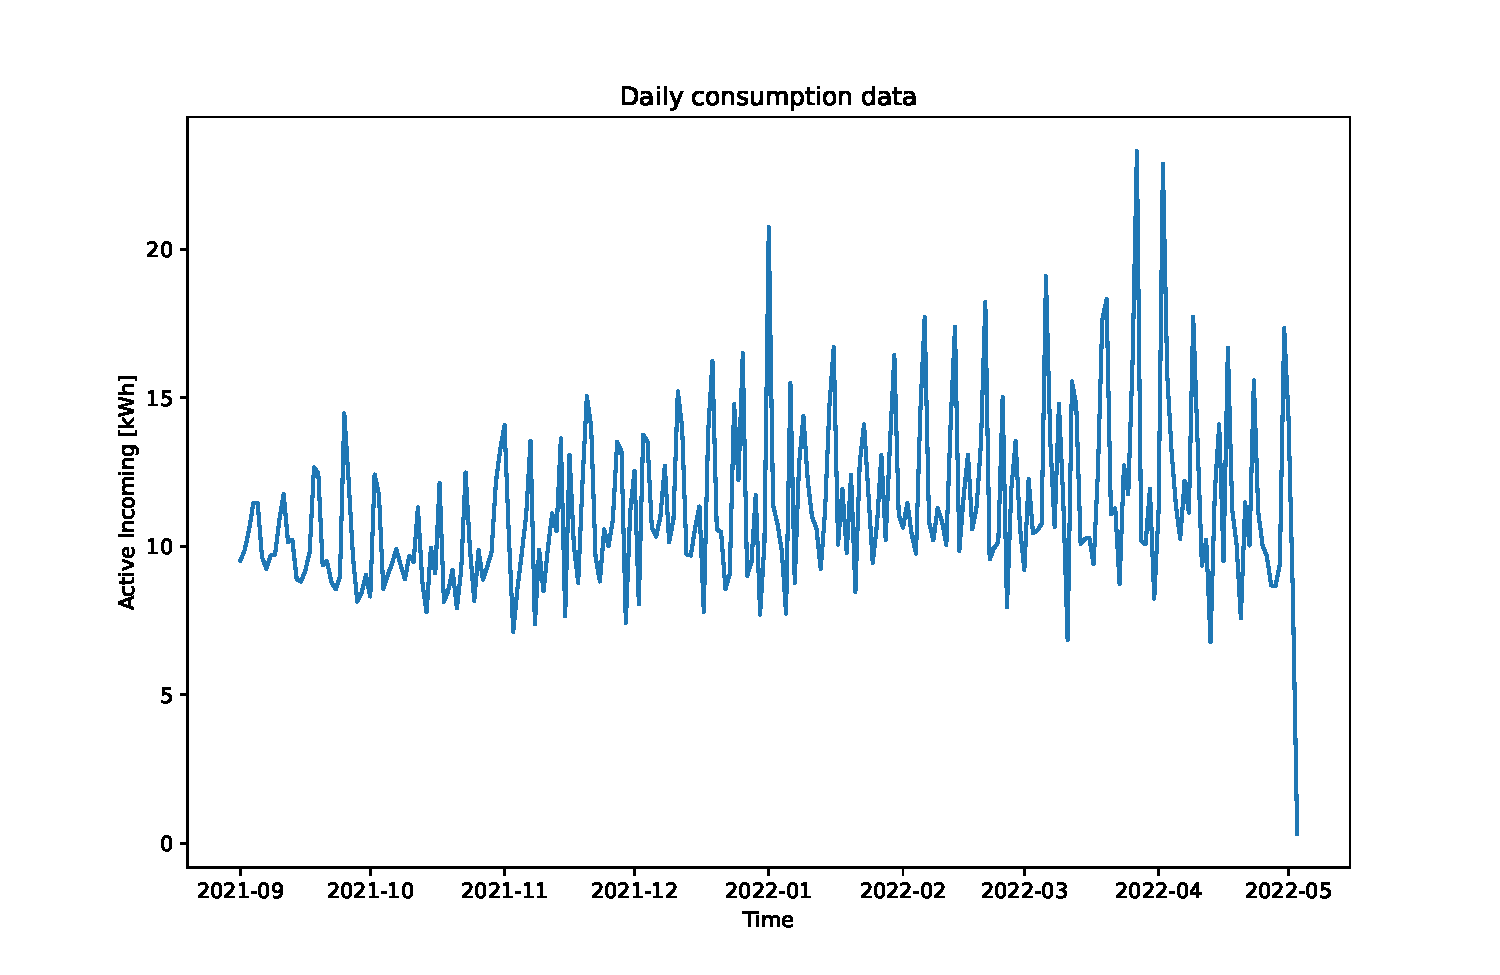
\includegraphics[width=1\textwidth]{images/baseline/data_day_aggregated_plot_customer2}
\subcaption{Second customer.}
\label{fig:dataplotdaycustomer2}
\end{minipage}
\begin{minipage}[b]{17cm}
\centering
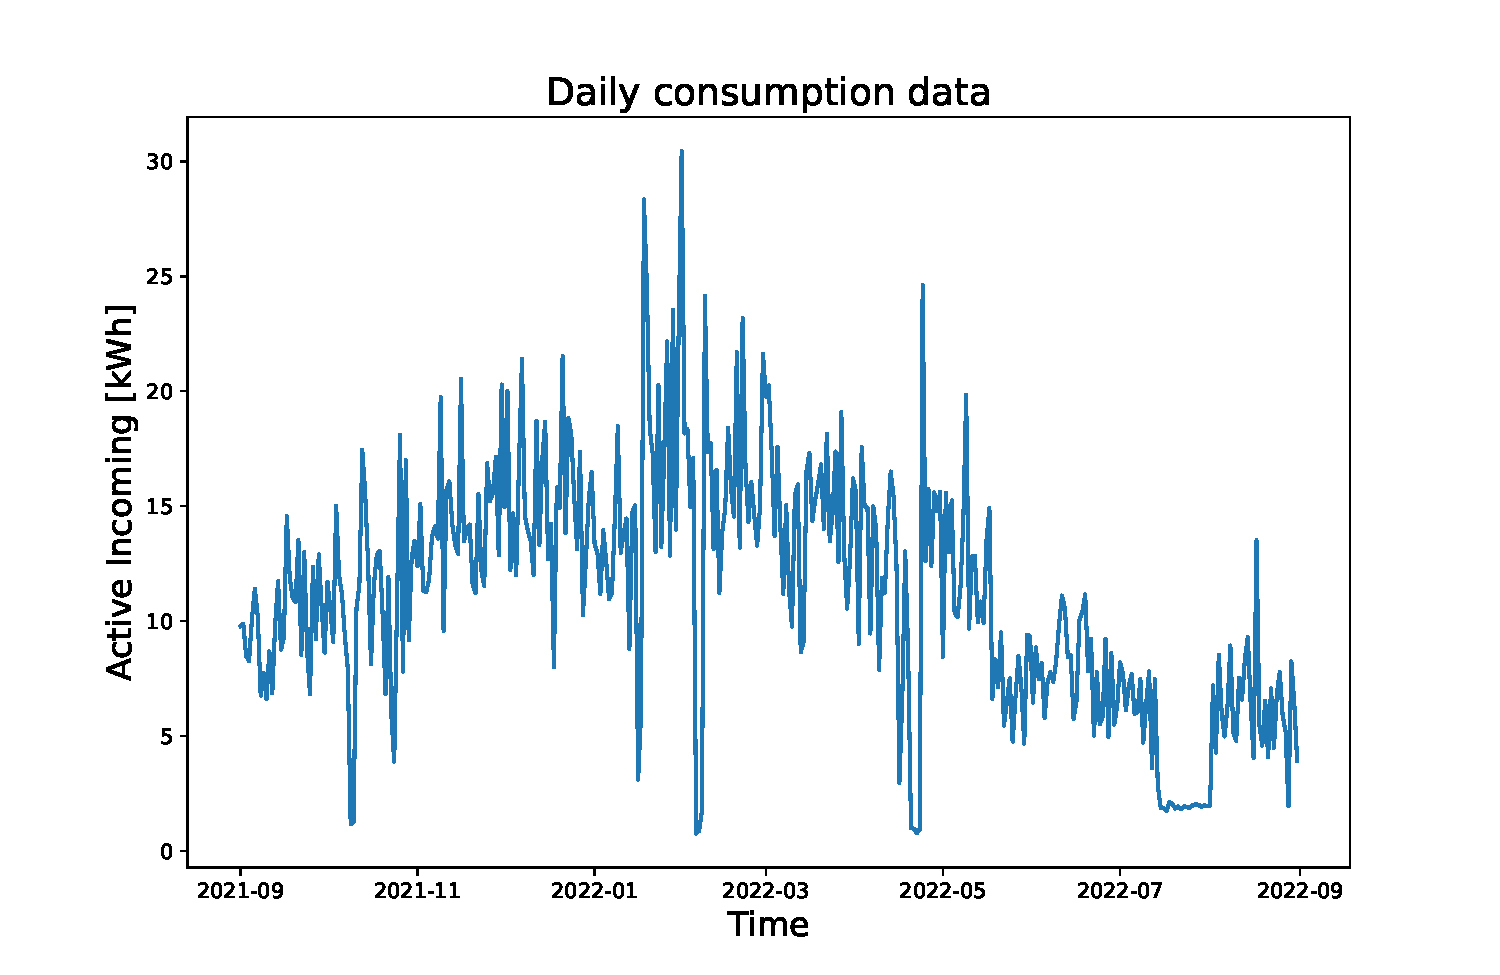
\includegraphics[width=0.5\textwidth]{images/baseline/data_day_aggregated_plot_customer3}
\subcaption{Third customer.}
\label{fig:dataplotdaycustomer3}
\end{minipage}
\caption{The daily consumption of the three customers.}
\end{figure}

As can be noticed from the data, there is high variability in consumption and low auto-correlation, this suggests how it is difficult to produce highly accurate results on a single customer level.
With just the time series of a few users, it is very difficult to learn a well-performing model, having more users it could be possible to learn certain generic trends or standard behaviors.

Basic data is enhanced with the air temperature, the apparent temperature, and the relative humidity since they are considered the only weather features capable of influencing customers' energy consumption.
To assess the relationship between these weather variables and the consumption of the three customers, two correlation coefficients were used: Pearson's correlation coefficient and Spearman's rank correlation coefficient.
Pearson's correlation coefficient measures the strength of the linear relationship between two variables, while Spearman's rank correlation coefficient measures the strength of the monotonic relationship.
The pearsonr and spearmanr methods of the SciPy library were used to compute the correlation with weather data.
The results showed that the hourly consumption of the three customers had:
\begin{itemize}
  \item a Pearson correlation coefficient of -0.2491, 0.0263, and -0.1469 respectively and a Spearman's rank correlation coefficient of -0.2088, 0.1257, and -0.0356 respectively with respect to the air temperature;
  \item a Pearson correlation coefficient of -0.2434, 0.0307, and -0.1494 respectively and a Spearman's rank correlation coefficient of -0.2082, 0.1263, and -0.0366 respectively with respect to the apparent temperature;
  \item a Pearson correlation coefficient of 0.1193, -0.0810, and -0.0753 respectively and a Spearman's rank correlation coefficient of 0.1491, -0.0916, and -0.0814 respectively with respect to the relative humidity.
\end{itemize}
It can be noticed that both the coefficients indicate a weak correlation between the weather variables and the consumption of the three customers, nevertheless, it may still be useful to incorporate weather data into the prediction models since also the auto-correlation values are not particularly high.

\begin{figure}[H]
\begin{minipage}[b]{8.5cm}
\centering
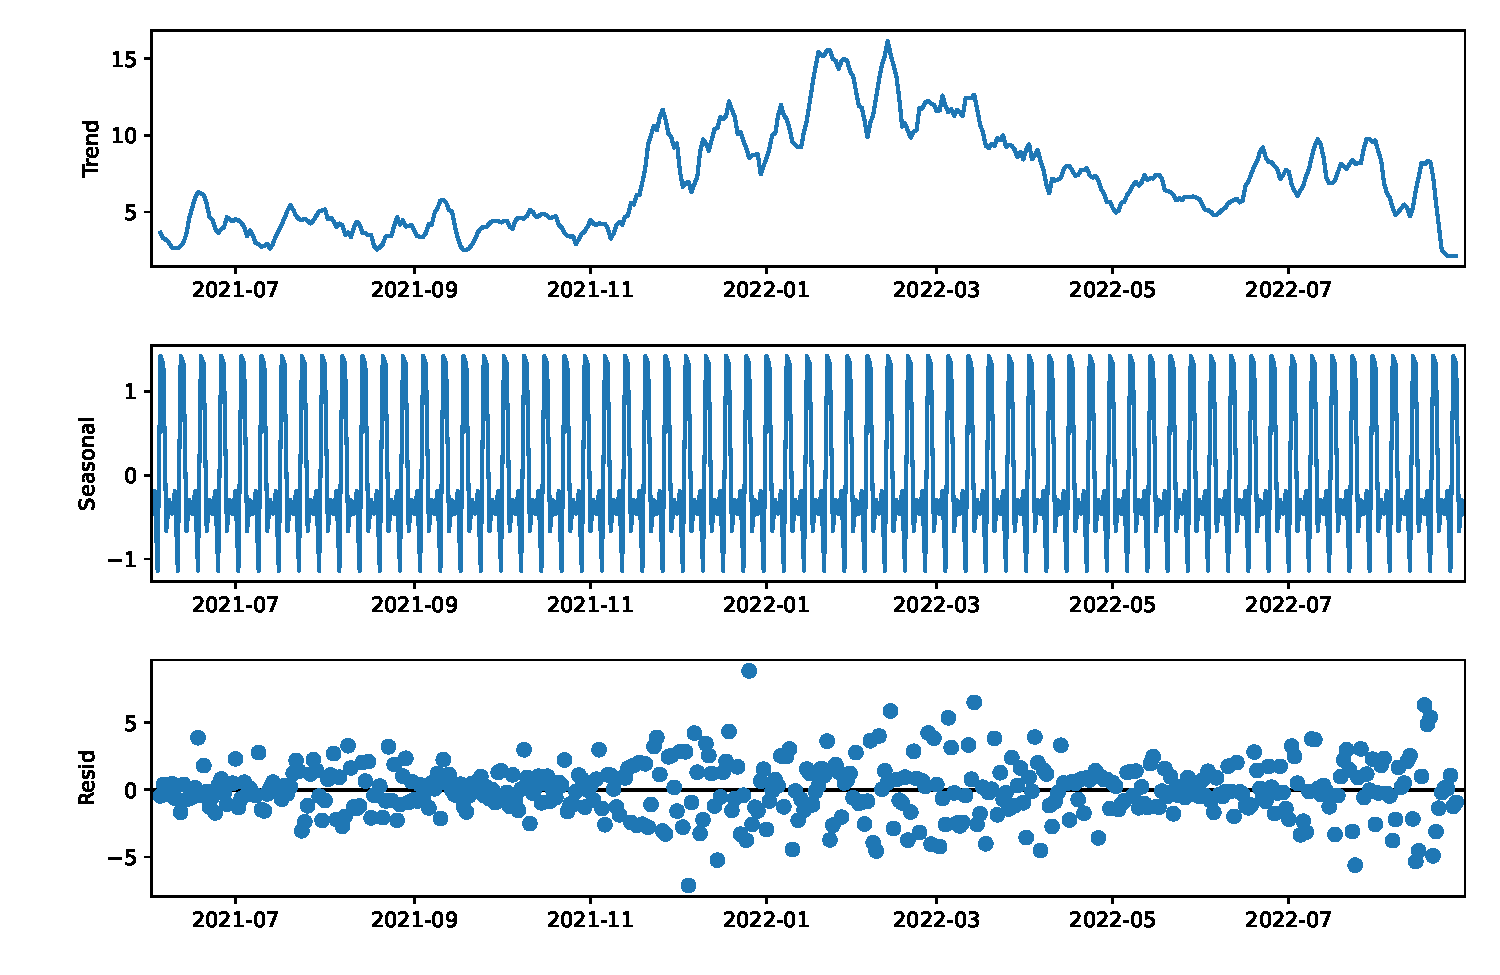
\includegraphics[width=1\textwidth]{images/baseline/daily_aggregated_decomposition_customer1}
\subcaption{First customer.}
\label{fig:decompositiondaycustomer1}
\end{minipage}
\ \hspace{2mm} \
\begin{minipage}[b]{8.5cm}
\centering
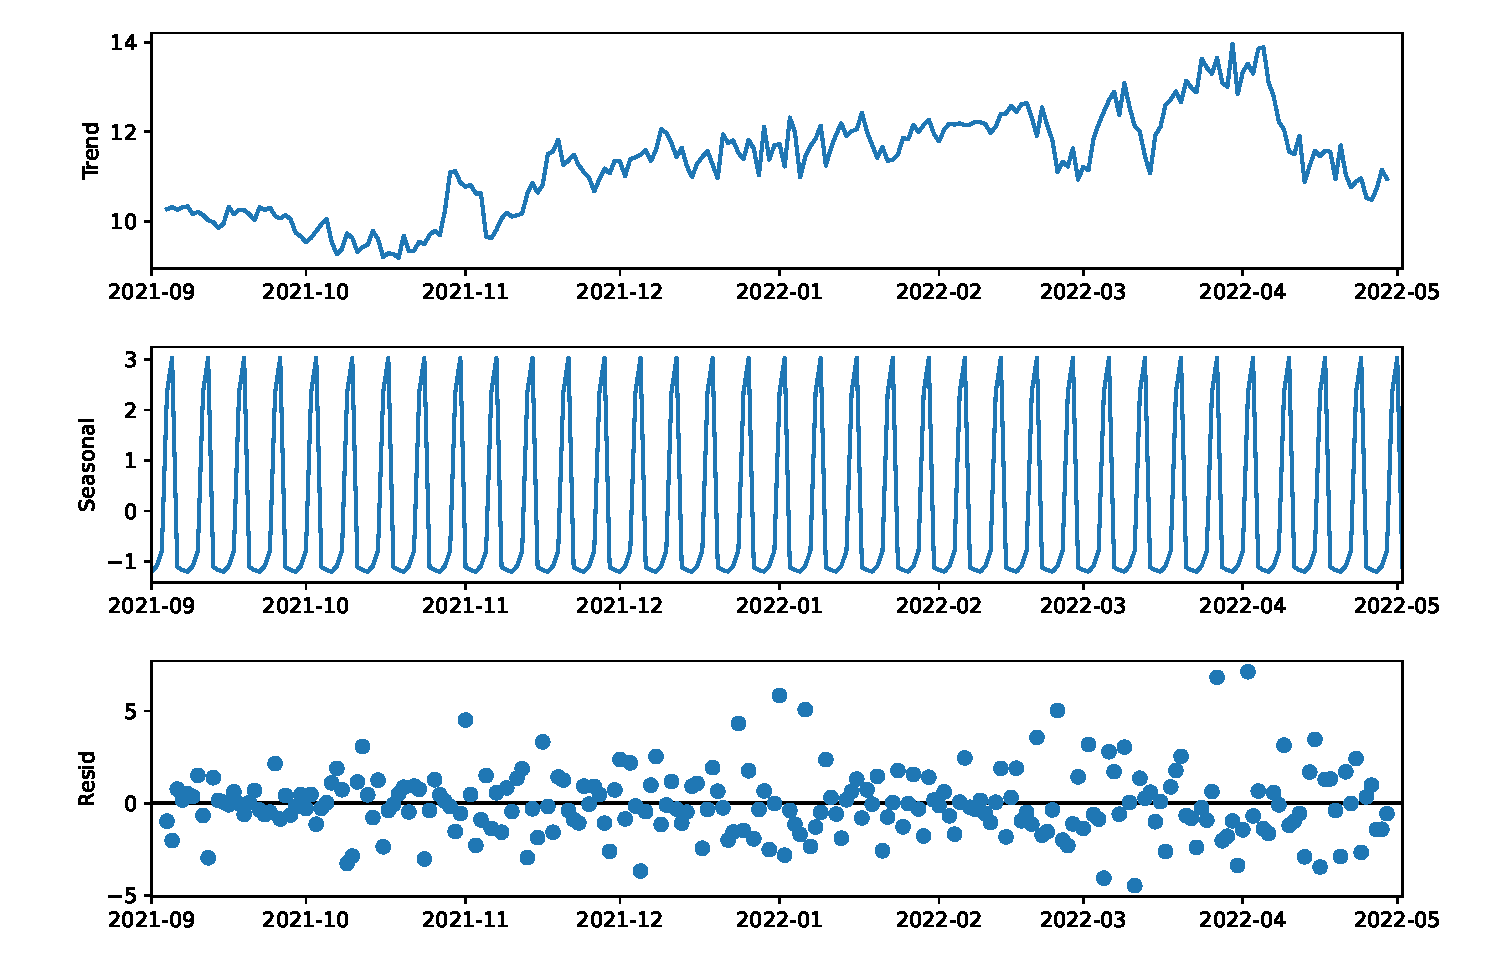
\includegraphics[width=1\textwidth]{images/baseline/daily_aggregated_decomposition_customer2}
\subcaption{Second customer.}
\label{fig:decompositiondaycustomer2}
\end{minipage}
\begin{minipage}[b]{17cm}
\centering
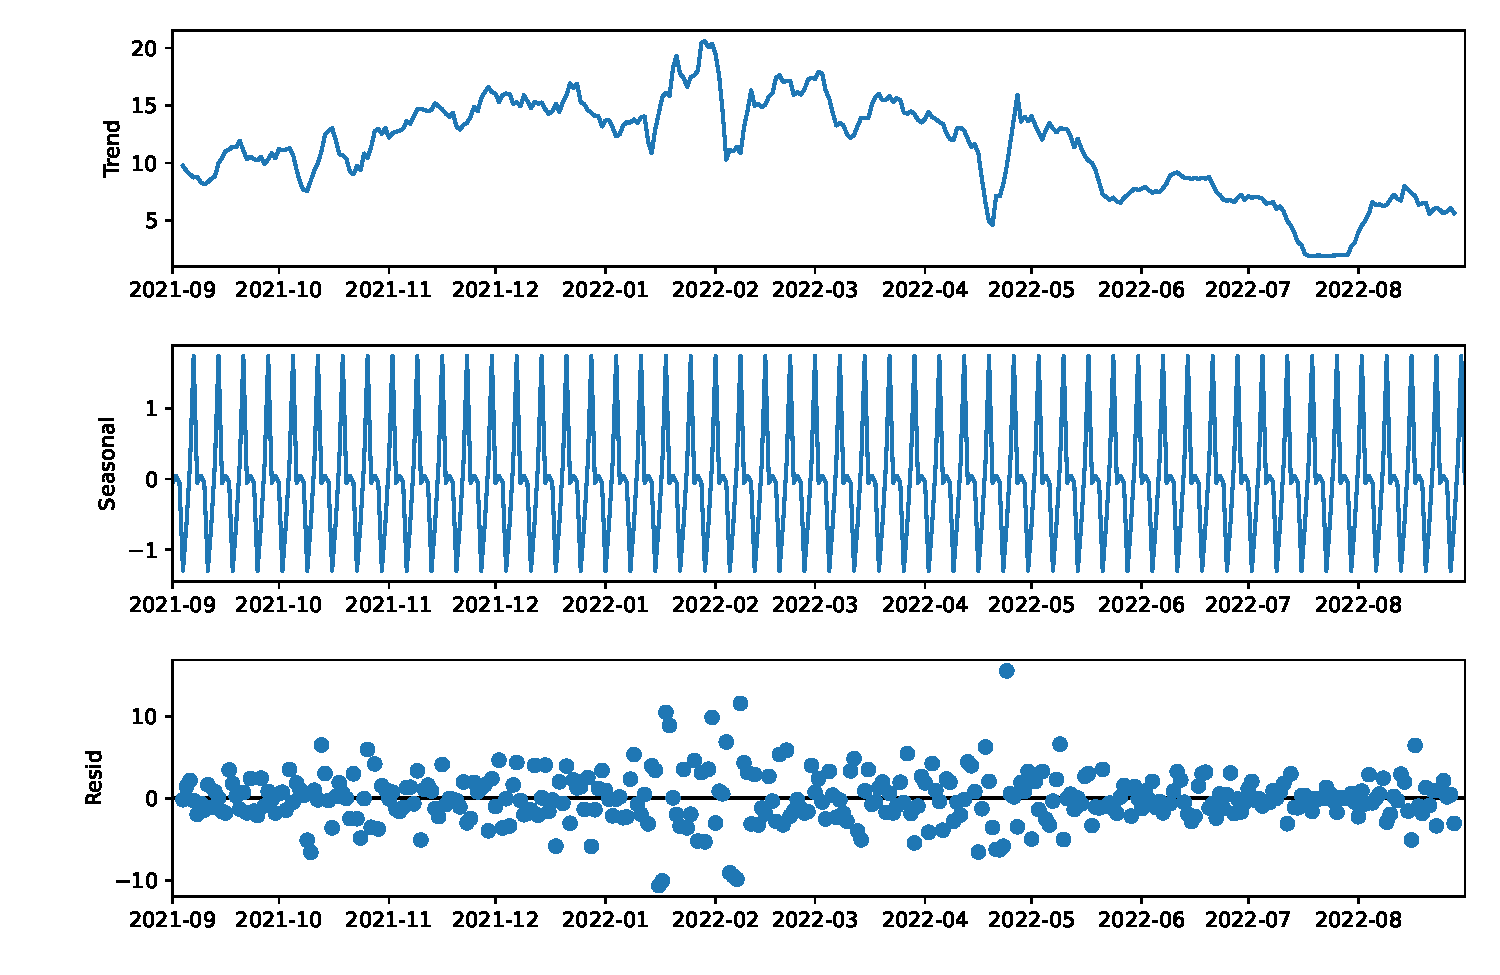
\includegraphics[width=0.5\textwidth]{images/baseline/daily_aggregated_decomposition_customer3}
\subcaption{Third customer.}
\label{fig:decompositiondaycustomer3}
\end{minipage}
\label{fig:decompositiondaycustomer}
\caption{The time series decompositions of the daily consumption of the three customers considering as period of the time series a week.}
\end{figure}

\begin{figure}[H]
\begin{minipage}[b]{8.5cm}
\centering
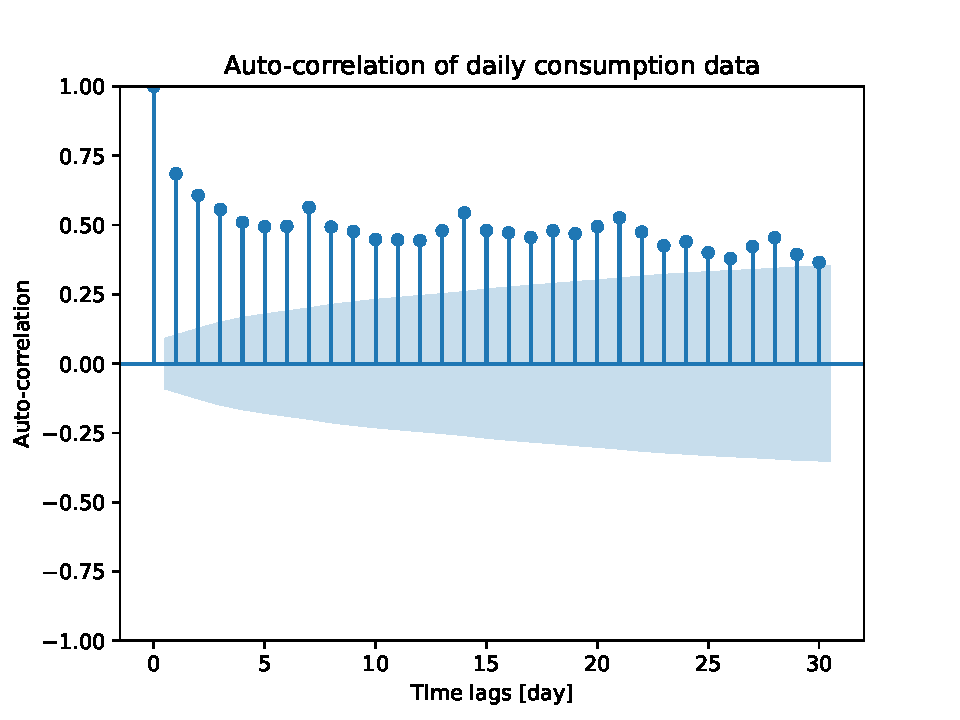
\includegraphics[width=0.8\textwidth]{images/baseline/daily_aggregated_correlation_customer1}
\subcaption{First customer.}
\label{fig:correlationdaycustomer1}
\end{minipage}
\ \hspace{2mm} \
\begin{minipage}[b]{8.5cm}
\centering
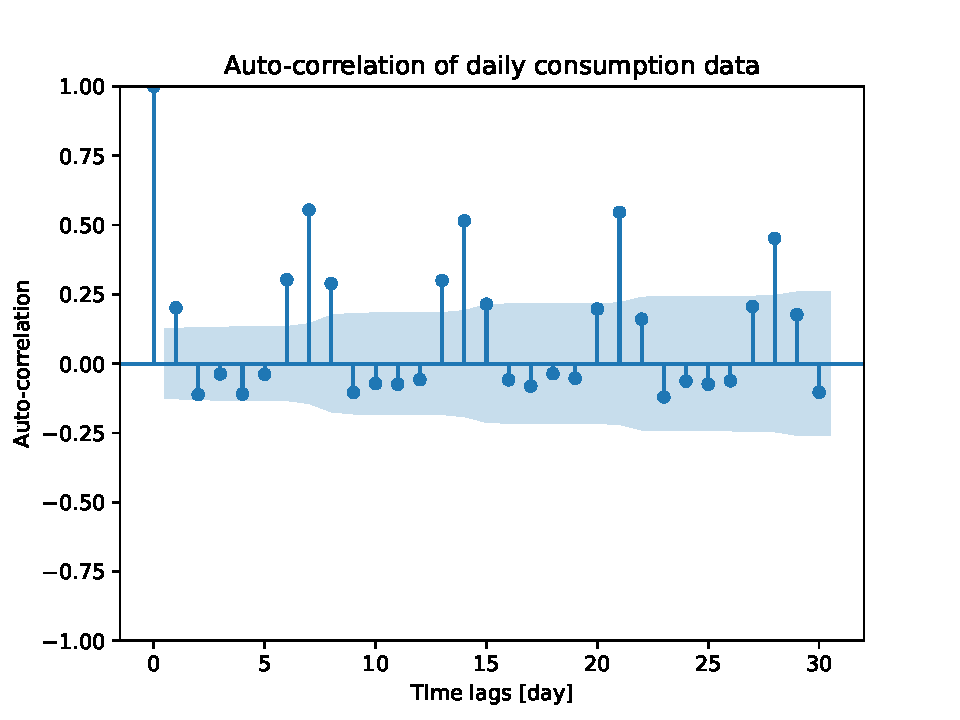
\includegraphics[width=0.8\textwidth]{images/baseline/daily_aggregated_correlation_customer2}
\subcaption{Second customer.}
\label{fig:correlationdaycustomer2}
\end{minipage}
\begin{minipage}[b]{17cm}
\centering
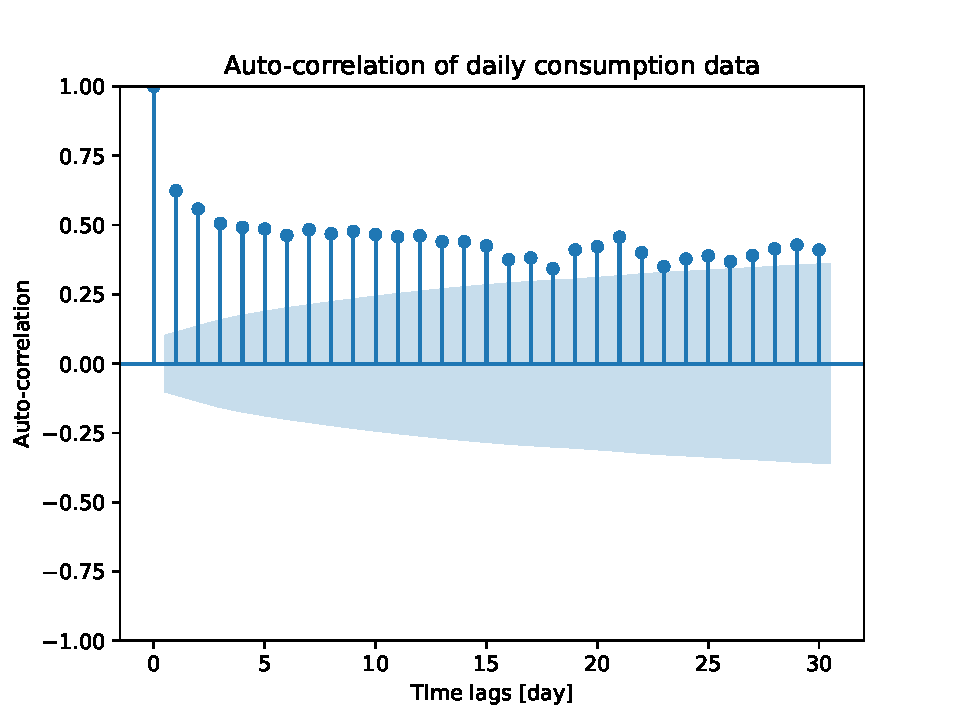
\includegraphics[width=0.4\textwidth]{images/baseline/daily_aggregated_correlation_customer3}
\subcaption{Third customer.}
\label{fig:correlationdaycustomer3}
\end{minipage}
\caption{The auto-correlations of the daily consumption of the three customers.}
\end{figure}

\begin{figure}[H]
\begin{minipage}[b]{8.5cm}
\centering
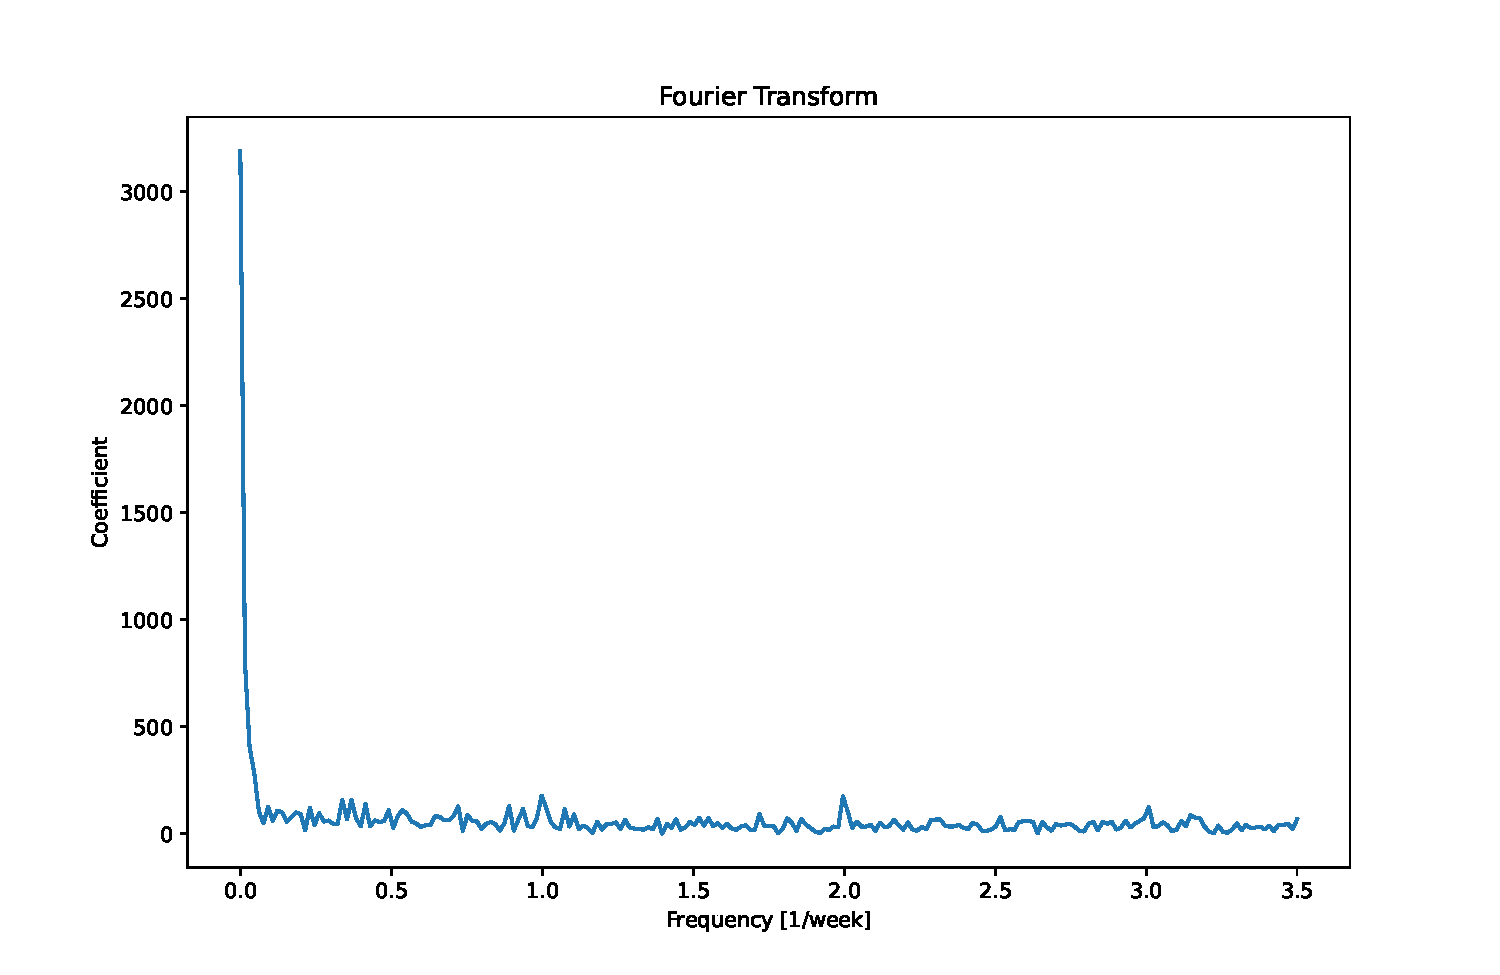
\includegraphics[width=0.8\textwidth]{images/baseline/ft_day_customer1}
\subcaption{First customer.}
\label{fig:ftdaycustomer1}
\end{minipage}
\ \hspace{2mm} \
\begin{minipage}[b]{8.5cm}
\centering
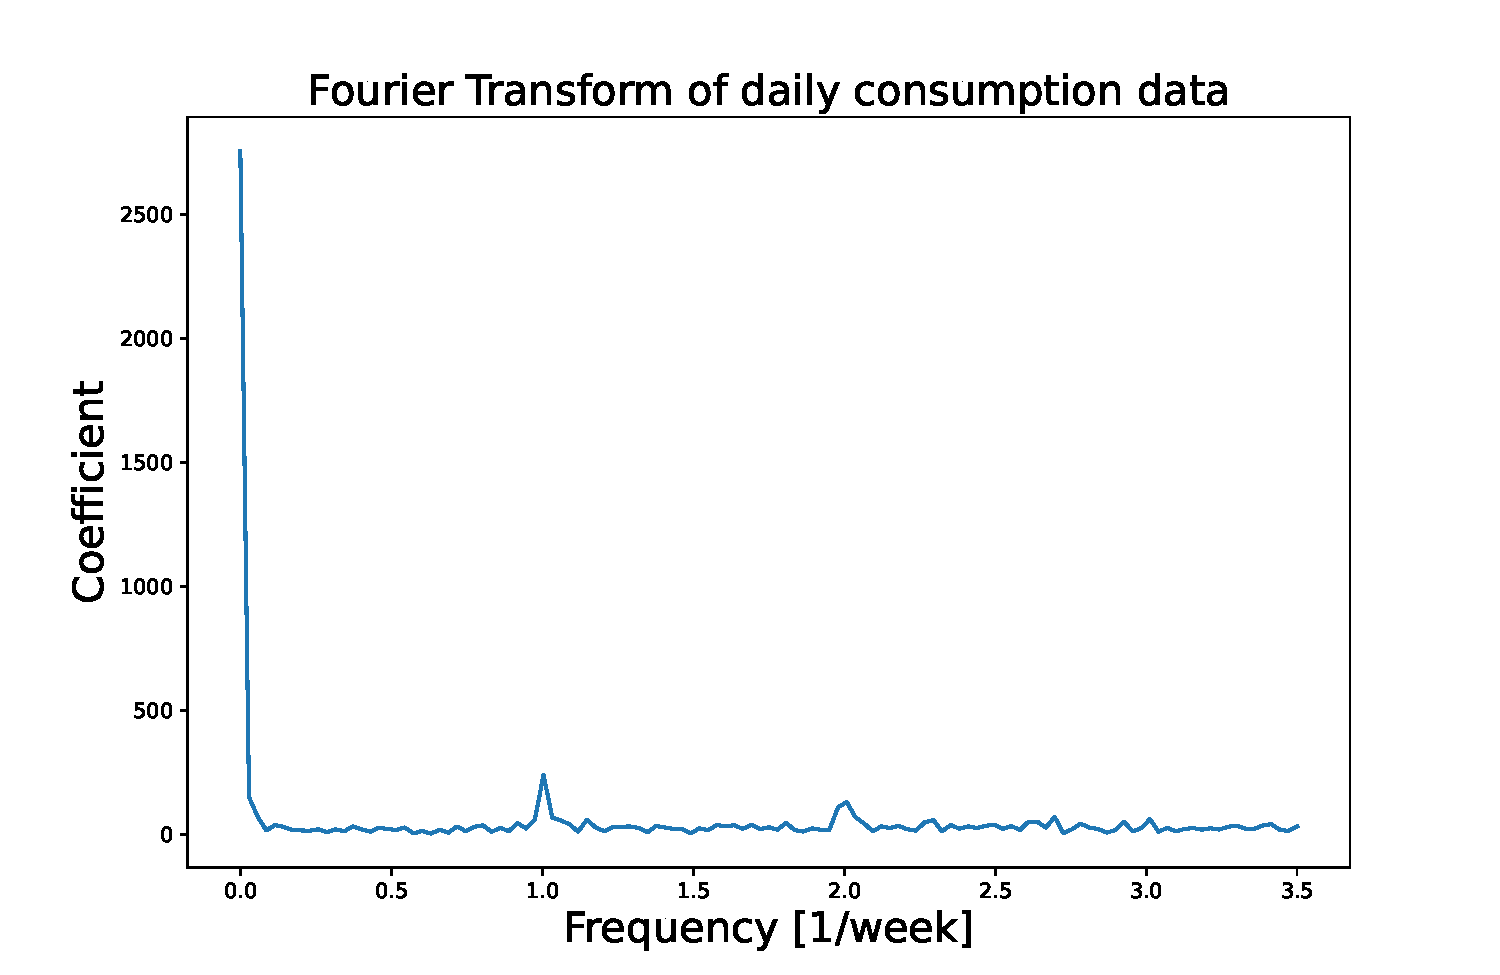
\includegraphics[width=0.8\textwidth]{images/baseline/ft_day_customer2}
\subcaption{Second customer.}
\label{fig:ftdaycustomer2}
\end{minipage}
\begin{minipage}[b]{17cm}
\centering
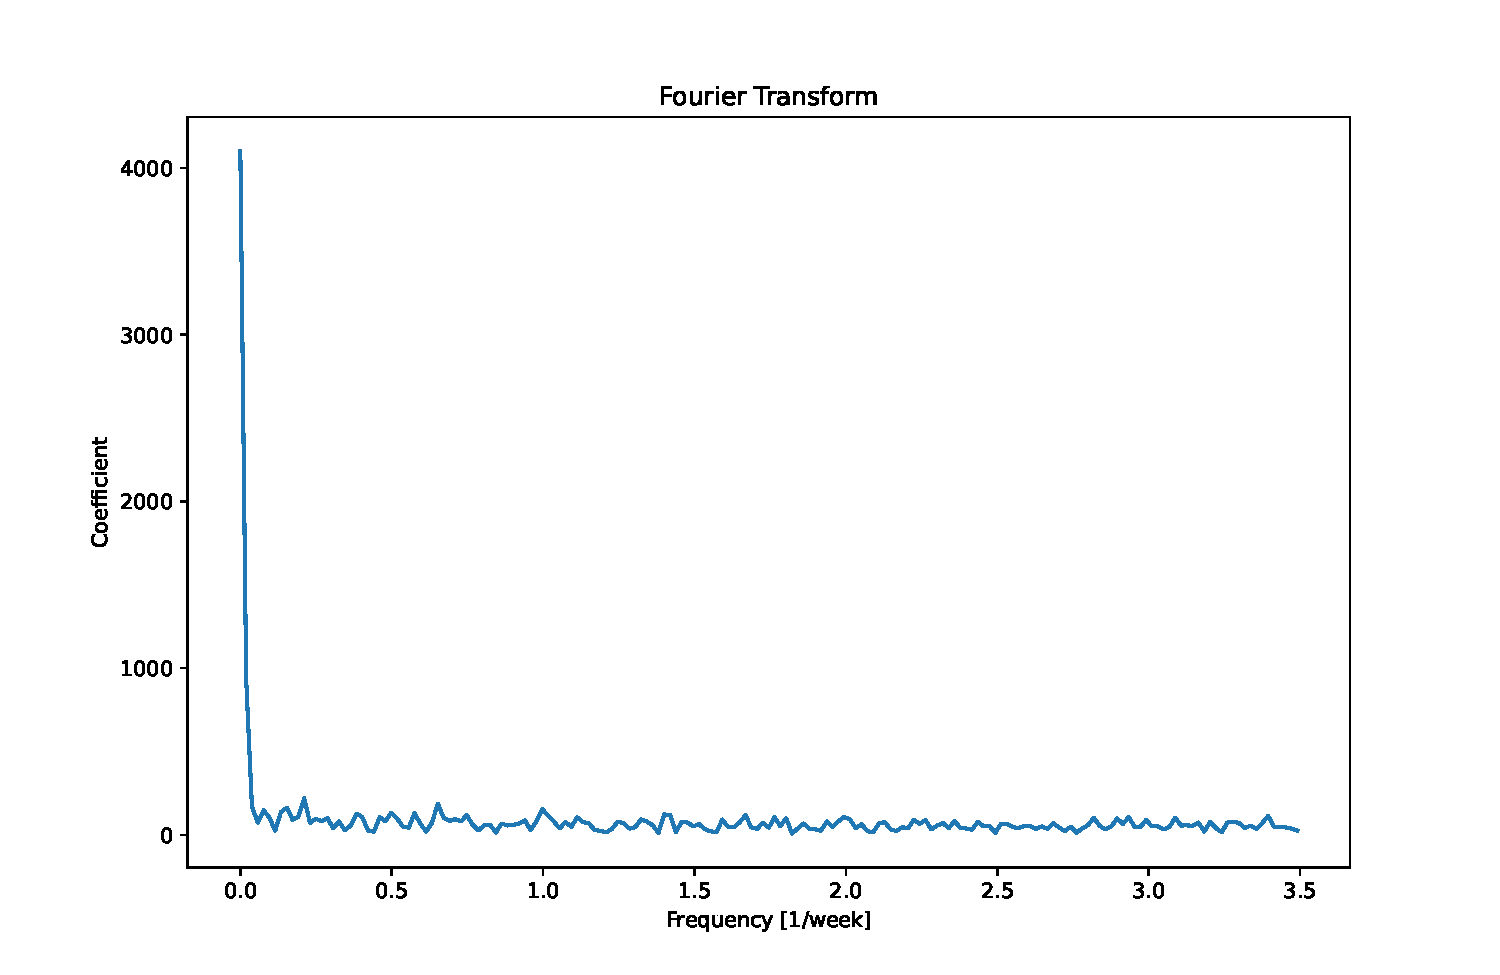
\includegraphics[width=0.4\textwidth]{images/baseline/ft_day_customer3}
\subcaption{Third customer.}
\label{fig:ftdaycustomer3}
\end{minipage}
\caption{The coefficients given by the Fourier transform of the daily consumption of the three customers.}
\end{figure}

The results showed that the daily consumption of the three customers had:
\begin{itemize}
  \item a Pearson correlation coefficient of -0.5538, -0.2286, and -0.6707 respectively and a Spearman's rank correlation coefficient of -0.5154, -0.2639, and -0.6949 respectively with respect to the air temperature;
  \item a Pearson correlation coefficient of -0.5356, -0.2276, and -0.6768 respectively and a Spearman's rank correlation coefficient of -0.5156, -0.2634, and -0.6975 respectively with respect to the apparent temperature;
  \item a Pearson correlation coefficient of 0.1241, 0.0100, and 0.1368 respectively and a Spearman's rank correlation coefficient of 0.1381, 0.0409, and 0.2077 respectively with respect to the relative humidity.
\end{itemize}
It can be noticed that both the coefficients increased considering the daily data meaning that the mean weather data over the day is more correlated to the daily consumption of the three considered customers, compared to the hourly granularity.

% TODO What about tariff aggregation, probably not to include?

Describe the choice of parameters for models ... (list with motivations)

Analyze the forecasts of the models for the electricity demand forecasting task (predictive analytics) ...
% TODO ancora da ultimare SARIMA o arima su serie equipollente e AutoML su altre granularità
12 splits were used for block validation with a test size of 168 each time. % TODO

Summary table with results ...
% TODO where results are the one given by cross-validation mean ± std
% TODO check the consistency of model results in the last period and using cross-validation --> do a table with the differences (+ plot for internal analysis)
% commentarli (sia il numero che il grafico dell’errore) --> interpretare il dato (perchè è buono?) --> benchmark in letteratura, ecc…
% [valutare criticamente, aspetto tecnologico scientifico]
